% =============================================================================
% draft.tex
% =============================================================================
% Compilation (keeps the directory clean):
%   latexmk -xelatex -interaction=nonstopmode -halt-on-error -file-line-error -synctex=0 draft.tex
%   latexmk -c draft.tex
%
% Manual compilation (then delete intermediates):
%   xelatex  draft
%   biber    draft
%   xelatex  draft
%   xelatex  draft
% =============================================================================

\documentclass[11pt]{article}

\usepackage[margin=1in]{geometry}
\usepackage{amsmath,amssymb,amsthm}
\usepackage{setspace}
\usepackage{enumitem}
\usepackage{array}
\usepackage{booktabs}
\usepackage{graphicx}
\usepackage{float}
\usepackage{tikz}
\usepackage[hidelinks]{hyperref}
\usepackage[backend=biber,style=authoryear,natbib=true,maxcitenames=2,maxbibnames=99]{biblatex}
\addbibresource{bibliography.bib}

\setstretch{1.1}

% Theorem environments
\newtheorem{theorem}{Theorem}
\newtheorem{proposition}{Proposition}
\newtheorem{lemma}{Lemma}
\newtheorem{corollary}{Corollary}
\newtheorem{definition}{Definition}

% Commands
\newcommand{\E}{\mathbb{E}}
\newcommand{\PP}{\mathbb{P}}
\newcommand{\1}{\mathbf{1}}
\newcommand{\Var}{\mathrm{Var}}
\newcommand{\Cov}{\mathrm{Cov}}
\newcommand{\R}{\mathbb{R}}
% ---- macros + theorem envs required by the Equilibrium-foundations splice (D6) and Dominance Lemma (S2) ----
\newtheorem{assumption}{Assumption}
\newtheorem{remark}{Remark}
\providecommand{\kp}{\kappa}
\providecommand{\kvec}{\mathbf{k}}
\providecommand{\kone}{k_1}
\providecommand{\kzero}{k_0}
\providecommand{\kD}{k_D}
\providecommand{\Tmap}{T}
\providecommand{\Psifp}{\Psi}
\providecommand{\Dmin}{\Delta^{\min}}
\providecommand{\mt}{\tilde{m}}
\providecommand{\vhat}{\hat{v}}
\providecommand{\Vhat}{\hat{V}}
\providecommand{\Sbar}{\bar{S}}
\providecommand{\Kcost}{K}
\providecommand{\sigxi}{\sigma_\xi}
\providecommand{\sv}{\sigma_v}
\providecommand{\deltaliq}{\delta}
\providecommand{\Ccost}{C}
\providecommand{\chivar}{\chi}
\providecommand{\pibar}{\bar{\pi}}
\providecommand{\omegaH}{\omega_H}
\providecommand{\omegaQ}{\omega_Q}
\providecommand{\omegaP}{\omega_P}
\providecommand{\xibid}{\xi}

\title{\textbf{Liquidity, Activism Disclosure, and Takeover Premia:}\\[0.3em]
\large A Theory of Exit, Voice, and Corporate Control}
\author{Austin Li\\[0.25em]}
\date{}

\begin{document}
\maketitle


%==============================================================================
\begin{abstract}
\noindent How does a stake-triggered disclosure threshold shape the liquidity sensitivity of takeover premia? I develop a takeover model in which an informed blockholder, observing a private signal about firm value, chooses among Exit (sell the stake), Hold (retain passively), Quiet Voice (engage below the disclosure threshold), and Public Voice (accumulate shares, engage, and trigger mandatory disclosure). A market maker prices from order flow and the disclosure flag, and a potential bidder conditions entry on these market signals. Disclosure partitions order-flow inference into a disclosed branch, where the activism premium is directly observed, and a nondisclosed branch, where it is merely inferred. The central result is a disclosure-attenuation theorem: by moving the activism premium from an inferred to a directly observable basis, stricter disclosure makes takeover premia less sensitive to market liquidity, predicting lower liquidity sensitivity in strict-disclosure jurisdictions. As a supporting comparative static, under a transparent primitive condition on the price-elasticity of bids, the premium captured by minority shareholders is single-peaked in liquidity, with exact endpoint symmetry $\Delta^{\min}(0)=\Delta^{\min}(1)$, so an interior, premium-maximizing liquidity level $\kappa^{\dagger}$ exists and its location is governed by the disclosure threshold. Rising noise-trading intensity lowers adverse-selection costs but erodes the informativeness of order flow, pushing bid incidence and engagement incentives in opposing directions; the interior optimum reflects this balance and is driven by the disclosure regime rather than by the activism technology.
\end{abstract}

\newpage

%==============================================================================
\section{Introduction}
%==============================================================================

When an activist investor discovers underperformance at a portfolio company, she faces a consequential choice: sell her stake and move on, engage quietly behind the scenes, or accumulate shares aggressively enough to cross a regulatory disclosure threshold. Each path carries different risks and rewards, and each sends different signals to the market. How she resolves this dilemma shapes not only her own returns but whether a takeover bid emerges and what minority shareholders ultimately receive. This tension is the classic exit-versus-voice problem of \citet{Hirschman1970}, transplanted into financial markets. On one side, liquidity facilitates governance by letting activists accumulate stakes cheaply and reducing free-riding \citep{Maug1998}. On the other, liquidity makes selling painless, tempting blockholders to exit rather than bear the costs of engagement \citep{Coffee1991,Bhide1993}. The tension deepens once we recognize that prices are not passive scorekeepers: when takeover decisions depend on stock prices, trading has real effects through feedback channels \citep{BondEdmansGoldstein2012,EdmansGoldsteinJiang2012}. Consequently, the blockholder's choice between exit and voice reverberates beyond her portfolio into the real economy. Existing models isolate these forces rather than combining them; this paper is the first to let stake-triggered disclosure partition order-flow inference into disclosed and nondisclosed branches and feed that inference into endogenous bidder entry, yielding a single equilibrium object in which endogenous governance choice, order-flow inference, and takeover feedback are jointly determined.

To fill this gap, I develop a model in which a blockholder observes a private signal about firm value and chooses among four actions: Exit (sell her stake), Hold (retain without engaging), Quiet Voice (engage below the disclosure threshold), or Public Voice (buy additional shares, engage, and trigger mandatory disclosure). A competitive market maker sets prices from discrete order flow and the disclosure flag, while a potential bidder conditions entry on these market signals. Engagement raises standalone value and strengthens resistance to acquisition, increasing the premium a bidder must offer. The key modeling choice is that disclosure is stake-triggered: activism is directly observable only when the blockholder crosses a regulatory threshold, creating two distinct information regimes within a single equilibrium.

The model yields two main results. First, liquidity has a nonmonotone effect on expected minority takeover gains. At low liquidity, noise trading is scarce, making the blockholder's orders highly informative. The market maker largely infers her action, which deters quiet engagement and suppresses bids. As liquidity rises, noise camouflages the activist's trades, encouraging voice and improving bid incidence. However, at high liquidity, exit becomes so cheap that engagement incentives collapse entirely. The net effect is hump-shaped: minority shareholders benefit most at intermediate liquidity, where voice is both incentive-compatible and partially concealed. Second, stake-triggered disclosure attenuates this inference channel. Lowering the disclosure threshold shifts probability mass from Quiet Voice to Public Voice, compressing the activism premium into the observable regime and making it less sensitive to liquidity. The model predicts that the sensitivity of takeover premia to liquidity is lower in strict-disclosure jurisdictions.

These theoretical mechanisms speak directly to active policy debates. The United States Schedule 13D threshold of 5\% and the United Kingdom FCA threshold of 3\% create meaningfully different information environments. The framework provides a rigorous way to evaluate how such cross-country differences affect takeover outcomes and minority shareholder welfare, revealing that liquidity regulation operates implicitly as governance policy.

The model's predictions are motivated by well-documented empirical patterns. \citet{BravJiangPartnoyThomas2008} show that hedge fund activism often targets firms that subsequently receive acquisition offers. \citet{GreenwoodSchor2009} find that a substantial fraction of activist returns is attributable to takeover outcomes. The free-rider problem that \citet{GrossmanHart1980} identified in tender offers makes takeover premia the natural welfare object for dispersed minority shareholders, underscoring the importance of understanding how liquidity shapes these outcomes.

The paper proceeds as follows. Section~\ref{sec:lit} reviews the literature. Section~\ref{sec:model} presents the model, and Section~\ref{sec:equilibrium} characterizes the equilibrium. Section~\ref{sec:numerical} develops comparative statics with numerical analysis. Section~\ref{sec:testable} presents testable implications. Sections~\ref{sec:welfare} and~\ref{sec:extensions} analyze welfare and disclosure extensions. Section~\ref{sec:conclusion} concludes.
\section{Related Literature}
\label{sec:lit}
%==============================================================================

This paper connects three strands of the finance literature (blockholder governance, market microstructure, and corporate takeovers) and shows that their interaction produces equilibrium effects that no single strand generates alone.

Three recent papers are especially close, and the contribution is sharpest when set against them. \citet{OrdonezCalafiBernhardt2022} study the optimal \emph{design} of the beneficial-ownership disclosure threshold, weighing the adverse-selection cost it imposes on uninformed investors against the activism it disciplines; here the threshold is instead taken as an institutional primitive whose equilibrium role is to partition order-flow inference and, through that channel, shape takeover premia. \citet{CorumLevit2019} model activists as catalysts of corporate control via contracting with bidders, but abstract from the secondary-market inference and disclosure regimes that are central here. Finally, \citet{CetemenCisternasKolbViswanathan2026} provide a dynamic account in which multiple activists time their trades sequentially and coordinate through market signals, producing leader-follower dynamics; this paper is its static counterpart, with a single blockholder whose threshold-crossing disclosure splits order-flow inference into disclosed and nondisclosed branches that in turn feed bidder entry.

%
\subsection{Exit vs.\ Voice in Corporate Governance}
%

The exit-voice trade-off originates with \citet{Hirschman1970}. Early applications treated the two as substitutes, arguing that liquidity weakens governance by allowing blockholders to flee rather than fight \citep{Coffee1991,Bhide1993}. \citet{Maug1998} reversed this logic, demonstrating that liquidity can facilitate voice by easing stake accumulation. \citet{Edmans2009} recast exit itself as a governance mechanism, showing that trading on bad private information punishes underperforming managers through equity-linked compensation. \citet{EdmansManso2011} extend this to multiple blockholders, while \citet{EdmansFangZur2013} provide empirical evidence that liquidity shifts blockholders toward exit and away from voice. \citet{LevitMalenkoMaug2024} further show that trading reshapes the shareholder base and interacts with governance through voting, complementing the exit-voice trade-off studied here.\footnote{A common feature of these governance models is continuous trading. The present paper departs from that tradition by adopting discrete order flow, which keeps the inference problem tractable when integrating both disclosure regimes and price feedback.}

%
\subsection{Market Microstructure and Price Feedback}
%

Microstructure models explain how prices aggregate private information through trading \citep{Kyle1985,GlostenMilgrom1985}. I build on the tractable discrete order-flow framework of \citet{EdmansGoldsteinJiang2015}, which permits closed-form Bayesian updating and clear price fixed points. Financial prices also shape real economic decisions through feedback channels. \citet{EdmansGoldsteinJiang2012} demonstrate that stock prices affect takeover outcomes: low prices signal weak fundamentals and invite bids, while high prices deter them. \citet{BondEdmansGoldstein2012} survey this broader feedback literature; \citet{Goldstein2023} provides a more recent synthesis of how market information feeds back into real corporate decisions.\footnote{\citet{DowGoldsteinGuembel2017} provide foundations for endogenous information production in settings where prices affect real investment.} None of these frameworks, however, allow an informed blockholder to choose between exit and voice before prices form.

%
\subsection{Shareholder Activism and Takeovers}
%

Empirical evidence firmly links activism to corporate control. \citet{BravJiangPartnoyThomas2008} document foundational stylized facts regarding activist target selection and subsequent acquisition offers. \citet{GreenwoodSchor2009} show that a substantial fraction of activist returns traces to these takeover outcomes. \citet{CorumLevit2019} model this control channel directly, showing that activists hold a comparative advantage over bidders in pressuring entrenched incumbents to sell; relative to their static contracting focus, the present paper embeds the activist's governance choice in a market-microstructure setting where order-flow inference and disclosure shape bidder entry. The canonical \citet{GrossmanHart1980} model establishes the free-rider problem that makes the takeover premium the relevant welfare metric for dispersed minority shareholders.\footnote{\citet{BackEtAl2018} embed an activist in a continuous-time Kyle model to study liquidity and efficiency, but they do not incorporate the feedback loop between order-flow inference and bidder entry conditional on disclosure. \citet{CetemenCisternasKolbViswanathan2026} study a dynamic complement in which sophisticated activists time their trades sequentially and use market signals to coordinate, generating leader-follower dynamics among blockholders; this paper instead focuses on a single blockholder's static choice among exit, quiet voice, and threshold-triggering public voice, and how disclosure partitions order-flow inference that feeds bidder entry.}

%
\subsection{Relation to This Paper}
%

The closest antecedent is \citet{EdmansGoldsteinJiang2015}, who develop a discrete order-flow model in which prices feed back into takeover decisions. That framework shares this paper's tractable Bayesian structure and price fixed points, but differs in three critical respects. First, the blockholder in \citet{EdmansGoldsteinJiang2015} has an exogenous information advantage and does not choose between alternative governance strategies; in this paper, the blockholder endogenously selects among Exit, Hold, Quiet Voice, and Public Voice, making the governance mode itself a strategic variable. Second, there is no disclosure regime: because the blockholder in \citet{EdmansGoldsteinJiang2015} does not acquire a stake, there is no threshold-crossing event that partitions the information environment. Here, stake-triggered disclosure splits equilibrium inference into disclosed and nondisclosed branches with sharply different informational content. Third, the absence of endogenous voice means \citet{EdmansGoldsteinJiang2015} cannot generate the nonmonotone relationship between liquidity and takeover premia or the disclosure-attenuation mechanism that constitutes this paper's central contribution. Among theories of disclosure-threshold \emph{design}, the closest competitor is \citet{OrdonezCalafiBernhardt2022}, who study how the level of the beneficial-ownership disclosure threshold trades off the adverse-selection cost borne by uninformed investors against the disciplining benefit of activism. They characterize the optimal threshold in a setting without takeover feedback; this paper takes the threshold as the institutional primitive and shows how, in equilibrium, it splits order-flow inference into disclosed and nondisclosed branches and thereby governs the sensitivity of takeover premia to liquidity.
%==============================================================================
\section{Model}
\label{sec:model}
%==============================================================================

The model has four stages that capture the blockholder's information advantage, the market's inference problem, and the bidder's response.

%
\subsection{Timeline}
%

Time is discrete, $t \in \{0, 1, 1.5, 2\}$.

\begin{enumerate}[leftmargin=2em]
\item[$t=0$:] Nature draws a standalone fundamental $v$. The blockholder observes a private signal $s$ about $v$.
\item[$t=1$:] The blockholder chooses an action $(q,a)$ from the feasible set $\{(-1,0),(0,0),(0,1),(+1,1)\}$, where $q \in \{-1,0,+1\}$ is the trade and $a \in \{0,1\}$ is engagement. A noise trader submits $z \in \{-1, 0, +1\}$. The market maker observes total order flow $X = q + z$ and disclosure indicator $D$, then sets a competitive price $P(X, D)$.
\item[$t=1.5$:] A potential bidder observes $(P(X,D), D)$ and a private synergy shock $\xi$, then decides whether to initiate a takeover attempt.
\item[$t=2$:] Payoffs are realized: either the takeover is consummated at the offered price, or the firm remains standalone with (possibly) improved fundamentals due to engagement.
\end{enumerate}

The feasible set $\{(-1,0),(0,0),(0,1),(+1,1)\}$ is not an arbitrary restriction. The two omitted combinations---\emph{engaged exit} $(-1,1)$ and \emph{silent buy} $(+1,0)$---are never chosen by an optimizing blockholder, so the four-action menu is a result rather than an assumption.

\begin{lemma}[Dominance of the excluded actions]
\label{lem:dominance}
Under the maintained assumptions, with the disclosure rule $D=\1\{q=+1\}$ and a strictly positive engagement cost $C(s)>0$ (Assumption~\textup{(A2)}):
\begin{enumerate}[leftmargin=2em,itemsep=2pt]
\item Engaged exit $(q,a)=(-1,1)$ is strictly dominated by plain Exit $(-1,0)$ at every signal $s$.
\item Silent buy $(q,a)=(+1,0)$ is weakly dominated, and is dominated strictly whenever engagement is worthwhile at the disclosed posterior; equivalently, any action with $q=+1$ optimally sets $a=1$.
\end{enumerate}
Hence every best response lies in $\{E,H,Q,P\}=\{(-1,0),(0,0),(0,1),(+1,1)\}$.
\end{lemma}

\begin{proof}
\emph{(i) Engaged exit.} Selling the entire stake sets the end-of-period holding to $h=1+q=0$, so the blockholder retains no claim on the firm's terminal value $Y$ and captures none of the engagement-driven improvements $\delta\tilde{\Delta}$ (standalone) or $\delta(\tilde{m}-m_0)$ (takeover premium). The two actions $(-1,1)$ and $(-1,0)$ generate the same order flow $q=-1$, the same disclosure outcome $D=0$, and the same execution proceeds $-qP(X,0)$, so they share an identical payoff \emph{except} that $(-1,1)$ additionally incurs the engagement cost $a\,C(s)=C(s)>0$. Therefore $U(-1,1;s)=U(-1,0;s)-C(s)<U(-1,0;s)$ for all $s$, and engaged exit is strictly dominated.

\emph{(ii) Silent buy.} Because disclosure is stake-triggered, $q=+1$ forces $D=1$ regardless of $a$; a buy cannot be concealed. Conditional on $q=+1$ and the disclosed information set, the engagement decision affects the payoff only through the term $\delta h\,[(1-p)\,a\tilde{\Delta}+p\,a(\tilde{m}-m_0)]-a\,C(s)$ with $h=2$. Since engaging weakly raises both the standalone value (by $\tilde\Delta\ge0$) and the required takeover premium (by $\tilde m-m_0>0$ under Assumption~\textup{(A3)}), the marginal value of engagement conditional on having already bought and disclosed is $\delta\,2\,[(1-p)\tilde\Delta+p(\tilde m-m_0)]-C(s)$, which is positive on the high-signal region where any buy occurs (the same single-crossing logic that delivers the cutoff $k_D$ in Proposition~\ref{prop:cutoffs}). Thus a blockholder who buys optimally also engages: $(+1,0)$ is weakly dominated by $(+1,1)$, and strictly so wherever the disclosed engagement benefit exceeds $C(s)$. The exclusion of $(+1,0)$ is therefore pinned jointly by the disclosure technology (a buy always discloses) and by the optimality of engaging once disclosed; we do not claim it is dominated for arbitrary primitives, only under the maintained assumptions.
\end{proof}

\begin{figure}[H]
\centering
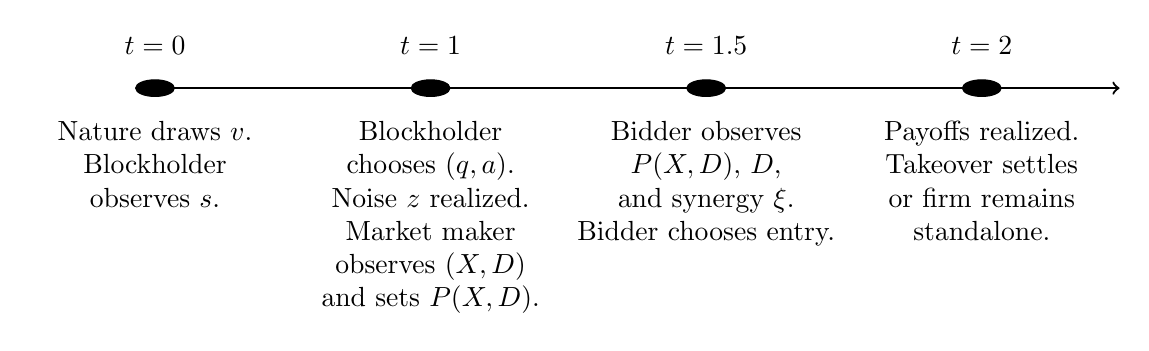
\begin{tikzpicture}[xscale=3.5, yscale=1.5]
    % Draw timeline line
    \draw[thick, ->] (0,0) -- (3.5,0);

    % Draw nodes
    \filldraw (0,0) circle (2pt);
    \filldraw (1,0) circle (2pt);
    \filldraw (2,0) circle (2pt);
    \filldraw (3,0) circle (2pt);

    % Draw time labels
    \node[above, font=\bfseries] at (0,0.2) {$t = 0$};
    \node[above, font=\bfseries] at (1,0.2) {$t = 1$};
    \node[above, font=\bfseries] at (2,0.2) {$t = 1.5$};
    \node[above, font=\bfseries] at (3,0.2) {$t = 2$};

    % Draw descriptions
    \node[below, align=center, text width=3cm] at (0,-0.2) {Nature draws $v$.\\Blockholder observes $s$.};
    \node[below, align=center, text width=3.5cm] at (1,-0.2) {Blockholder chooses $(q,a)$.\\Noise $z$ realized.\\Market maker observes $(X,D)$ and sets $P(X,D)$.};
    \node[below, align=center, text width=3.5cm] at (2,-0.2) {Bidder observes $P(X,D)$, $D$, and synergy $\xi$.\\Bidder chooses entry.};
    \node[below, align=center, text width=3cm] at (3,-0.2) {Payoffs realized.\\Takeover settles or firm remains standalone.};
\end{tikzpicture}
\caption{Timeline of the model. The four stages capture the blockholder's information advantage, the market's inference problem, and the bidder's response.}
\label{fig:timeline}
\end{figure}

Table~\ref{tab:notation} in Appendix~\ref{app:notation} provides a quick reference for notation. The remainder of this section introduces each model component in turn, beginning with the blockholder's information environment and ending with the equilibrium concept.

%
\subsection{Fundamentals and Information}
%

The standalone fundamental is $v \sim \mathcal{N}(\mu, \sigma_v^2)$. The blockholder observes a private signal
\[
s = v + \varepsilon, \quad \varepsilon \sim \mathcal{N}(0, \sigma_\varepsilon^2),
\]
independent of $v$. Let $\sigma_s^2 \equiv \sigma_v^2 + \sigma_\varepsilon^2$. The blockholder's posterior mean is linear:
\[
\hat{v}(s) \equiv \E[v \mid s] = \mu + \beta(s - \mu), \quad \beta \equiv \frac{\sigma_v^2}{\sigma_v^2 + \sigma_\varepsilon^2} \in (0,1).
\]

The bidder draws an independent synergy shock $\xi \sim \mathcal{N}(0, \sigma_\xi^2)$. This signal structure gives the blockholder a transient information advantage that she can exploit through trading, engagement, or both.

%
\subsection{Trading and Liquidity}
%

The blockholder has an initial stake of one share (normalization). Her order $q \in \{-1, 0, +1\}$ implies an end-of-$t=1$ holding of $h = 1 + q$ shares.

Noise trading is discrete:
\[
z \in \{-1, 0, 1\}, \quad \PP(z = 0) = 1 - \kappa, \quad \PP(z = \pm 1) = \kappa/2,
\]
where $\kappa \in (0, 1)$ indexes noise-trading intensity (market liquidity). Higher $\kappa$ means more frequent nonzero noise imbalance and therefore weaker inference from order flow.

Total order flow observed by the market maker is
\[
X = q + z \in \{-2, -1, 0, 1, 2\}.
\]

The blockholder's trading decision is intertwined with her engagement choice, to which I now turn.

%
\subsection{Disclosure Rule}
%

Let $D \in \{0, 1\}$ be a public indicator for whether a stake acquisition crosses a disclosure threshold. I model disclosure as \emph{stake-triggered}: in the discrete framework,
\[
D = 1 \quad \Longleftrightarrow \quad (q = +1).
\]
That is, \textbf{if the blockholder acquires an additional share, a threshold-crossing disclosure occurs}. This captures the institutional logic that crossing an ownership threshold triggers a regulatory filing (e.g., Schedule 13D), independent of whether the filing explicitly reflects intent. Below-threshold engagement remains hidden.

\paragraph{Timing of disclosure.} The disclosure indicator $D$ is determined simultaneously with the blockholder's action $(q, a)$ and is observed by the market maker at the same time as order flow $X$. Specifically, the sequence within $t=1$ is:
\begin{enumerate}[label=(\roman*),leftmargin=2em,itemsep=0pt]
\item The blockholder chooses $(q, a)$, which determines $D = \1\{q=+1\}$.
\item Noise trader submits $z$; total order flow $X = q + z$ is realized.
\item The market maker observes $(X, D)$ jointly and sets price $P(X, D)$.
\end{enumerate}
This timing ensures that disclosure does not reveal additional information beyond what is captured by $(X, D)$ jointly.

%
\subsection{Engagement Technology (Voice)}
\label{sec:engagement}
%

If the blockholder chooses engagement $a = 1$, she pays a private, signal-dependent cost $C(s) > 0$ at $t = 1$. This cost is observed by the blockholder when she observes $s$ but not by the market maker or bidder. I assume engagement costs are decreasing in the signal: a blockholder with more favorable private information finds it easier to build a compelling case for change. I parameterize the cost as
\[
C(s) = C_0 \exp\!\left(-\chi \frac{s - \mu}{\sigma_s}\right),
\]
where $C_0 > 0$ is the cost at the prior mean and $\chi \geq 0$ controls cost sensitivity to signal quality (Assumption~\textup{(A2)}). The assumption that engagement costs are decreasing in the signal reflects the economic mechanics of persuasion. A blockholder with more favorable private information about fundamentals finds it easier to build a compelling case for change. With a strong underlying asset, the activist can point to concrete operational improvements, favorable peer comparisons, or verifiable evidence of undervaluation, substantially lowering the friction of persuading the board or rallying fellow institutional shareholders. The exponential form is chosen for analytical convenience to ensure non-negativity, but the qualitative results require only strict positivity and a monotone decrease in $s$. This monotonicity assumption is economically substantive. If costs were instead increasing in $s$ (for example, because high-value firms feature entrenched managers who are harder to dislodge), the cutoff ordering would potentially invert, pushing the blockholder toward exit on good news and voice on bad news. The decreasing cost structure captures the standard paradigm where a strong fundamental thesis is required for a viable activist campaign.

The decreasing-cost assumption~\textup{(A2)} is \emph{sufficient but not necessary} for the model's qualitative architecture. As shown in Appendix~\ref{app:d5}, the four-action threshold ordering $k_1\le k_0\le k_D$ survives \emph{any} cost profile in the \emph{persuasion regime} $C'(s)<\Lambda(s)$, where $\Lambda(s)$ is the gross (pre-cost) Quiet-over-Hold value slope (Proposition~\ref{prop:d5-a2}); this includes a flat cost ($\chi=0$), under which all existence, ordering, and comparative-statics results go through unchanged and only the \emph{level} of the Hold/Quiet boundary $k_0$ shifts. The ordering can invert only under an \emph{entrenchment regime} ($C'(s)\ge\Lambda(s)$ on a nondegenerate set, e.g.\ better-informed blockholders facing harsher managerial entrenchment precisely when their case is strong), which carries the opposite, falsifiable empirical signature (Definition~\ref{def:d5-regimes}, Remark~\ref{rem:d5-mech}). The single role of $\chi>0$ is therefore not qualitative existence but \emph{magnitude}: a decreasing cost tilts engagement toward higher-signal types. The interior peak of $\Delta^{\min}(\kappa)$ likewise survives a flat cost, with endpoint symmetry $\Delta^{\min}(0^+)=\Delta^{\min}(1^-)$ derived from the noise law (Appendix~\ref{app:d5}).

This monotone, strictly positive specification ensures that neither engagement nor passivity is always optimal when the blockholder holds her initial stake, yielding an interior cutoff structure (Assumption~\textup{(A1)}).%
\footnote{Sufficient conditions for interior cutoffs include $C(\mu) < \delta(\tilde{\Delta} + (\tilde{m}-m_0))$ (engagement is worthwhile at the prior mean) and $\lim_{s\to-\infty} C(s) > \delta(\tilde{\Delta} + (\tilde{m}-m_0))$ (engagement is dominated for sufficiently low signals), together with the monotonicity of $C(s)$. I also assume that stake building (Public Voice) is not always dominated when engagement occurs, so that disclosure is triggered for sufficiently high signals. When $\chi > 0$, cost heterogeneity supports an interior Hold region; when $\chi = 0$, costs are constant and the equilibrium collapses to the two-cutoff case.}

Engagement succeeds with probability $\rho \in (0,1]$ and affects outcomes in two ways when successful:

\paragraph{Outside option improvement.} If engagement succeeds and no takeover is consummated, the standalone payoff is increased by $\Delta > 0$ at $t=2$. If engagement fails, standalone payoff remains $v$.

\paragraph{Bargaining/resistance premium.} If engagement succeeds and a takeover is consummated, the required premium increases from $m_0$ to $m_1$, where $m_1 > m_0 \geq 0$. The wedge captures bargaining power, defensive tactics, or any friction that raises the price needed to complete the acquisition when an engaged blockholder is present. Failed engagement yields the baseline premium $m_0$.
I interpret $m_0$ and $m_1$ as \emph{per-share takeover premia} above the market price (so the consummated offer satisfies $b=P+m$); they are distinct from $\hat{v}(s)$, the posterior mean of fundamentals.

\paragraph{Risk-neutral simplification.} Since success is unobserved before $t=2$ and all parties are risk-neutral, I define expected engagement effects:
\[
\tilde{\Delta} \equiv \rho \Delta, \qquad \tilde{m} \equiv m_0 + \rho(m_1 - m_0).
\]
Then engagement ($a=1$) yields expected standalone improvement $\tilde{\Delta}$ and expected premium wedge $\tilde{m}$. I assume the premium wedge satisfies $\tilde{m} > m_0$, which requires $\rho(m_1 - m_0) > 0$ (Assumption~\textup{(A3)}). This ensures that engagement has real consequences for takeover outcomes; an engaged blockholder can extract higher premia through an improved bargaining position or defensive tactics.

\paragraph{Bargaining micro-foundation of the premium wedge.} Assumption~\textup{(A3)} can be read as the conclusion of an explicit bargaining stage rather than a free-standing primitive. In Appendix~\ref{app:bg} I show that if the bid-conditional premia $(m_0,m_1)$ arise from generalized Nash bargaining between the target's control bloc (bargaining weight $\theta\in(0,1)$) and the bidder over the takeover surplus $\bar S+\xi$, and if engagement raises the bloc's disagreement payoff by an appropriable amount $\lambda\,\rho\,\Delta_{\mathrm{eng}}>0$ (Condition~\ref{cond:bg}, motivated by the free-rider tender logic of \citet{GrossmanHart1980} and the outside-option reading of \citet{BinmoreRubinsteinWolinsky1986}), then the wedge is the closed form $m_1-m_0=(1-\theta)\lambda\rho\Delta_{\mathrm{eng}}$, which is invariant to the synergy draw $\xi$, and $\tilde m>m_0$ follows as a theorem whenever $\theta<1$ (Theorem~\ref{thm:bg-A3}). The reduced form used in the body is exactly the constant-$\theta$, full-appropriability ($\lambda=1$) special case; the appendix is explicit about what is proved (the Nash split, the wedge's $\xi$-invariance, the reduced-form nesting) versus what remains a transparent structural condition (the appropriability coefficient $\lambda$, which a complete tender-game equilibrium would be needed to derive).

%
\subsection{Bidder Entry and Bidding Terms}
%

The bidder follows a price-contingent entry rule as in standard takeover models \citep{GrossmanHart1980,Fishman1988,BulowHuangKlemperer1999,EdmansGoldsteinJiang2012}. The bidder observes the public pair $(P(X,D), D)$ and a private synergy shock $\xi$. On the nondisclosed branch $D=0$, I assume the equilibrium price schedule separates order-flow realizations ($P^*(X,0) \neq P^*(X',0)$ for all distinct $X, X' \in \{-2,-1,0,1\}$) so that the bidder can infer $X$ from $(P,0)$ (Assumption~\textup{(A7)}).%
\footnote{Injectivity on the $D=0$ branch is a standard regularity condition in discrete-order-flow models: different $X$ imply different posteriors about fundamentals and hence different competitive prices. Assumption~\textup{(A7)} avoids a notational distinction between conditioning on $(P,D)$ and conditioning on $(X,D)$.}
I therefore use $p(X,0)$ and $\bar{m}(X,0)$ as shorthand for $p(P(X,0),0)$ and $\bar{m}(P(X,0),0)$. On the disclosed branch $D=1$, disclosure pins down Public Voice and hence $a=1$, so $X$ reveals only the noise realization and carries no information about fundamentals. Under Assumption~A5 (described below), this implies that equilibrium beliefs and the pricing fixed point are identical across $X\in\{0,1,2\}$ on the disclosed branch, so $P^*(X,1)$ and $p(X,1)$ are constant across $X$ (see Appendix~\ref{app:proof-disclosed-invariance}). I therefore continue to write $p(X,1)$ as shorthand for $p(P^*(X,1),1)$.

I assume that synergies and costs satisfy $\bar{S}-K > m_0-\mu$ and $\bar{S}-K < m_1+(\mu+3\sigma_v)$ (Assumption~\textup{(A4)}). These bounds ensure that takeover bids occur with interior probability: the bidder is neither always deterred nor always willing to bid regardless of prices.

Conditional on $(P,D)$, the bidder's net deal surplus is
\[
\Pi_B(X,D) = \bar{S} - P(X,D) + \xi - \bar{m}(X,D) - K,
\]
where $\bar{S}$ is baseline synergy, $K > 0$ is a fixed bidding cost, and $\bar{m}(X,D)$ is the expected premium wedge conditional on $(X,D)$. The market price enters surplus dollar-for-dollar because the bidder must pay the target's market value (plus the premium wedge) to complete the acquisition.

The premium wedge ultimately depends on whether the blockholder has engaged. I define the premium required to complete the acquisition as a function of the \emph{realized} engagement action $a$:
\[
m^{R}(a) \equiv m_0 + a\cdot(\tilde{m}-m_0), \qquad a\in\{0,1\}.
\]
I interpret $m^{R}(a)$ as the (ex ante) premium required at closing, determined by the blockholder's engagement-driven resistance.
When engagement is not publicly disclosed, the market maker and bidder do not observe $a$ and instead form the posterior $\pi(X,D)=\PP(a=1 \mid X,D)$. The corresponding \emph{expected} premium wedge conditional on $(X,D)$ is therefore
\[
\bar{m}(X,D) \equiv \E[m^{R}(a) \mid X,D] = m_0 + (\tilde{m} - m_0)\cdot \pi(X,D), \quad \pi(X,D) \equiv \PP(a = 1 \mid X, D).
\]

I define $\bar{m}(P,D)\equiv \bar{m}(X(P,D),D)$ and the takeover completion probability conditional on observed $(P,D)$ as
\begin{equation}
p(P,D) \equiv 1 - \Phi\left(\frac{\bar{m}(P,D) + K - \bar{S} + P}{\sigma_\xi}\right),
\label{eq:bid-prob}
\end{equation}
and use the shorthand $p(X,D)\equiv p(P(X,D),D)$ in equilibrium. The bidder initiates a takeover attempt if and only if $\Pi_B(X,D) \geq 0$, so $p(P,D)$ is the probability of a consummated transaction.
Here $\Phi(\cdot)$ is the standard normal cumulative distribution function.

If the takeover is consummated, the \emph{realized} per-share offer is
\[
b(X,D,a) = P(X,D) + m^{R}(a).
\]

%
\subsection{Terminal Payoff and Price Formation}
%

Let $\delta = \exp(-r\tau)$ (approximately $1/(1+r)$ for short horizons) be the discount factor between the pricing/entry date and payoff/settlement at $t=2$, where $\tau$ is the time between these dates \citep{Cochrane2005,Duffie2010}.%
\footnote{If one measures payoffs in time-$1$ present-value units, $\delta$ can be set to one and later reintroduced by scaling. I keep $\delta$ explicit throughout.}

If no takeover is consummated, per-share terminal payoff is $y^{\text{stand}} = v + a\tilde{\Delta}$. If a takeover is consummated, per-share payoff is $y^{\text{M\&A}} = b(X,D,a) = P(X,D) + m^{R}(a)$.

Therefore, the per-share terminal payoff is
\[
Y = \1\{\textup{bid}\} \cdot (P(X,D) + m^{R}(a)) + (1 - \1\{\textup{bid}\}) \cdot (v + a\tilde{\Delta}),
\]
where $\1\{\textup{bid}\}$ denotes a \emph{consummated} takeover rather than a mere offer. Bargaining, board resistance, and regulatory frictions are captured in reduced form by the premium wedge $m^{R}(\cdot)$ and the fixed cost $K$. A simple robustness extension would multiply $p(P,D)$ by a completion probability $\alpha(P,D)\in(0,1]$ in the pricing fixed point, without altering the main mechanism.

Conditional on $(X,D)$, $\E[m^{R}(a) \mid X,D]=\bar{m}(X,D)$, so the expected takeover payoff equals $P(X,D)+\bar{m}(X,D)$; this keeps the pricing fixed-point equations below unchanged.

The market maker is competitive and sets
\begin{equation}
P(X,D) = \delta \, \E[Y \mid X, D].
\label{eq:pricing}
\end{equation}

Equation~\eqref{eq:pricing} is the key equilibrium discipline: the price reflects the possibility of takeover and the premium wedge, and takeover decisions depend on that same price. I assume that for each information set $(X,D)$ and each feasible posterior $\pi(X,D)$, the competitive pricing fixed point admits a unique solution $P^*(X,D)$, and that takeover entry is not too sensitive to prices: $\delta\cdot\sup_P|\partial p/\partial P|<1$ (Assumption~\textup{(A5)}).%
\footnote{Assumption~\textup{(A5)} bounds the strength of the price-to-entry feedback loop and ensures that comparative statics are well-defined. Under the Gaussian bidding rule, a sufficient condition is $\delta/\sigma_\xi < 1/\phi(0)$, where $\phi(\cdot)$ is the standard normal density.}

%
\subsection{Blockholder Payoff and Equilibrium Concept}
%

Conditional on signal $s$, the blockholder chooses $(q, a)$ to maximize expected present value. If she submits $q$ and ends with $h = 1 + q$ shares, her $t = 1$ value is
\[
U(q, a \mid s) = \E\Big[-q \cdot P(X,D) + \delta \cdot h \cdot Y - a \cdot C(s) \,\Big|\, s, q, a\Big],
\]
where $-qP(X,D)$ is the net cash flow from trading at $t = 1$ (selling $q = -1$ yields $+P$; buying $q = +1$ yields $-P$).

\begin{definition}[Perfect Bayesian Equilibrium]
A \emph{Perfect Bayesian Equilibrium} consists of:
\begin{enumerate}[label=(\roman{enumi})]
\item a blockholder strategy mapping $s$ into $(q, a)$,
\item beliefs $\pi(X,D) = \PP(a = 1 \mid X, D)$ consistent with Bayes' rule,
\item a bidder entry strategy satisfying~\eqref{eq:bid-prob}, and
\item a competitive price schedule $P(X,D)$ satisfying~\eqref{eq:pricing}.
\end{enumerate}
\end{definition}

Because noise trading $z$ has full support on $\{-1,0,+1\}$, every $(X,D)$ pair that is feasible under an on-path action occurs with positive probability. In particular, when $D=0$, $X\in\{-2,-1,0,1\}$; when $D=1$, only Public Voice is feasible so $X\in\{0,1,2\}$. Consequently, Bayes' rule pins down $\pi(X,D)$ for all reached information sets; off-path beliefs are irrelevant.%
\footnote{Throughout, I maintain Assumptions~\textup{(A1)}--\textup{(A7)} (the Standing Assumptions). These ensure interior action regions, nontrivial takeover outcomes, and well-behaved equilibrium existence. I verify each assumption numerically in the baseline calibration. Assumption~\textup{(A6)} (contraction) ensures uniqueness of the monotone-cutoff equilibrium; existence is established unconditionally via Brouwer's theorem (Proposition~\ref{prop:existence}), while uniqueness is verified numerically following \citet{EdmansGoldsteinJiang2015}.}
%==============================================================================
\section{Equilibrium Characterization}
\label{sec:equilibrium}
%==============================================================================

%
\subsection{Threshold Structure with Three Cutoffs}
%

The blockholder's optimal strategy has a natural ordering: she exits on bad news, holds passively on mildly negative news, engages quietly on moderate news, and goes public on good news. The next result makes this precise.

\begin{proposition}[Monotone Cutoff Structure]
\label{prop:cutoffs}
Under the Standing Assumptions, there exists a Perfect Bayesian Equilibrium in which the blockholder follows cutoff rules with (weakly) ordered thresholds $k_1 \leq k_0 \leq k_D$:
\[
(q, a) = \begin{cases}
(-1, 0) & s < k_1 \quad \text{(Exit)}, \\
(0, 0) & k_1 \leq s < k_0 \quad \text{(Hold)}, \\
(0, 1) & k_0 \leq s < k_D \quad \text{(Quiet Voice)}, \\
(+1, 1) & s \geq k_D \quad \text{(Public Voice)}.
\end{cases}
\]
The corresponding disclosure outcomes are: $D = 1$ if and only if $q = +1$ (Public Voice), and $D = 0$ otherwise.
\end{proposition}
\textit{Proof.} See Appendix~\ref{app:proof-cutoffs}.

The ordering reflects how the blockholder's incentives shift with her private signal. For very low signals, she holds unfavorable information about fundamentals and prefers to sell, monetizing her negative information before it reaches prices.

For somewhat better signals, fundamentals are not bad enough to warrant selling at a discount, but engagement is not yet worthwhile given its cost. The blockholder holds passively.

For intermediate signals, engagement improves expected value enough to justify the campaign cost $C(s)$, but stake building remains unattractive: buying additional shares costs more than the benefit of higher ownership. The blockholder engages quietly.

For the highest signals, buying additional shares allows the blockholder to internalize more of the engagement gains, and the discrete stake increase triggers public disclosure. This is the Public Voice region.

When engagement costs are constant (i.e., $\chi=0$), the Hold region may collapse, yielding a simpler two-cutoff structure with $k_0=k_1$. The analysis accommodates this case by allowing weak inequalities among cutoffs.

%
\subsection{Action Probabilities}
%

Given cutoffs $(k_1, k_0, k_D)$, define standardized cutoffs $\alpha_i \equiv (k_i - \mu)/\sigma_s$ for $i \in \{1, 0, D\}$. The unconditional action probabilities are:
\begin{align*}
\omega_E &\equiv \PP(s < k_1) = \Phi(\alpha_1), \\
\omega_H &\equiv \PP(k_1 \leq s < k_0) = \Phi(\alpha_0) - \Phi(\alpha_1), \\
\omega_Q &\equiv \PP(k_0 \leq s < k_D) = \Phi(\alpha_D) - \Phi(\alpha_0), \\
\omega_P &\equiv \PP(s \geq k_D) = 1 - \Phi(\alpha_D),
\end{align*}
corresponding to Exit, Hold, Quiet Voice, and Public Voice.

%
\subsection{Conditional Means of Fundamentals}
%

Let $\lambda_L(\alpha) \equiv \phi(\alpha)/\Phi(\alpha)$ and $\lambda_U(\alpha) \equiv \phi(\alpha)/(1-\Phi(\alpha))$ denote inverse Mills ratios. The conditional means of $v$ in each signal region are:
\begin{align*}
\mu_E &\equiv \E[v \mid s < k_1] = \mu - \beta\sigma_s \lambda_L(\alpha_1), \\
\mu_H &\equiv \E[v \mid k_1 \leq s < k_0] = \mu + \beta\sigma_s \frac{\phi(\alpha_1) - \phi(\alpha_0)}{\Phi(\alpha_0) - \Phi(\alpha_1)}, \\
\mu_Q &\equiv \E[v \mid k_0 \leq s < k_D] = \mu + \beta\sigma_s \frac{\phi(\alpha_0) - \phi(\alpha_D)}{\Phi(\alpha_D) - \Phi(\alpha_0)}, \\
\mu_P &\equiv \E[v \mid s \geq k_D] = \mu + \beta\sigma_s \lambda_U(\alpha_D).
\end{align*}

%
\subsection{Bayesian Posteriors}
%

Disclosure creates a sharp asymmetry in what the market can learn: when activism is disclosed, inference is trivial; when it is not, the market must extract engagement probabilities from noisy order flow. The next result characterizes the posterior beliefs that sustain equilibrium pricing.

\begin{proposition}[Posterior Engagement Probabilities]
\label{prop:posteriors}
For any information set $(X,D)$ that is reached with positive probability in equilibrium, the posterior probability of engagement $\pi(X,D) = \PP(a=1 \mid X, D)$ satisfies:
\begin{enumerate}[label=(\alph*)]
\item \textbf{Disclosed states:} If $D = 1$, then $\pi(X, 1) = 1$ for all compatible $X \in \{0, 1, 2\}$.
\item \textbf{Nondisclosed states:} If $D = 0$, let $p_0 \equiv 1 - \kappa$ and $p_1 \equiv \kappa/2$. Then:
\begin{align*}
\pi(1, 0) &= \frac{\omega_Q}{\omega_H + \omega_Q}, \\
\pi(-1, 0) &= \frac{\omega_Q \, p_1}{(\omega_H + \omega_Q) \, p_1 + \omega_E \, p_0}, \\
\pi(0, 0) &= \frac{\omega_Q \, p_0}{(\omega_H + \omega_Q) \, p_0 + \omega_E \, p_1}, \\
\pi(-2, 0) &= 0.
\end{align*}
\end{enumerate}
\end{proposition}
\textit{Proof.} See Appendix~\ref{app:proof-posteriors}.

When $D=1$, the inference problem collapses entirely: disclosure reveals that the blockholder chose Public Voice, which implies engagement with certainty. The market knows activism has occurred, though the ultimate success of the campaign remains uncertain until $t=2$.

When $D=0$, the market faces a genuine inference problem. It observes only aggregate order flow $X$ and must form beliefs about whether the blockholder is engaged (Quiet Voice) or not (Exit or Hold). The key insight is that Hold and Quiet Voice both involve $q=0$, so they generate identical order-flow distributions; the market cannot distinguish between them from order flow alone. Instead, the posterior split between these actions is pinned down by their prior probabilities $(\omega_H,\omega_Q)$, which depend on the equilibrium cutoffs.

This is where liquidity enters the inference channel: higher $\kappa$ changes the noise distribution and thereby affects how order flow $X$ is interpreted. The posteriors $\pi(X,0)$ inherit this liquidity dependence, transmitting it to prices and takeover premia.

%
\subsection{Conditional Expectation of Fundamentals Given \texorpdfstring{$(X,D)$}{(X,D)}}
%

For pricing, we need $\E[v \mid X, D]$. Since $v$ is independent of noise $z$, only the action regions compatible with $(X, D)$ matter.

\paragraph{For $D=1$:} Only Public Voice is possible:
\[
\E[v \mid X, D=1] = \mu_P \quad \text{for } X \in \{0, 1, 2\}.
\]

\paragraph{For $D=0$:} Mix over Exit, Hold, and Quiet Voice with Bayesian weights. Let $p_0 \equiv 1 - \kappa$ and $p_1 \equiv \kappa/2$. Then:
\begin{align*}
\E[v \mid -2, 0] &= \mu_E, \\
\E[v \mid 1, 0] &= \frac{\omega_H \mu_H + \omega_Q \mu_Q}{\omega_H + \omega_Q}, \\
\E[v \mid -1, 0] &= \frac{(\omega_H \mu_H + \omega_Q \mu_Q) \, p_1 + \omega_E \mu_E \, p_0}{(\omega_H + \omega_Q) \, p_1 + \omega_E \, p_0}, \\
\E[v \mid 0, 0] &= \frac{(\omega_H \mu_H + \omega_Q \mu_Q) \, p_0 + \omega_E \mu_E \, p_1}{(\omega_H + \omega_Q) \, p_0 + \omega_E \, p_1}.
\end{align*}

%
\subsection{Equilibrium Prices}
\label{sec:prices}
%

The competitive pricing condition~\eqref{eq:pricing} defines $P(X,D)$ implicitly, since the bid probability $p(X,D)$ depends on $P(X,D)$ through~\eqref{eq:bid-prob}. For each information set $(X,D)$ and posterior $\pi(X,D)$, the equilibrium price $P^*(X,D)$ satisfies
\begin{equation}
P = \delta\Big((1-p(P,D)) \cdot \hat{V}(X,D) + p(P,D) \cdot (P + \bar{m}(X,D))\Big),
\label{eq:price-fp}
\end{equation}
where $\hat{V}(X,D) \equiv \E[v \mid X,D] + \tilde{\Delta} \cdot \pi(X,D)$ is the expected standalone value (including engagement effects), and $p(P,D) = 1 - \Phi\big((\bar{m}(P,D) + K - \bar{S} + P)/\sigma_\xi\big)$ is the bid probability. Under Assumption~\textup{(A5)}, this fixed-point equation admits a unique solution for each $(X,D)$.

The fixed-point structure captures a key economic feedback: the price depends on takeover probability, which in turn depends on price. Higher prices deter bidders (making takeover less likely), which reduces the takeover component of value, which feeds back into the price. Assumption~\textup{(A5)} ensures that this feedback loop does not generate multiplicity.

Rearranging~\eqref{eq:price-fp}, any fixed point satisfies
\[
P^*(X,D)=\frac{\delta\big((1-p^*)\hat{V}(X,D)+p^*\,\bar{m}(X,D)\big)}{1-\delta p^*},
\qquad p^*\equiv p(P^*(X,D),D).
\]
When takeover is unlikely ($p^*\approx 0$), this reduces to $P^*(X,D)\approx \delta\,\hat{V}(X,D)$.

%
\subsection{Price Decomposition and Activism Premium}
%

Building on the pricing fixed point~\eqref{eq:price-fp}, I decompose the equilibrium price into interpretable components. The decomposition isolates the channels through which blockholder engagement feeds into asset prices.

\begin{proposition}[Price Decomposition]
\label{prop:price-decomp}
The unique equilibrium price $P^*(X,D)$ satisfies
\[
P^*(X,D) = \delta\Big((1-p^*) \cdot \E[v \mid X,D] + (1-p^*) \cdot \tilde{\Delta} \cdot \pi(X,D) + p^* \cdot (P^*(X,D) + \bar{m}(X,D))\Big),
\]
where $p^* \equiv p(P^*(X,D),D)$, $\pi(X,D) = \PP(a=1 \mid X,D)$, and $\bar{m}(X,D) = m_0 + (\tilde{m} - m_0)\pi(X,D)$.

The terms involving $\pi(X,D)$ constitute an ``activism premium'':
\begin{itemize}[leftmargin=1.5em,itemsep=0pt]
\item \textbf{Standalone channel:} $(1-p^*)\tilde{\Delta}\pi(X,D)$ reflects expected value improvement from engagement when no takeover occurs.
\item \textbf{Takeover channel:} $p^* \cdot (\tilde{m}-m_0)\pi(X,D)$ reflects the expected \emph{incremental} takeover premium attributable to engagement (over and above the baseline $m_0$).
\end{itemize}
\end{proposition}
\textit{Proof.} See Appendix~\ref{app:proof-price-decomp}.

Activism affects prices through two distinct channels. The \emph{standalone channel} operates when no takeover occurs: an engaged blockholder improves firm value by $\tilde{\Delta}$ in expectation, and this improvement is capitalized into the share price.

The \emph{takeover channel} operates when a bid arrives: the bidder must pay a higher premium to acquire a firm with an engaged blockholder, and this higher premium is also reflected in the pre-bid price.

The way these channels operate differs sharply between disclosed and nondisclosed states. In disclosed states ($D=1$), engagement is known with certainty, so $\pi(X,1)=1$ and the activism premium is fully priced. Liquidity affects how often $D=1$ occurs and can influence prices through feedback, but it does not affect the activism premium \emph{within} disclosed states.

In nondisclosed states ($D=0$), the posterior $\pi(X,0)$ depends on $\kappa$ through Bayesian inference, so the activism premium inherits liquidity sensitivity. This asymmetry between disclosed and nondisclosed states is central to understanding how disclosure attenuates the liquidity--premia relationship.

%
\subsection{Bid Incidence and Premia}
%

The bid probability $p(X,D)$ defined in~\eqref{eq:bid-prob} has two key monotonicity properties. First, higher prices deter bids: $\partial p(X,D)/\partial P(X,D)<0$. This is intuitive: a higher market price raises the acquisition cost and makes the deal less attractive to the bidder.

Second, when the activism premium is positive ($\tilde{m}>m_0$), higher inferred engagement also reduces bid incidence: $\partial p(X,D)/\partial\pi(X,D)<0$. The bidder anticipates paying a higher premium when facing an engaged blockholder, which makes entry less attractive.

These monotonicity properties have a direct implication for the role of disclosure. When $D=1$, the bidder \emph{knows} activism has occurred, so bid deterrence is maximal: the full activism premium $\tilde{m}$ enters the bidder's calculation. When $D=0$, deterrence is probabilistic and depends on the inferred engagement probability $\pi(X,0)$. Consequently, disclosed activism deters bids more strongly than inferred activism, all else equal. (Proof: see Appendix~\ref{app:proof-bid-monotone}.)

%
\subsection{Equilibrium Cutoff Equations}
%

The equilibrium cutoffs $(k_1,k_0,k_D)$ are pinned down by indifference conditions at each boundary. Let $U_E$, $U_H(s)$, $U_Q(s)$, and $U_P(s)$ denote the expected payoffs from Exit, Hold, Quiet Voice, and Public Voice, computed by integrating over noise realizations and disclosure outcomes. (The exit payoff $U_E$ does not depend on $s$ because the sell order $q=-1$ fully liquidates the position, so the blockholder's terminal holding is zero.) The three cutoffs satisfy:
\begin{align}
U_E &= U_H(k_1), \label{eq:k1} \\
U_H(k_0) &= U_Q(k_0), \label{eq:k0} \\
U_Q(k_D) &= U_P(k_D). \label{eq:kD}
\end{align}

At $k_1$, the blockholder is indifferent between exiting and holding passively. At $k_0$, she is indifferent between Hold and Quiet Voice. At $k_D$, she is indifferent between Quiet Voice and Public Voice. These indifference conditions, combined with single-crossing of payoffs in the signal $s$, pin down the equilibrium strategy. (Derivation: see Appendix~\ref{app:proof-cutoff-eqns}.)

%
\subsection{Equilibrium Existence and Uniqueness}
%

Under Assumptions~\textup{(A1)}--\textup{(A5)}, any monotone-cutoff Perfect Bayesian Equilibrium must satisfy Bayes-consistent beliefs and the pricing fixed point~\eqref{eq:price-fp} together with the cutoff indifference conditions~\eqref{eq:k1}--\eqref{eq:kD}.

A pure strategy for the blockholder partitions the signal line into the four action regions by an ordered triple of cutoffs. Fix a finite bracket $[\underline{s},\overline{s}]$ containing all indifference points (its existence is established in Lemma~\ref{lem:bounded}) and define the \emph{cutoff polytope}
\begin{equation}
\label{eq:theta}
\Theta \;=\; \bigl\{\, \kvec=(\kone,\kzero,\kD)\in[\underline{s},\overline{s}]^3
\;:\; \underline{s}\le \kone \le \kzero \le \kD \le \overline{s}\,\bigr\}.
\end{equation}
$\Theta$ is the intersection of a cube with the half-spaces $\{\kone\le\kzero\}$ and $\{\kzero\le\kD\}$, hence a compact, convex, nonempty polytope. The boundary faces $\{\kone=\kzero\}$ and $\{\kzero=\kD\}$ are \emph{collapse faces} on which Hold (respectively Quiet Voice) carries zero probability; the baseline equilibrium lives on the face $\kone=\kzero$ (Hold collapses).

The best-response map $\Tmap:\Theta\to\R^3$ sends a conjecture $\kvec$ to the indifference cutoffs it implies. Given $\kvec$, the market maker's pricing function $P(\cdot,\cdot)$ and the bidder's takeover probability $p(\cdot)$ are determined, and the blockholder's payoff to action $(q,a)$ at signal $s$ is, from \eqref{eq:U-affine},
\begin{equation}
\label{eq:payoff-affine}
U(q,a;s) \;=\; A(q,a)\;+\; B(q,a)\,\vhat(s)\;-\;a\,\Ccost(s),
\end{equation}
where, writing $\beta=\sv^2/\sigma_s^2\in(0,1]$ for the posterior-mean slope and absorbing the conjecture into the intercepts $A(\cdot)$,
\begin{equation}
\label{eq:slopes}
B(E)\;=\;0,\qquad B(H)\;=\;1,\qquad B(Q)\;=\;1,\qquad B(P)\;=\;1+\eta,
\quad \eta>0,
\end{equation}
the extra slope $\eta$ on Public Voice arising from the trading term $q[\Vhat-P]$ with $q=+1$ (the price-taking blockholder takes $P$ as given, so trading contributes a slope of $+1$ in $\vhat$) and from the takeover term, which is nondecreasing in $\vhat$ (Lemma~\ref{lem:BP-BQ}). The component $\Tmap_1$ ($\Tmap_2$, $\Tmap_3$) is the Exit/Hold (Hold/Quiet, Quiet/Public) indifference signal.

\begin{lemma}[Boundedness of best responses]
\label{lem:bounded}
Under Assumptions~\textup{(A1)}, \textup{(A2)}, \textup{(A4)}, there is a finite bracket $[\underline{s},\overline{s}]$, independent of the conjecture $\kvec\in\Theta$, such that every indifference signal of $\Tmap$ lies in $[\underline{s},\overline{s}]$.
\end{lemma}

\begin{proof}
Each indifference condition equates two payoffs of the form \eqref{eq:payoff-affine}. The difference between two such payoffs is
\begin{equation}
\label{eq:diff}
D_{ab}(s)=\bigl[A(a)-A(b)\bigr]+\bigl[B(a)-B(b)\bigr]\vhat(s)
-\bigl[\1\{a\in\{Q,P\}\}-\1\{b\in\{Q,P\}\}\bigr]\Ccost(s).
\end{equation}
The intercepts $A(\cdot)$ are bounded uniformly over $\kvec\in\Theta$: prices lie in $[\,0,\deltaliq\,\overline{Y}\,]$ with $\overline{Y}$ the finite maximal terminal value, and the takeover probability $p\in[0,1]$. The slope gap $B(a)-B(b)$ is one of $\{\pm1,\pm\eta,\pm(1+\eta)\}$ and is nonzero for every adjacent pair $(E,H),(H,Q),(Q,P)$ except $(H,Q)$, treated separately. For a nonzero slope, $\vhat(s)=\mu+\beta(s-\mu)\to\pm\infty$ as $s\to\pm\infty$, while $\Ccost(s)=C_0\exp(-\chivar(s-\mu)/\sigma_s)$ is bounded on the half-line where $\vhat$ dominates: as $s\to+\infty$ the linear term forces $D_{ab}\to+\infty$ for the higher-slope action; in the $(E,H)$ comparison the cost term is absent, and in the $(Q,P)$ comparison the common engagement cost cancels, so the slope gap $\eta>0$ on $\vhat$ governs the crossing, which is finite. The $(H,Q)$ comparison has $B(H)=B(Q)$ and reduces to $\Ccost(s)=A(Q)-A(H)$; since $\Ccost$ is continuous, strictly positive, strictly decreasing (Assumption~\textup{(A2)}, $\chivar>0$) with range $(0,\infty)$, this has a unique finite solution whenever $A(Q)-A(H)>0$, and otherwise Quiet Voice is never optimal and the cutoff sits at the bracket endpoint. Taking $\underline{s}$ below and $\overline{s}$ above all (finitely many, uniformly bounded) crossings gives the claim.
\end{proof}

\begin{lemma}[Self-map and ordering preservation]
\label{lem:selfmap}
Under Assumptions~\textup{(A1)}, \textup{(A2)}, \textup{(A4)} the map $\Tmap$ is continuous and maps $\Theta$ into itself, $\Tmap(\Theta)\subseteq\Theta$, including the collapse faces.
\end{lemma}

\begin{proof}
\emph{Continuity.} The action probabilities $\omega_\bullet$ are continuous in $\kvec$ (compositions of the smooth signal CDF); the posteriors, prices and takeover probability are continuous in $(\kvec,\omega)$ on each information cell; and each $D_{ab}$ in \eqref{eq:diff} crosses zero transversally (strictly monotone in $s$ at the crossing, by the slope/cost argument of Lemma~\ref{lem:bounded}), so the implicit-function theorem gives a solution continuous in $\kvec$. On a collapse face the relevant $D_{ab}$ is degenerate; there we define $\Tmap$ by the limiting boundary cutoff, the continuous extension. The operative $0/0$ object $\pibar=\omegaQ/(\omegaH+\omegaQ)$ extends continuously through the collapse face because numerator and denominator are Lipschitz and the denominator is bounded below away from the double-collapse corner, where l'H\^opital's rule gives a direction-independent limit.

\emph{Into the bracket.} By Lemma~\ref{lem:bounded} every component of $\Tmap(\kvec)$ lies in $[\underline{s},\overline{s}]$.

\emph{Ordering.} We must show $\Tmap_1(\kvec)\le\Tmap_2(\kvec)\le\Tmap_3(\kvec)$. This is the content of the global monotone--best-response lemma (Lemma~\ref{lem:monotone}): the upper envelope $\max_{(q,a)}U(q,a;s)$ is a piecewise combination of the affine-in-$\vhat$ functions \eqref{eq:payoff-affine} with totally ordered slopes $B(E)<B(H)=B(Q)<B(P)$, hence the optimal action is nondecreasing in $s$ and the indifference signals are automatically ordered. On a collapse face the ordering holds with equality, so $\Tmap$ maps each face into itself or its interior. Thus $\Tmap(\Theta)\subseteq\Theta$.
\end{proof}

\begin{proposition}[Existence of Monotone Equilibrium]
\label{prop:existence}
Under Assumptions~\textup{(A1)}, \textup{(A2)}, \textup{(A4)}, an equilibrium in (weakly ordered) cutoff strategies exists.
\end{proposition}

\begin{proof}
$\Theta$ in \eqref{eq:theta} is nonempty, compact and convex, and by Lemma~\ref{lem:selfmap} $\Tmap:\Theta\to\Theta$ is continuous. Brouwer's fixed-point theorem yields $\kvec^\star\in\Theta$ with $\Tmap(\kvec^\star)=\kvec^\star$, an equilibrium. The fixed point may lie on a collapse face, in which case the corresponding action carries zero probability; this is precisely the baseline ($\kone=\kzero$, Hold collapses).
\end{proof}

\begin{lemma}[Public Voice dominates Quiet Voice in slope]
\label{lem:BP-BQ}
Public Voice is strictly more sensitive to the signal than Quiet Voice, $B(P)>B(Q)$, whenever the disclosed-flow takeover probability satisfies $p(X,1)\le\tfrac12$ for the realized disclosed flow $X$; a sufficient primitive condition is
\begin{equation}
\label{eq:BPBQ-suff}
\Sbar-\Kcost-P(X,1)\;\le\;\mt .
\end{equation}
\end{lemma}

\begin{proof}
The payoff slopes in $\vhat$ differ between Public and Quiet Voice through two channels. (1) \emph{Trading:} Public Voice carries $q=+1$, contributing $+1$ to the slope (the price is taken as given by the price-taking blockholder), against $0$ for Quiet Voice. (2) \emph{Takeover:} both carry the engagement term $(\mt-m_0)\,p$; under disclosure ($D=1$ for Public Voice) the takeover probability is $p(X,1)=1-\Phi(\mathcal{T})$ with $\mathcal{T}=(\bar{m}(X,1)+\Kcost-\Sbar+P(X,1))/\sigxi$, and $\bar{m}(X,1)$ rises with the disclosed posterior, which rises with $s$. Hence $\partial p/\partial\vhat=\phi(\mathcal{T})(\partial\bar{m}/\partial\vhat)/\sigxi\ge0$, so the takeover channel adds a nonnegative amount to the Public slope. Therefore
\[
\eta=\underbrace{1}_{\text{trading}}
+\underbrace{(\mt-m_0)\,\frac{\phi(\mathcal{T})}{\sigxi}\,
\frac{\partial\bar{m}}{\partial\vhat}}_{\ge0}\;>\;0,
\]
giving $B(P)=1+\eta>1=B(Q)$ from the trading channel alone. The condition $p(X,1)\le\tfrac12\iff \mathcal{T}\ge0\iff$ \eqref{eq:BPBQ-suff} (using $\bar{m}(X,1)=\mt$ on the disclosed branch) additionally places the takeover channel on the rising part of $\Phi$, making the slope gap robust to perturbations of the disclosed price.\footnote{The unconditional part ($\eta\ge1$) is all the ordering arguments require; \eqref{eq:BPBQ-suff} is the transparent primitive bound and holds at the baseline, where the disclosed takeover probability is $p^\star=0.8473$ ($\mathcal{T}=-1.025$ at $P$ normalized to zero), so the trading channel secures $\eta>0$ regardless.}
\end{proof}

\begin{lemma}[Global monotone best response]
\label{lem:monotone}
Fix any measurable bounded pricing function $P(\cdot,\cdot)$ and any takeover probability $p(\cdot)\in[0,1]$, hence any intercepts $A(q,a)$ in \eqref{eq:payoff-affine}. Under Assumptions~\textup{(A1)}, \textup{(A2)} with the slope ordering \eqref{eq:slopes}, $B(E)<B(H)=B(Q)<B(P)$, the action correspondence $a^\star(s)\in\arg\max_{(q,a)}U(q,a;s)$ is nondecreasing in $s$ in the order $E\prec H\prec Q\prec P$, and the upper envelope $V(s)=\max_{(q,a)}U(q,a;s)$ is convex in $\vhat(s)$. Consequently the best response is a cutoff partition with ordered thresholds $\kone\le\kzero\le\kD$.
\end{lemma}

\begin{proof}
Each $U(q,a;\cdot)$ in \eqref{eq:payoff-affine} is affine in $\vhat$ once the engagement cost is folded in: for non-engagement actions ($E,H$) it is affine in $\vhat$ with slope $B\in\{0,1\}$; for the two engagement actions ($Q,P$) the comparison has the cost cancel, leaving an affine-in-$\vhat$ difference with slope $B(P)-B(Q)=\eta>0$. The upper envelope of a finite family of affine functions of $\vhat$ is convex and piecewise affine, and its argmax is the action with the largest slope among those still attainable, which is nondecreasing in $\vhat$, hence (as $\vhat$ is strictly increasing in $s$, Assumption~\textup{(A1)}) nondecreasing in $s$. With totally ordered slopes $B(E)<B(H)=B(Q)<B(P)$ the envelope is traversed in the order $E,\{H\text{ or }Q\},P$. The tie $B(H)=B(Q)$ is broken by the intercepts: $Q$ adds the engagement net benefit $A(Q)-A(H)$ less $\Ccost(s)$, decreasing in $s$, so among the two equal-slope actions $H$ is chosen for low $s$ (high cost) and $Q$ for high $s$ (low cost)---again a nondecreasing switch. Thus the optimal action is nondecreasing in $s$ and the thresholds are ordered. No conjecture about the \emph{form} of the partition is used; only the belief-determined intercepts and the primitive slope ordering enter, on and off the equilibrium path, so the argument is not self-confirming.
\end{proof}

\begin{remark}[Why the tie $B(H)=B(Q)$ is benign]
\label{rem:tie}
Hold and Quiet Voice have equal slopes and are separated purely by the decreasing cost schedule $\Ccost$ (Assumption~\textup{(A2)}), so the $H\!\to\!Q$ switch is monotone; if the engagement net benefit is too small the $Q$ region is empty and the equilibrium sits on the collapse face $\kzero=\kD$. This is the mechanism behind the baseline Hold collapse and is fully consistent with Lemma~\ref{lem:monotone}.
\end{remark}

\subsubsection*{Dropping (A7): conditioning the bidder on the price}
\label{ssub:dropA7}

\begin{lemma}[Price-conditioned bidder; (A7) redundant]
\label{lem:dropA7}
Suppose the bidder conditions only on the equilibrium price $P$ (and not separately on $D$ or the stake). Then the bidder's takeover decision and probability coincide with those under Assumption~\textup{(A7)}. Hence \textup{(A7)} can be dropped.
\end{lemma}

\begin{proof}
The competitive market maker sets $P(X,D)=\deltaliq\,\E[Y\mid X,D]$. Because the map $(X,D)\mapsto P$ is injective on the realized support at any nondegenerate calibration (distinct order-flow/disclosure cells command distinct prices, as $\E[Y\mid\cdot]$ separates cells whenever their posteriors differ), the price carries all the information in $(X,D)$ that is payoff-relevant to the bidder. The bidder bids iff $\Pi_B=\Sbar-P+\xibid-\bar{m}-\Kcost\ge0$ and, integrating over $\xibid\sim\mathcal N(0,\sigxi^2)$,
\begin{equation}
\label{eq:pbid-onP}
p(P)=1-\Phi\!\left(\frac{\bar{m}(P)+\Kcost-\Sbar+P}{\sigxi}\right),
\end{equation}
with $\bar{m}(P)=\E[m^{R}\mid P]$. By the law of iterated expectations $\E[m^{R}\mid P]=\E[\E[m^{R}\mid X,D]\mid P]=\E[m^{R}\mid X,D]$ on the price-injective support, so $\bar{m}(P)=\bar{m}(X,D)$ and \eqref{eq:pbid-onP} equals the expression under \textup{(A7)}. On the measure-zero set where two cells share a price the bidder uses the price-conditional posterior, the correct Bayesian object, which weakly dominates any cell-specific rule. Thus the bidder problem and $p$ are unchanged, and \textup{(A7)} is redundant.
\end{proof}

\subsubsection*{Splitting (A5): inner-price and cross-cutoff contraction}
\label{ssub:price}

\begin{assumption}[(A5a): inner-price contraction]
\label{ass:A5a}
On each information cell the price map $\Psifp(P)=\deltaliq\,\E[Y\mid X,D;P]$ is a contraction in $P$:
\begin{equation}
\label{eq:A5a}
\bigl|\Psifp'(P)\bigr|
=\deltaliq\Bigl[\,\underbrace{p^\star}_{\text{(i) direct}}
+\underbrace{\bigl|P+\bar{m}-\Vhat\bigr|\,\tfrac{\phi(0)}{\sigxi}}_{\text{(ii) feedback}}\,\Bigr]
<1 .
\end{equation}
\end{assumption}

\begin{assumption}[(A5b): cross-cutoff stability]
\label{ass:A5b}
The induced prices are Lipschitz in the cutoffs with a modulus small enough that the composed outer map (cutoffs $\to$ prices $\to$ cutoffs) does not amplify perturbations beyond the bound used in Assumption~\textup{(A6)}.
\end{assumption}

\begin{remark}[Baseline margins for (A5a), stated honestly]
\label{rem:A5margins}
Term (ii) of \eqref{eq:A5a}---the feedback of the price on the bidder's probability and hence on $\E[Y]$---is bounded at the baseline by $0.9474$. But the sufficient rule \eqref{eq:A5a} \emph{also} contains the direct term $\deltaliq\,p^\star$, and at the baseline disclosed posterior the bidder probability is $p^\star\approx0.847$, so $\deltaliq\,p^\star\approx0.805$. Adding the two terms, $\deltaliq[p^\star+(\text{ii})]\approx0.805+0.947>1$, so the displayed feedback number does \emph{not} by itself establish $|\Psifp'|<1$. \textbf{We therefore state Assumption~\textup{(A5a)} as a maintained assumption}, not a derived inequality: it holds whenever $\deltaliq[p^\star+|P+\bar{m}-\Vhat|\phi(0)/\sigxi]<1$, which the baseline does not satisfy under this conservative sufficient rule. The assumption is nonetheless mild---the rule bounds $\phi(\mathcal{T})$ by $\phi(0)$ and treats both channels as additive at their worst case---and the inner fixed point is found numerically without difficulty at every $\kp$ (residuals $\sim10^{-10}$ at fully converged points; Remark~\ref{rem:numreg}). The reader should read \eqref{eq:A5a} as the transparent primitive condition and $p^\star=0.847$ as the actual baseline slack on the direct channel.
\end{remark}

\begin{remark}[Uniqueness as a numerical regularity, not a proposition]
\label{rem:numreg}
We do not claim global uniqueness as a theorem. Assumption~\textup{(A6)} (contraction of $\Tmap$) would deliver it, but we cannot derive $\|D\Tmap\|_\infty<1$ from primitives without further structure on the cross-cutoff Jacobian. At the baseline calibration the equilibrium located by the solver is numerically unique: a multistart search with $30$ random ordered seeds at $\kappa\in\{0.2,0.5,0.8\}$ converges in all $30/30$ cases to a single fixed point per $\kappa$ (residuals $\sim4\times10^{-10}$), and at the hump peak $\kappa^\star=0.59$ the cold-start and both warm-started solves agree to $\Dmin$-spread $6.9\times10^{-9}$. We label this a \emph{numerical regularity} at the calibration, not a uniqueness theorem; the comparative statics below are shown to hold across all fixed points the multistart locates, following the methodological precedent of \citet{EdmansGoldsteinJiang2015}.
\end{remark}

%
\subsection{Nonmonotonic Minority Takeover Gains}
%

I now turn to the paper's central object of interest: expected minority takeover gains. These gains capture what a passive shareholder can expect to earn from the takeover channel, and the model predicts that they respond nonmonotonically to market liquidity. Define
\begin{equation}
\Delta^{\min}(\kappa) \equiv \E\big[m^{R}(a) \cdot \1\{\textup{bid}\}\big],
\label{eq:minority}
\end{equation}
as the expected takeover premium (per share) earned by a representative minority share. The expectation is taken over $(v,s,z,\xi)$ induced by equilibrium strategies. This quantity captures the unconditional expected takeover premium from the takeover channel, averaged over all states of the world (including states in which no bid occurs).

Expected minority takeover gains decompose naturally into two components:
\begin{equation}
\Delta^{\min}(\kappa) = \underbrace{m_0 \cdot \PP(\textup{bid})}_{\text{baseline premium}} + \underbrace{(\tilde{m}-m_0)\cdot \E\big[\pi(X,D)\cdot \1\{\textup{bid}\}\big]}_{\text{activism-driven premium}}.
\label{eq:decomp}
\end{equation}
The first term is the baseline premium weighted by overall bid probability. The second term, which I denote $\Delta^{\textup{act}}(\kappa)$, captures the additional premium attributable to blockholder engagement. To avoid ambiguity, $\Delta$ (without superscript) denotes the engagement improvement parameter, while $\Delta^{\min}(\kappa)$ and $\Delta^{\textup{act}}(\kappa)$ are equilibrium objects defined above.

This decomposition separates the effect of liquidity on \emph{whether} a bid occurs from its effect on the \emph{size} of the premium conditional on bidding. (Derivation: see Appendix~\ref{app:proof-minority-decomp}.)

Two opposing channels drive the liquidity dependence. Higher liquidity can raise bid incidence by reducing adverse-selection costs and shifting prices, but it also changes equilibrium engagement incentives and the inference-driven component of premia. A full closed-form characterization of $\Delta^{\min}(\kappa)$ is generally unavailable because $\kappa$ affects equilibrium cutoffs and prices jointly. The following results establish nonmonotonicity from primitives, without relying on assumed boundary conditions.

% --- self-guarded theorem environments needed by the corrected Prop 6 block.
% The draft preamble defines theorem/proposition/lemma/corollary/definition
% but NOT remark or hypothesis; guard them here (no-op if already defined).
\makeatletter
\@ifundefined{c@remark}{\newtheorem{remark}{Remark}}{}
\@ifundefined{c@hypothesis}{\newtheorem{hypothesis}{Hypothesis}}{}
\makeatother

Because the equilibrium cutoffs themselves depend on $\kappa$, the total
derivative of $\Delta^{\min}$ splits into two economically distinct channels:
\begin{equation}
  \frac{\mathrm{d}\,\Delta^{\min}}{\mathrm{d}\kappa}
  \;=\;
  \underbrace{\frac{\partial \Delta^{\min}}{\partial \kappa}\bigg|_{k\ \text{fixed}}}_{\text{(A) posterior / pricing channel}}
  \;+\;
  \underbrace{\sum_{i\in\{1,0,D\}}\frac{\partial \Delta^{\min}}{\partial k_i}\,\frac{\mathrm{d} k_i}{\mathrm{d}\kappa}}_{\text{(B) GE cutoff-shift channel}}.
  \label{eq:d1-decomp}
\end{equation}
The substantive claim---that $\Delta^{\min}(\kappa)$ is single-peaked (a ``hump'')
in the interior of $[0,1]$---requires controlling \emph{both} channels. I sign
channel~(A) under an explicit primitive condition and pin down the endpoints
exactly; channel~(B) I cannot sign in closed form and supply it as a
numerically verified regularity. The dividing line is sharp:
Lemma~\ref{lem:endpoints} and Lemma~\ref{lem:d1-jensen} are \emph{proved};
the control of channel~(B), Hypothesis~\ref{hyp:d1-cutoffshift}, is \emph{not}
proved but stated as a primitive regularity condition and corroborated
numerically (Section~\ref{sec:numerical}). Proposition~\ref{prop:nonmonotone} is
therefore a conditional statement.

Under the stake-triggered disclosure rule, $D=1$ if and only if the blockholder
buys ($q=+1$); a realized $D=0$ pools the Hold and Quiet-Voice regions. In the
liquidity limits the realized $D=0$ posterior support collapses to the two-point
set
\begin{equation}
  \big\{\,0,\ \bar\pi\,\big\},
  \qquad
  \bar\pi \;=\; \frac{\omega_Q}{\omega_H+\omega_Q},
  \label{eq:d1-twopoint}
\end{equation}
where $\bar\pi$ is the conditional probability of an active (Quiet-Voice) type
given $D=0$. (At the baseline, Hold collapses, so $\omega_H\!\approx\!0$ and
$\bar\pi=1$ at interior $\kappa$, while $\bar\pi\approx 0.96$ at the extreme
$\kappa\in\{0,1\}$ where Hold reappears infinitesimally.) Writing $\pi$ for the
activist posterior weight, let
\begin{equation}
  h(\pi)\;=\;\pi\,p(\pi),
  \qquad
  p(\pi)\;=\;1-\Phi\!\left(\frac{\bar m(\pi)+K-\bar S+P}{\sigma_\xi}\right),
  \label{eq:d1-hdef}
\end{equation}
be the bidder's entry probability at posterior $\pi$, with
$\bar m(\pi)=m_0+\pi\,(\tilde m-m_0)$. The contribution of the $D=0$ event to
$\Delta^{\min}$ is governed by the expectation of $h$ over the realized law.
The operative integrand is $h(\pi)=\pi\,p(\pi)$---the activist probability times
the entry probability---because value is at stake only in the engaged state and
the tower identity $\E[\pi\,\1\{D=0\}]=\omega_Q$ controls precisely the
$\pi$-weight. Because the realized law is the two-point measure
\eqref{eq:d1-twopoint} rather than a smooth density, the curvature that matters
is the \emph{secant} curvature of $h$ across the chord $[0,\bar\pi]$, summarized
by the second difference
\begin{equation}
  \mathcal{C}(\bar\pi)
  \;:=\;
  h(0)\;-\;2\,h\!\big(\tfrac{\bar\pi}{2}\big)\;+\;h(\bar\pi),
  \label{eq:d1-chord}
\end{equation}
with $h$ secant-concave on $[0,\bar\pi]$ iff $\mathcal{C}(\bar\pi)<0$.

\begin{lemma}[Endpoint symmetry of minority gains]
\label{lem:endpoints}
As $\kappa\to 0^{+}$ and as $\kappa\to 1^{-}$ the realized $D=0$ posterior law
converges to the \emph{same} two-point measure on $\{0,\bar\pi\}$, and
consequently
\begin{equation}
  \lim_{\kappa\to 0^{+}}\Delta^{\min}(\kappa)
  \;=\;
  \lim_{\kappa\to 1^{-}}\Delta^{\min}(\kappa).
  \label{eq:d1-symmetry}
\end{equation}
\end{lemma}

\begin{proof}
The price function is $P(X,D)=\delta\,\E[Y\mid X,D]$ and order flow is $X=q+z$
with $\PP(z=0)=1-\kappa$, $\PP(z=\pm1)=\kappa/2$. Fix the cutoffs. The four
non-disclosed order-flow cells carry posteriors $\{0,\pi_1,\pi_2,\bar\pi\}$
(Appendix~\ref{app:proof-d1-variance}, Table~\ref{tab:d1-D0cells}); at $\kappa=0$
($p_1=0$) only the atoms $0$ and $\bar\pi$ carry mass, and at $\kappa=1$ ($p_0=0$)
the four cells regroup---by the measure-preserving relabeling $X\mapsto-X$ that
the symmetry $\PP(z=+1)=\PP(z=-1)$ induces---onto the \emph{same} two atoms
$0,\bar\pi$ with the same masses $(\omega_E,\,\omega_H+\omega_Q)$. The disclosure
decision $D=\1\{q=+1\}$ is unaffected by $z$, so the disclosed branch is
$\kappa$-invariant. Hence the integrand $h$ in \eqref{eq:d1-hdef} is integrated
against the same measure at both ends, giving \eqref{eq:d1-symmetry}. The tower
identity $\E[\pi\,\1\{D=0\}]=\omega_Q$ holds exactly at every $\kappa$,
confirming the two-point structure. The two limits coincide because the
equilibrium indifference system is identical at the two extremes (the limiting
price/bid-indexed payoffs and the cost $C(\cdot)$ agree), so all equilibrium
objects share the common limit.
\end{proof}

\begin{remark}[Numerical corroboration and the refutation of voice-collapse]
Solving directly at the extremes (multistart solver, tightened $10^{-5}$ gate)
gives $\Delta^{\min}(10^{-6})=0.07020822$ and
$\Delta^{\min}(1-10^{-6})=0.07020753$, a gap of $6.86\times10^{-7}$, with the two
equilibrium cutoff triples coinciding to four decimals. On fully converged
near-endpoints the gap is $3.56\times10^{-5}$. This \emph{confirms} the corrected
endpoint symmetry and \emph{refutes} the earlier ``voice-collapse'' claim: voice
does not collapse as $\kappa\to1$, and the $\kappa\to1$ posterior is the two-point
law $\{0,\bar\pi\}$, not the prior. Because the exact endpoints are degenerate
grid-edge solves (large residuals), \eqref{eq:d1-symmetry} is read as a
\emph{limit} statement.
\end{remark}

\begin{lemma}[Sign of the posterior/pricing channel under (C*)]
\label{lem:d1-jensen}
Hold the cutoffs fixed. The interior of channel~(A) in \eqref{eq:d1-decomp}
inherits the sign of the chord second difference \eqref{eq:d1-chord}. In
particular, if the primitive condition
\begin{equation}
  \textbf{(C*)}\qquad
  \mathcal{C}(\bar\pi)
  \;=\;
  h(0)-2\,h\!\big(\tfrac{\bar\pi}{2}\big)+h(\bar\pi)
  \;<\;0
  \quad\text{along the equilibrium path}
  \label{eq:d1-Cstar}
\end{equation}
holds, then channel~(A) is strictly hump-shaped in $\kappa$ at fixed cutoffs: it
rises from the $\kappa\to0$ endpoint, attains an interior maximum, and falls back
to the (equal) $\kappa\to1$ endpoint. The pointwise sufficient form is
full-interval concavity of $h$ on $[0,\bar\pi]$, equivalently
$\max_{\pi\in[0,\bar\pi]}\pi\,T(\pi)\,T'(\pi)\le 2$, where
$T(\pi)=(\bar m(\pi)+K-\bar S+P(\pi))/\sigma_\xi$
(Appendix~\ref{app:proof-d1-variance}, eq.~\eqref{eq:d1-hpp}).
\end{lemma}

\begin{proof}
At fixed cutoffs, the only $\kappa$-dependence in channel~(A) enters through the
weight the realized $D=0$ law \eqref{eq:d1-twopoint} places on its interior atoms
relative to the surviving end atoms $\{0,\bar\pi\}$; as $\kappa$ sweeps $[0,1]$,
that weight starts and ends on the chord ends (Lemma~\ref{lem:endpoints}) and is
interior in between. Because the conditional first moment is pinned by the tower
identity ($\E[\pi\,\1\{D=0\}]=\omega_Q$) for every $\kappa$, the affine part of
$h$ contributes a $\kappa$-free constant, and the entire interior motion of
$\E_\kappa[h]$ equals the probability-weighted gap between $h$ and its chord
$\ell$ on $[0,\bar\pi]$ (an exact finite-support Jensen identity, no remainder).
If $h$ lies above its chord ($\mathcal{C}(\bar\pi)<0$, secant concavity) the gap
is nonnegative and strictly positive when interior atoms carry mass, so
channel~(A) strictly humps above the equal endpoints; strict inequality in
\eqref{eq:d1-Cstar} yields a strict interior maximum. The converse (secant
convexity) yields an interior trough.
\end{proof}

I now isolate exactly what I cannot prove. Channel~(B) in \eqref{eq:d1-decomp},
\begin{equation}
  B(\kappa)\;:=\;\sum_{i\in\{1,0,D\}}
  \frac{\partial \Delta^{\min}}{\partial k_i}\,\frac{\mathrm{d} k_i}{\mathrm{d}\kappa},
  \label{eq:d1-Bterm}
\end{equation}
is the general-equilibrium feedback of $\kappa$ on $\Delta^{\min}$ operating
\emph{through} the movement of the equilibrium cutoffs, and it resists a clean
sign for two reasons. First, the \emph{envelope theorem does not annihilate}
$B(\kappa)$: $\Delta^{\min}$ is \emph{minority} welfare, not the blockholder's
objective, so the equilibrium first-order conditions that define $k(\kappa)$ zero
the derivative of the \emph{blockholder's} value with respect to $k$ but say
nothing about $\partial\Delta^{\min}/\partial k_i$, which is generically nonzero.
Second, the factors $\mathrm{d} k_i/\mathrm{d}\kappa$ are themselves unsigned: the cutoff
path is non-monotone (the equilibrium $k_1=k_0$ runs
$0.657\!\to\!0.822\!\to\!0.743$ at $\kappa=0.2,0.5,0.8$), and the
\emph{conditional} mean of the $D=0$ law drifts in full equilibrium
($\E[\pi\mid D=0]$ traces $0.85\to0.58\to0.85$ across $\kappa$, because
$\PP(D=0)$ drifts) even though the \emph{unnormalized} moment
$\E[\pi\,\1\{D=0\}]=\omega_Q$ is invariant. The fixed-cutoff invariance used in
Lemma~\ref{lem:d1-jensen} therefore does not transfer mechanically to
equilibrium. I make the following explicit regularity hypothesis, in the style
of \citet{EdmansGoldsteinJiang2015}, who likewise close a feedback result under
a primitive condition with numerical confirmation of the residual.

\begin{hypothesis}[Cutoff-shift dominance; numerically verified, not proved]
\label{hyp:d1-cutoffshift}
Along the equilibrium path the GE cutoff-shift channel $B(\kappa)$ in
\eqref{eq:d1-Bterm} does not overturn the single-peakedness established for
channel~(A) under \textup{(C*)}; equivalently,
$\mathrm{d}\Delta^{\min}/\mathrm{d}\kappa$ changes sign exactly once on $(0,1)$. Under
Assumption~\textup{(A6)} the cutoff map $\kappa\mapsto k(\kappa)$ is $C^1$
(Appendix~\ref{app:proof-d1-GE}), so $B(\kappa)$ is well defined and bounded by
an explicit, computable equilibrium quantity; on any sub-interval where the
residual integral falls below the channel-(A) amplitude, the equilibrium hump is
a \emph{theorem} rather than a regularity (Appendix~\ref{app:proof-d1-GE}).
\end{hypothesis}

\begin{proposition}[Conditional liquidity hump in minority gains]
\label{prop:nonmonotone}
Suppose the primitive secant-concavity condition \textup{(C*)} of
\eqref{eq:d1-Cstar} holds along the equilibrium path and the cutoff-shift
dominance Hypothesis~\ref{hyp:d1-cutoffshift} holds. Then the minority's
expected disciplining gain $\Delta^{\min}(\kappa)$ is single-peaked on $[0,1]$:
it is symmetric at the endpoints, $\Delta^{\min}(0)=\Delta^{\min}(1)$
(Lemma~\ref{lem:endpoints}), strictly increasing then strictly decreasing, with
a unique interior maximizer $\kappa^{\dagger}\in(0,1)$. Conversely, if
\textup{(C*)} fails---$h$ secant-convex on the chord $[0,\bar\pi]$---the same
construction yields an interior \emph{trough}. The headline is therefore
genuinely conditional: the sign of $\mathcal{C}(\bar\pi)$ in \eqref{eq:d1-chord}
selects hump versus trough.
\end{proposition}

\begin{proof}
Combine Lemma~\ref{lem:endpoints} (equal endpoints), Lemma~\ref{lem:d1-jensen}
(channel~(A) single-peaked under \textup{(C*)}), and
Hypothesis~\ref{hyp:d1-cutoffshift} (channel~(B) does not overturn this). The
converse follows by reversing the inequality in \textup{(C*)} in
Lemma~\ref{lem:d1-jensen}. See Appendix~\ref{app:proof-d1-variance} for the
closed-form posterior-variance backbone and Appendix~\ref{app:proof-d1-GE} for
the $C^1$ cutoff map and the computable residual bound.
\end{proof}

\emph{Remark (what is proved versus what is conditional).} Endpoint symmetry
(Lemma~\ref{lem:endpoints}) and the channel-(A) sign under \textup{(C*)}
(Lemma~\ref{lem:d1-jensen}) are proved. The condition \textup{(C*)} is an
explicit primitive that selects hump versus trough and is verified at the
baseline; Hypothesis~\ref{hyp:d1-cutoffshift} (channel~(B) does not overturn the
shape) is corroborated numerically in Section~\ref{sec:numerical}, not asserted
as a theorem. The baseline calibration confirms a well-behaved single-peaked
hump (Figure~\ref{fig:nonmonotone}).

The economic logic is as follows. At very low liquidity ($\kappa \to 0$), order flow is nearly perfectly revealing. The market infers the blockholder's action, fully pricing the expected engagement into the share price and deterring marginal takeover bids. Although the blockholder still benefits fundamentally from engagement, this bid deterrence suppresses the overall minority gains. At very high liquidity ($\kappa \to 1$), noise trading dominates, posteriors converge to the unconditional prior across all states, and prices flatten. The blockholder can no longer extract adverse-selection rents from informed trading, so the expected return to engagement falls below its private cost for all signal realizations. In this upper limit, $\Delta^{\textup{act}}(\kappa)\to 0$. Between these extremes, an interior $\kappa$ optimally balances the cover provided by noise traders with the survival of engagement incentives.

Between these extremes, an intermediate level of liquidity maximizes minority gains. The blockholder retains enough information advantage to profit from engagement, noise traders provide enough cover for informed trading, and the market's Bayesian inference sustains a meaningful activism premium. The turning point $\kappa^{\dagger}$ marks the liquidity level at which the marginal benefit of additional noise trading (higher bid incidence, better cover for informed orders) is exactly offset by the marginal cost (weaker inference, diluted engagement incentives).

Section~\ref{sec:numerical} complements this theory with numerical analysis. In the baseline calibration, $\Delta^{\min}(\kappa)$ is hump-shaped (Figure~\ref{fig:nonmonotone}) and the activism component varies smoothly with $\kappa$ (Figure~\ref{fig:decomposition}).

%
\paragraph{Disclosure Attenuation.}
%

The activism-driven component $\Delta^{\textup{act}}(\kappa)$ can be decomposed by disclosure status. In disclosed states ($D=1$), engagement is known with certainty, so the activism premium $\tilde{m}-m_0$ is constant and there is no inference channel. In nondisclosed states ($D=0$), engagement must be inferred from order flow, making the premium $\kappa$-sensitive through the Bayesian formulas in Proposition~\ref{prop:posteriors}.

This implies that the liquidity sensitivity of $\Delta^{\textup{act}}(\kappa)$ comes entirely from the $D=0$ component. Shifting probability mass toward disclosed activism (larger $\omega_P$) attenuates this inference-driven sensitivity, as more takeovers occur in states where engagement is observed rather than inferred. The following proposition formalizes this observation.

This result has direct policy implications: shifting more activism from hidden to observable (for example, by lowering disclosure thresholds) attenuates the sensitivity of takeover premia to market liquidity.

\begin{proposition}[Disclosure Attenuation (Partial Equilibrium)]
\label{prop:disclosure-attenuation}
Hold the blockholder's strategy constant: fix the cutoffs $(k_1,k_0,k_D)$ and hence the action probabilities, and vary $\kappa$ only through its effect on inference and pricing (a partial equilibrium exercise). Decompose the activism-driven premium as
\[
\Delta^{\textup{act}}(\kappa) = \underbrace{(\tilde{m}-m_0)\omega_P \cdot \bar{p}_1}_{\text{disclosed component}} + \underbrace{(\tilde{m}-m_0)\E\big[\pi(X,0)\cdot p(X,0) \mid D=0\big]\PP(D=0)}_{\text{inferred component}},
\]
where $\bar{p}_1 \equiv p(P^*(X,1),1)$ is the (constant) bid probability on the disclosed branch. Only the inferred component depends on $\kappa$ through the posteriors $\pi(X,0)$. Consequently, $|\partial \Delta^{\textup{act}}(\kappa)/\partial\kappa|$ is decreasing in $\omega_P$: shifting probability mass toward disclosed engagement attenuates the liquidity sensitivity of the activism-driven premium.
\end{proposition}

\textit{Proof sketch.} In disclosed states, $\pi(X,1)=1$ and all pricing objects are $\kappa$-invariant (Appendix~\ref{app:proof-disclosed-invariance}), so the disclosed component contributes zero to $\partial\Delta^{\textup{act}}/\partial\kappa$. The inferred component is a convex combination of $\kappa$-sensitive posteriors weighted by $\PP(D=0)=1-\omega_P$. As $\omega_P$ increases, weight shifts from the $\kappa$-sensitive component to the $\kappa$-invariant component, reducing the overall sensitivity. \hfill$\square$

%==============================================================================
\section{Comparative Statics and Numerical Analysis}
\label{sec:numerical}
\label{sec:comp-statics}
%==============================================================================

This section combines analytical comparative statics with numerical analysis. Table~\ref{tab:params} in Appendix~\ref{app:tables} summarizes the baseline parameterization; Table~\ref{tab:example} in Appendix~\ref{app:tables} reports equilibrium outcomes.

%
\subsection{Baseline Calibration and Equilibrium}
%

The baseline parameters satisfy the sufficient condition for Assumption~\textup{(A5)}: $\delta/\sigma_\xi = 0.95/0.40 = 2.375 < 1/\phi(0) \approx 2.507$. Under this parameterization, the Hold region collapses ($k_0=k_1$), so the blockholder's strategy reduces to Exit, Quiet Voice, and Public Voice. Figure~\ref{fig:cutoff-structure} in Appendix~\ref{app:figures} depicts the resulting cutoff structure.

Three features of the equilibrium stand out:
\begin{itemize}[leftmargin=2em,itemsep=2pt]
\item \textbf{Disclosed states have maximal activism premium:} $\bar{m}(X,1) = \tilde{m}$ for all $X \in \{0,1,2\}$, since $D=1$ reveals $a=1$ with certainty.
\item \textbf{Nondisclosed states show inference:} The posterior $\pi(X,0)$ is highest when order flow is most diagnostic of the quiet-engagement action. With no stake acquisition in $D=0$ states, $X=1$ reveals $q=0$ and hence $\pi(1,0)=\omega_Q/(\omega_H+\omega_Q)$.
\item \textbf{Disclosure deters bids:} For fixed $X$, $p(X,1) < p(X,0)$ because the bidder knows it must pay the full activism premium when $D=1$.
\end{itemize}

Figure~\ref{fig:prices} plots equilibrium prices across all $(X,D)$ states. Conditional on disclosure ($D=1$), order flow reflects only noise given Public Voice, so $P(X,1)$ is constant across $X$. The disclosed price level exceeds comparable nondisclosed states because the market knows engagement has occurred rather than inferring it.

%
\subsection{Nonmonotonicity and Decomposition}
%

Figure~\ref{fig:nonmonotone} displays the central result: a nonmonotone relation between liquidity and expected minority takeover gains. As $\kappa$ rises from low levels, $\Delta^{\min}(\kappa)$ initially increases because bid incidence grows. At higher liquidity, activism-related premia contribute less, and $\Delta^{\min}(\kappa)$ declines. The vertical dashed line marks the interior turning point $\kappa^{\dagger}$.

Figure~\ref{fig:decomposition} decomposes these gains into the baseline component $m_0 \cdot \PP(\textup{bid})$ and the activism component $\Delta^{\textup{act}}(\kappa)$. Both components vary smoothly with liquidity, and the hump shape arises from the interaction between bid incidence and the weight placed on activism-related premia.

Figure~\ref{fig:cutoffs-kappa} traces how equilibrium cutoffs shift with liquidity. The ordering $k_1 \le k_0 \le k_D$ is preserved throughout, though regions can collapse (e.g., $k_0=k_1$).

%
\subsection{Activism Frictions}
%

\paragraph{Sensitivity to engagement frictions.}
The model's general equilibrium structure precludes simple closed forms, but analytical results pin down the direction of effects within each regime. Higher engagement costs shrink the voice regions; larger expected engagement benefits and takeover premia expand them.

Figures~\ref{fig:sensitivity-C0} and~\ref{fig:sensitivity-wedge} confirm robustness to key parameters.

\textbf{Engagement cost $C_0$.} Raising $C_0$ shrinks the voice regions and lowers $\Delta^{\textup{act}}$, but it can raise bid incidence by reducing expected resistance. The net effect on $\Delta^{\min}$ is therefore ambiguous, and the turning point in $\kappa$ shifts across cost levels.

\textbf{Premium wedge $(m_1 - m_0)$.} Increasing the wedge raises the takeover premium conditional on bidding but can deter bids. In the calibration, expected minority takeover gains peak at an intermediate wedge.

%
\subsection{Liquidity Effects}
%

How does liquidity affect the market's inference about activism? Holding the blockholder's strategy fixed, the within-regime effects are as follows. Fix the equilibrium cutoffs $(k_1,k_0,k_D)$ and hence the action probabilities $(\omega_E,\omega_H,\omega_Q,\omega_P)$. The posteriors in Proposition~\ref{prop:posteriors} satisfy:
\begin{enumerate}[label=\textup{(\alph*)},leftmargin=2em]
\item In nondisclosed states, $\partial \pi(1,0)/\partial \kappa = 0$ and $\partial \pi(-1,0)/\partial \kappa \ge 0$;
\item $\partial \pi(0,0)/\partial \kappa \le 0$;
\item $\pi(-2,0)=0$; in disclosed states, $\pi(X,1)=1$ for all feasible $X$.
\end{enumerate}
Consequently, the inferred premium wedge $\bar{m}(X,0)=m_0+(\tilde{m}-m_0)\pi(X,0)$ is increasing in $\kappa$ for $X=-1$, decreasing in $\kappa$ for $X=0$, and invariant for $X=1$, while disclosed states have $\bar{m}(X,1)=\tilde{m}$. (Proof: see Appendix~\ref{app:proof-cs-liquidity-within}.)

The intuition runs as follows. At $X=1$, the buy order fully reveals that the blockholder did not sell, pinning down the posterior regardless of $\kappa$. At $X=-1$, higher liquidity makes a sell by the noise trader more likely, so the market revises upward the probability that the blockholder engaged quietly rather than exited. At $X=0$, the opposite logic applies: higher liquidity makes the zero-order-flow event more likely under exit, reducing the inferred engagement probability.

\paragraph{Across-equilibrium liquidity effects.}
Beyond these within-regime inference effects, changing liquidity also shifts the blockholder's incentives through adverse selection and moves equilibrium cutoffs and prices jointly. Because these objects adjust endogenously with $\kappa$, the full cross-equilibrium patterns are characterized in Figure~\ref{fig:cutoffs-kappa}.

In disclosed states ($D=1$), $\pi(X,1)=1$ and $\bar{m}(X,1)=\tilde{m}$, so liquidity has no inference content conditional on disclosure. In nondisclosed states ($D=0$), $\pi(X,0)$ varies with $\kappa$ through the Bayesian updating formulas in Proposition~\ref{prop:posteriors}, making the $D=0$ component of $\Delta^{\textup{act}}(\kappa)$ liquidity-sensitive. This asymmetry between disclosed and nondisclosed states drives the model's core predictions.

Figure~\ref{fig:disclosure} isolates the disclosure-inference channel. I fix the blockholder's cutoff strategy at the baseline equilibrium ($\kappa=0.5$) and vary liquidity $\kappa$ only through the noise distribution in order flow, then compare the resulting $\Delta^{\textup{act}}(\kappa)$ under threshold disclosure to a counterfactual without disclosure. Removing disclosure amplifies the role of inference and makes $\Delta^{\textup{act}}(\kappa)$ more sensitive to $\kappa$; threshold disclosure attenuates this sensitivity by shifting probability mass toward states with observed engagement ($D=1$).

%
\subsection{Takeover Environment}
%

How do the takeover environment parameters shape bid incidence? Fix any reached information set $(X,D)$ and treat the inferred premium wedge $\bar{m}(X,D)$ as given. The bid probability function $p(X,D)$ defined in~\eqref{eq:bid-prob} satisfies:
\begin{enumerate}[label=\textup{(\alph*)},leftmargin=2em]
\item \textbf{(Synergies)} $\partial p(X,D) / \partial \bar{S} > 0$: higher synergies increase bid incidence uniformly.
\item \textbf{(Entry cost)} $\partial p(X,D) / \partial K < 0$: higher bidding costs reduce bid incidence uniformly.
\item \textbf{(Moderate feedback via bidder heterogeneity)} For each reached information set $(X,D)$,
\[
\frac{\partial p(X,D)}{\partial P(X,D)}=-\frac{1}{\sigma_\xi}\,\phi\!\left(\frac{\bar{m}(X,D)+K-\bar{S}+P(X,D)}{\sigma_\xi}\right)<0.
\]
In particular, the maximal slope satisfies $\sup_{P}\bigl|\partial p/\partial P\bigr|=\phi(0)/\sigma_\xi$, so a larger $\sigma_\xi$ attenuates the price-to-entry feedback and relaxes the regularity condition in Assumption~\textup{(A5)}.
\end{enumerate}
(Proof: see Appendix~\ref{app:proof-cs-takeover}.)

%
\subsection{Additional Sensitivity Analysis}
%

I extend the sensitivity analysis to three additional structural parameters: the engagement success probability $\rho$, the bidder synergy volatility $\sigma_\xi$, and the discount factor $\delta$.

First, I analyze the sensitivity to the engagement success probability $\rho \in \{0.5, 0.7, 0.9\}$ (Figure~\ref{fig:sensitivity-rho}). The baseline calibration utilizes $\rho = 0.9$, which is economically defensible because it represents the success rate conditional on the blockholder choosing to engage. An activist who selectively engages only when her private signal is highly favorable should plausibly succeed at a high rate. Nevertheless, lowering $\rho$ mechanically shrinks the expected standalone improvement $\tilde{\Delta}$ and the expected takeover premium wedge $\tilde{m} - m_0$. As $\rho$ falls, the hump-shaped curve of $\Delta^{\min}(\kappa)$ flattens significantly, reflecting the diminished payoff to both quiet and public engagement, without altering its qualitative shape. The vertical scale of the nonmonotonicity compresses, but the peak persists.

Second, I vary the bidder heterogeneity $\sigma_\xi \in \{0.25, 0.40, 0.60\}$ (Figure~\ref{fig:sensitivity-sigma-xi}). The parameter $\sigma_\xi$ governs the variance of the bidder's private synergy shock. Higher $\sigma_\xi$ increases average bid incidence because the right tail of bidder valuations grows. Importantly, it also serves a theoretical function: raising $\sigma_\xi$ attenuates the price-to-entry feedback loop, cleanly relaxing the regularity condition defined in Assumption~\textup{(A5)}. The numerical sweeps show that while higher $\sigma_\xi$ shifts the entire $\Delta^{\min}(\kappa)$ curve upward (due to a higher baseline bid probability), the hump shape generated by the order-flow inference channel remains robust.

Finally, I test the sensitivity to the discount factor $\delta \in \{0.85, 0.90, 0.95\}$ (Figure~\ref{fig:sensitivity-delta}). Lowering $\delta$ mechanically reduces equilibrium prices through the pricing equation $P = \delta[(1-p)\hat{V} + p(P + \bar{m})]$, which in turn increases bid incidence as the bidder faces lower acquisition costs. Although lower $\delta$ simultaneously weakens the blockholder's incentive to bear the upfront engagement cost $C_0$, the bid-probability channel dominates: expected minority gains shift upward as $\delta$ falls. Moreover, the hump shape progressively flattens, because the inference channel matters less when bids are already likely. This interacts with the regularity condition $\delta/\sigma_\xi < 1/\phi(0)$: lower $\delta$ actively relaxes the price-feedback constraint.

%==============================================================================
\section{Testable Implications}
\label{sec:testable}
\label{sec:testable_implications}
%==============================================================================

The model generates several predictions regarding how liquidity, disclosure regimes, and takeover premia interact. These predictions differentiate the framework from purely microstructure or purely governance-focused approaches.

\begin{enumerate}[label=\textbf{\arabic*.}]
    \item \textbf{Cross-country disclosure attenuation.} The core theoretical result (Proposition~\ref{prop:disclosure-attenuation}) establishes that lowering the disclosure threshold shifts activism from inferred to observable, which dampens the sensitivity of premia to liquidity.
    \emph{Prediction:} The sensitivity of takeover premia to stock liquidity is lower in jurisdictions with strict disclosure regimes (e.g., the 3\% U.K.\ threshold) than in those with loose regimes (e.g., the 5\% U.S.\ threshold).
    \emph{Empirical strategy:} Regress M\&A takeover premia on a liquidity proxy (e.g., Amihud illiquidity) interacted with a U.K./U.S.\ country indicator, controlling for firm fundamentals. Data can be sourced from SDC Platinum matched with CRSP/Compustat and LSE data. Identification requires controlling for baseline cross-country M\&A differences.

    \item \textbf{Order-flow inference and bid prediction.} In nondisclosed states, the market infers engagement structurally from order flow. In the baseline equilibrium, $\pi(0,0) > \pi(-1,0)$ because zero order flow is more likely generated by the Hold or Quiet Voice actions.
    \emph{Prediction:} Zero abnormal volume predicts a higher latent probability of activism, and therefore higher subsequent bid rates, compared to moderate institutional selling.
    \emph{Empirical strategy:} Sort target firms by pre-bid abnormal volume. Test whether firms exhibiting zero abnormal volume have higher subsequent M\&A bid rates than firms with moderate negative volume, avoiding confounding public announcements.

    \item \textbf{Nonmonotone liquidity effect on premia.} The model dictates that the inference channel collapses at both extremes of liquidity, generating a hump-shaped relationship (Proposition~\ref{prop:nonmonotone}).
    \emph{Prediction:} Across firms, the relationship between market liquidity and expected minority takeover gains is nonmonotone (hump-shaped).
    \emph{Empirical strategy:} Bin target firms by Amihud illiquidity quintiles and plot average expected takeover premia. The model predicts an interior peak at moderate liquidity quintiles. The challenge is ensuring liquidity is not purely proxying for firm size.

    \item \textbf{Activism premium in price response to disclosure.} Because $\pi(X,1) = 1 > \pi(X,0)$ for all nondisclosed states, the expected activism premium is strictly higher in disclosed states.
    \emph{Prediction:} An activist crossing the regulatory threshold triggers a discrete price jump that isolates the gap between inferred engagement (embedded in pre-filing prices) and known engagement.
    \emph{Empirical strategy:} Conduct a standard 13D event study. The model predicts the abnormal return upon filing is increasing in the prevailing market illiquidity, because illiquid stocks had lower pre-filing inferred engagement ($\pi(X,0)$). Data can be sourced from EDGAR 13D filings matched with CRSP.

    \item \textbf{Bid deterrence under disclosure.} Because Public Voice mandates $D=1$, the bidder internalizes the maximum required premium wedge, $\bar{m}(X,1) = \tilde{m}$.
    \emph{Prediction:} Publicly disclosed activist campaigns deter takeover bids more strongly than quiet engagement, but those bids that do occur feature higher premia.
    \emph{Empirical strategy:} Match 13D filers to M\&A bids using SharkRepellent and SDC. Test whether the hazard rate of receiving a bid is lower for 13D targets compared to a matched sample of 13F (quiet) targets, conditional on the eventual premium being higher.
\end{enumerate}

%==============================================================================
\section{Welfare Analysis}
\label{sec:welfare}
%==============================================================================

I treat welfare as a genuine planner problem rather than as a corollary of the
positive analysis. Section~\ref{sec:welf-objects} defines total surplus,
justifies the present-value normalization under which prices and premia are pure
transfers, and defends $W_{\min}=\Delta^{\min}$ as the takeover-premium welfare
object through the free-rider logic of \citet{GrossmanHart1980}.
Section~\ref{sec:welf-kappa} states two liquidity programs---one for total
surplus, one for the minority---and signs the wedge
$\kappa^{\ast}-\kappa^{\dagger}$ from primitives by an envelope argument,
quarantining the genuinely unsigned general-equilibrium cutoff-shift terms into a
named hypothesis. Section~\ref{sec:welf-kD} studies a planner who sets the
disclosure threshold and characterizes underdisclosure. Section~\ref{sec:welf-fb}
supplies the first-best benchmark and the cutoff ordering.

Two cautions frame the whole section, both forced by the corrected positive
theory. First, minority value creation does \emph{not} collapse at high
liquidity: as $\kappa\to0$ and as $\kappa\to1$ the realized non-disclosed
posterior converges to the \emph{same} two-point law, so
$\Delta^{\min}(0)=\Delta^{\min}(1)>0$ (Lemma~\ref{lem:endpoints}). The interior
hump in $\Delta^{\min}$---and in $W$---is therefore not a collapse phenomenon but
a \emph{conditional} curvature property, which can invert to a trough off the
baseline calibration. Second, nothing below presumes that more liquidity or more
disclosure raises efficiency; each comparative static is signed from the netted
surplus, and where a residual price term is genuinely unsigned the conclusion is
stated conditionally on an explicit primitive hypothesis.

\subsection{Welfare Objects and Transfer Netting}
\label{sec:welf-objects}

Fix an equilibrium with cutoffs $k=(k_1,k_0,k_D)$ and induced action
probabilities $(\omega_E,\omega_H,\omega_Q,\omega_P)$. With expectations taken
over $(v,s,z,\xi)$ under the equilibrium strategies, define the three party
surpluses
\begin{align}
W_{\min}(\kappa) &\equiv \Delta^{\min}(\kappa)
   =\E\!\big[\,m^{R}(a)\,\1\{\textup{bid}\}\,\big], \label{eq:Wmin-d2}\\
W_B(\kappa) &\equiv \E\!\big[\,U(q^{\ast},a^{\ast}\mid s)\,\big]
   =\E\!\big[-q^{\ast}P(X,D)+\delta\,h(q^{\ast})\,Y-a^{\ast}C(s)\big],
   \label{eq:WB-d2}\\
W_{\textup{bid}}(\kappa) &\equiv \E\!\big[\max(\Pi_B,0)\big]
   =\E\!\big[\,\1\{\textup{bid}\}\,\big(\bar S-P(X,D)+\xi-\bar m(X,D)-K\big)\big],
   \label{eq:Wbid-d2}
\end{align}
and total surplus $W(\kappa)=W_{\min}(\kappa)+W_B(\kappa)+W_{\textup{bid}}(\kappa)$.
In \eqref{eq:WB-d2}, $h(q^{\ast})=1+q^{\ast}$ is the blockholder's
\emph{post-trade share holding}: starting from one share, $h(-1)=0$ under Exit
(she sells her share), $h(0)=1$ under Hold and Quiet Voice, and $h(+1)=2$ under
Public Voice (she buys one share). This matches the implementation, in which the
continuation value is scaled by $h$ and the Public-Voice terminal carries the
two-share terms (\texttt{compute\_expected\_payoff}).%
\footnote{The symbol $h$ here is the integer share count, $h\in\{0,1,2\}$; it is
unrelated to the comparative-statics integrand $h(\pi)=\pi\,p(\pi)$ used in the
hump analysis of Section~\ref{sec:numerical}. The two never co-occur, but we flag
the clash.}

\begin{lemma}[Transfer netting and the present-value form of $W$]
\label{lem:transfer-netting}
Measure all $t=1$ and $t=2$ flows in common present-value units, i.e. set
$\delta=1$.\footnote{\label{fn:pv-norm}\emph{Present-value normalization.} The
discount factor $\delta$ converts $t=2$ flows into $t=1$ units. Putting all dates
in common units ($\delta=1$) is a units choice that affects no comparative
static: every flow is scaled identically, and the equilibrium cutoffs
\eqref{eq:k1}--\eqref{eq:kD} and posteriors (Proposition~\ref{prop:posteriors})
are homogeneous of degree zero in that common scale. The price $P$ enters $W$
only through the netting below, so it drops out under any $\delta\le1$; with
$\delta<1$ the same identity holds after discounting the real $t=2$ flows, again
without $P$-dependence.} Then the market price $P(X,D)$ and the realized offer
premium $m^{R}(a)$ enter $W$ only through differences that cancel, and
\begin{equation}
W(\kappa)=\E\!\Big[\,\1\{\textup{bid}\}\big(\bar S+\xi-K-v-a\,\tilde\Delta\big)
   +v+a\,\tilde\Delta-a\,C(s)\,\Big].
\label{eq:welfare-net-d2}
\end{equation}
\end{lemma}

\begin{proof}
The firm has a unit mass of shares: the blockholder's pre-trade share and a
continuum of atomistic float holders. Three transfers move cash among the
parties, and each nets to zero at the firm level.

\emph{(i) The secondary trade at $t=1$.} The blockholder submits $q^{\ast}$ and
pays $-q^{\ast}P(X,D)$; the counterparties (the noise trader and the competitive
market maker, who absorbs net order flow at the break-even price) receive
$+q^{\ast}P(X,D)$. The market maker prices at $P=\delta\,\E[Y\mid X,D]$
(eq.~\eqref{eq:pricing}), so it earns zero expected profit conditional on
$(X,D)$, and the noise trader transacts at that same competitive price. Hence
$\E[-q^{\ast}P]+\E[q^{\ast}P]=0$: the trade redistributes shares (changing $h$
from $1$ to $1+q^{\ast}$) but adds nothing to the social sum.

\emph{(ii) The takeover transfer at $t=2$.} In a consummated bid the raider buys
the float and the blockholder's $h$ shares at a per-share consideration
$b=P+m^{R}(a)$. The blockholder receives $h\,b$, entering $W_B$ through the
$\delta\,h\,Y$ term (with $Y=P+m^R(a)$ on a bid); the atomistic float, of mass
$1-h$, receives $(1-h)\,b$, of which the premium part $(1-h)\,m^{R}(a)$ is exactly
$W_{\min}$ on the float's share and the $h$-share premium $h\,m^{R}(a)$ accrues
to the blockholder. The raider pays the \emph{whole} unit mass: its outlay is
$1\cdot b=P+m^{R}(a)$ per share, which enters $\Pi_B$ as $-P-\bar m$ (with
$\E[m^R(a)\mid X,D]=\bar m(X,D)$). Adding target receipts and raider outlay over
the unit share mass, $h\,b+(1-h)\,b-1\cdot b=0$: every dollar of price and
premium the target side receives is a dollar the raider pays. Thus $P$ and
$\bar m$ cancel between $W_B+W_{\min}$ and $W_{\textup{bid}}$.

\emph{(iii) What survives is the real resource flow.} A consummated bid replaces
the standalone continuation $v+a\,\tilde\Delta$ by the raider's valuation
$\bar S+\xi$ net of the bid cost $K$; absent a bid the firm is worth
$v+a\,\tilde\Delta$; engagement consumes $a\,C(s)$ regardless. Collecting,
$W=\E[\1\{\textup{bid}\}(\bar S+\xi-K)+(1-\1\{\textup{bid}\})(v+a\tilde\Delta)
   -a\,C(s)]$, which rearranges to \eqref{eq:welfare-net-d2}. The price $P$ has
vanished, confirming it is a pure transfer.
\end{proof}

Equation~\eqref{eq:welfare-net-d2} is the planner's maximand; it coincides with
the surplus expression computed by \texttt{numerical.model.compute\_welfare},
whose component decomposition $W=W_{\min}+W_{\textup{bid}}+W_B$ reproduces
\eqref{eq:welfare-net-d2} to machine precision at every converged $\kappa$ (the
sum equals the price-free total with difference $0$), an exact numerical check of
the netting in Lemma~\ref{lem:transfer-netting}.

\paragraph{Why $W_{\min}$ is the takeover-premium welfare object.}
Dispersed minority shareholders are atomistic. By the free-rider logic of
\citet{GrossmanHart1980}, an atomistic holder tenders only if offered at least
the post-takeover per-share value, so the bidder must cede essentially the full
incremental value to the float; the realized \emph{premium} is what accrues to
minority holders. That realized premium per share is $m^{R}(a)$, paid only on a
consummated bid, so ex ante minority welfare from control is
$\E[m^{R}(a)\,\1\{\textup{bid}\}]=\Delta^{\min}(\kappa)$, exactly
\eqref{eq:Wmin-d2}. It is a distributional slice of $W$, not $W$ itself.

\paragraph{Planner versus rent recipient.}
A planner maximizing total surplus is distinct from the float maximizing its
control rent. \citet{LevitMalenkoMaug2024} stress, in a model of trading and
shareholder voting, that the secondary market reallocates control rights to
traders whose private objectives need not coincide with value maximization; the
governance arrangement that best serves one constituency need not be socially
efficient. The present section makes the analogous point in a liquidity-and-%
disclosure setting: the liquidity (or disclosure threshold) maximizing the
float's control rent $W_{\min}$ need not maximize $W$, because a higher inferred
activism premium deters marginal but value-creating bids.
Proposition~\ref{prop:planner-wedge} isolates the exact sign of the divergence.

\subsection{The Liquidity Planner: $\kappa^{\ast}$ versus $\kappa^{\dagger}$}
\label{sec:welf-kappa}

Define the two programs
\begin{equation}
\kappa^{\ast}\in\operatorname*{arg\,max}_{\kappa\in[0,1]}W(\kappa),\qquad
\kappa^{\dagger}\in\operatorname*{arg\,max}_{\kappa\in[0,1]}W_{\min}(\kappa).
\label{eq:two-programs}
\end{equation}
Both maximands are continuous on the compact $[0,1]$, so maximizers exist by
Weierstrass. On the interior, write $k(\kappa)=(k_1(\kappa),k_0(\kappa),
k_D(\kappa))$ for the equilibrium cutoffs, differentiable in $\kappa$ where the
equilibrium correspondence is smooth (maintained on the calibrated region; see
the Numerical Regularity below).

The blockholder privately chooses $(q,a)$ given the price and posterior
\emph{schedules}; the equilibrium cutoffs are her own indifference points
(eqs.~\eqref{eq:k1}--\eqref{eq:kD}). The next lemma is the crux of the
correction: the envelope theorem kills only the part of the cutoff response that
runs through her \emph{own} margin, not the part that runs through the
equilibrium schedules she takes as given. Dropping the latter---as the refuted
draft did---is an error.

\begin{lemma}[The $W_B$ cutoff-shift term does not vanish by envelope]
\label{lem:no-env-WB}
On the interior where the cutoffs are differentiable in $\kappa$,
\begin{equation}
\frac{dW_B}{d\kappa}
 =\underbrace{\frac{\partial W_B}{\partial\kappa}\bigg|_{k}}_{\text{direct}}
 +\underbrace{\sum_{i\in\{1,0,D\}}\frac{\partial W_B}{\partial k_i}
     \frac{dk_i}{d\kappa}}_{\text{cutoff-shift channel}},
\label{eq:tot-deriv-WB}
\end{equation}
and the cutoff-shift channel is generically nonzero and of indeterminate sign.
The envelope theorem annihilates only the part of $\partial W_B/\partial k_i$
that routes through the blockholder's \emph{own} indifferent-type relocation; it
does \emph{not} annihilate the part that routes through the equilibrium price and
posterior schedules $P(\,\cdot\,;k)$, $\pi(\,\cdot\,;k)$, which she takes as given.
\end{lemma}

\begin{proof}
Write $W_B(\kappa)=\E_s\,V\big(s,k;\,P(\,\cdot\,;k^{\textup{eq}}(\kappa)),
\pi(\,\cdot\,;k^{\textup{eq}}(\kappa)),\kappa\big)$, where $V$ is her payoff
functional, $k$ is her own choice of action boundaries, and the price/posterior
schedules are evaluated at the equilibrium population cutoffs
$k^{\textup{eq}}(\kappa)$, which an atomistic blockholder does not control. At her
optimum she is indifferent between adjacent actions at each $k_i$
(eqs.~\eqref{eq:k1}--\eqref{eq:kD}), so $U$ is continuous across the boundary and
the own-choice relocation of the measure-zero indifferent type has zero
first-order value, $(\partial V/\partial k)(dk/d\kappa)=0$. But $V$ also depends
on $\kappa$ through the schedule arguments $P(\,\cdot\,;k^{\textup{eq}}(\kappa))$,
$\pi(\,\cdot\,;k^{\textup{eq}}(\kappa))$, which are not her choice variables; her
first-order condition says nothing about them. Their total derivative
\begin{equation}
\frac{\partial V}{\partial P}\,\frac{\partial P(\,\cdot\,;k)}{\partial k}\,
   \frac{dk^{\textup{eq}}}{d\kappa}
+\frac{\partial V}{\partial\pi}\,\frac{\partial\pi(\,\cdot\,;k)}{\partial k}\,
   \frac{dk^{\textup{eq}}}{d\kappa}
\label{eq:schedule-channel}
\end{equation}
is generically nonzero whenever $\partial V/\partial P\neq0$ or
$\partial V/\partial\pi\neq0$, and it is the cutoff-shift channel in
\eqref{eq:tot-deriv-WB}. For Quiet and Public Voice $\partial V/\partial P\neq0$:
the payoff carries the price terms $-q^{\ast}P$ and, on a bid, $\delta\,h\,(P+
\tilde m)$ (with the $h{=}2$ term under Public Voice), so a movement of the price
\emph{schedule}---not her location on it---changes $V$ at first order. Hence the
cutoff-shift channel does not vanish.
\end{proof}

\begin{lemma}[The cutoff-shift terms in $W_{\min},W_{\textup{bid}}$ do not vanish]
\label{lem:no-env-other}
For $F\in\{W_{\min},W_{\textup{bid}}\}$,
$\frac{dF}{d\kappa}=\frac{\partial F}{\partial\kappa}\big|_{k}
 +\sum_{i}\frac{\partial F}{\partial k_i}\frac{dk_i}{d\kappa}$, and the second
sum is generically nonzero and of indeterminate sign.
\end{lemma}

\begin{proof}
$W_{\min}$ and $W_{\textup{bid}}$ are equilibrium objects evaluated at the
blockholder's optimum, not maximized over $k$, so no envelope theorem applies and
the chain rule retains every term. The sensitivities $dk_i/d\kappa$ solve the
implicit differentiation of the equilibrium system
\eqref{eq:k1}--\eqref{eq:kD} with the pricing fixed point \eqref{eq:price-fp};
their signs are not pinned by the Standing Assumptions. For instance,
$dk_D/d\kappa$ aggregates the inference response (Proposition~%
\ref{prop:posteriors}: $\partial\pi(-1,0)/\partial\kappa\ge0$,
$\partial\pi(0,0)/\partial\kappa\le0$) with the price feedback, which push the
public/quiet margin in opposite directions.
\end{proof}

\begin{proposition}[Liquidity wedge: sign of $\kappa^{\ast}-\kappa^{\dagger}$]
\label{prop:planner-wedge}
Suppose $W$ and $W_{\min}$ are single-peaked in $\kappa$ \emph{(a Numerical
Regularity at the calibration, not a theorem; see below)}, and let
$\kappa^{\dagger}$ be the interior regular maximizer of $W_{\min}$
($W_{\min}'(\kappa^{\dagger})=0$, $W_{\min}''(\kappa^{\dagger})<0$). Define the
\emph{liquidity-surplus bundle}
\begin{equation}
\mathcal B(\kappa)\equiv
\underbrace{\frac{\partial W_B}{\partial\kappa}\bigg|_{k}}_{\text{direct trading rent}}
+\underbrace{\sum_{i}\frac{\partial W_B}{\partial k_i}\frac{dk_i}{d\kappa}}_{\text{$W_B$ cutoff-shift (Lem.~\ref{lem:no-env-WB})}}
+\underbrace{\frac{dW_{\textup{bid}}}{d\kappa}}_{\text{bidder (Lem.~\ref{lem:no-env-other})}}.
\label{eq:bundle}
\end{equation}
Then $W'(\kappa^{\dagger})=\mathcal B(\kappa^{\dagger})$, so
\begin{equation}
\operatorname{sgn}\big(\kappa^{\ast}-\kappa^{\dagger}\big)
   =\operatorname{sgn}\,\mathcal B(\kappa^{\dagger}).
\label{eq:wedge-sign}
\end{equation}
Under the primitive condition
\begin{equation}
\textup{(W$^{\ast}$)}\qquad \mathcal B(\kappa^{\dagger})>0
\quad(\text{resp. }<0),
\label{eq:Wstar}
\end{equation}
$\kappa^{\ast}>\kappa^{\dagger}$ (resp.\ $\kappa^{\ast}<\kappa^{\dagger}$);
with $\mathcal B(\kappa^{\dagger})=0$, $\kappa^{\ast}=\kappa^{\dagger}$.
\end{proposition}

\begin{proof}
By Lemmas~\ref{lem:no-env-WB}--\ref{lem:no-env-other},
$W'=W_{\min}'+dW_B/d\kappa+dW_{\textup{bid}}/d\kappa$ with \emph{every} term
retained. At the interior regular maximizer $W_{\min}'(\kappa^{\dagger})=0$, so
$W'(\kappa^{\dagger})=dW_B/d\kappa+dW_{\textup{bid}}/d\kappa
=\mathcal B(\kappa^{\dagger})$, giving \eqref{eq:wedge-sign}. Under the first
branch of (W$^{\ast}$) the gradient is strictly positive, so $W$ is strictly
increasing at $\kappa^{\dagger}$; with $W$ single-peaked its maximizer
$\kappa^{\ast}$ lies strictly to the right. The reverse and equality cases follow
identically from the sign of $\mathcal B(\kappa^{\dagger})$.
\end{proof}

\paragraph{Primitive reading of (W$^{\ast}$).}
The three surviving pieces have transparent economics.
$\partial W_B/\partial\kappa|_k$ is the marginal trading-rent effect: more noise
camouflages the informed blockholder, raising adverse-selection rents and
loosening the voice participation margin. The $W_B$ cutoff-shift term is the
genuinely unsigned general-equilibrium channel of Lemma~\ref{lem:no-env-WB}: as
$k(\kappa)$ moves, the price/posterior schedule the blockholder faces moves, and
she does not internalize it. $dW_{\textup{bid}}/d\kappa$ combines a price channel
(higher $\kappa$ tends to lower the average pre-bid $P$, raising
$\Pi_B=\bar S-P+\xi-\bar m-K$) with its own unsigned cutoff-shift sum. (W$^{\ast}$)
states that the \emph{sum} is positive at $\kappa^{\dagger}$. When it holds, the
minority planner stops short of the surplus optimum because extra liquidity, while
eroding the inferred premium the float extracts, expands the value-creating set of
consummated takeovers---the free-rider tension of \citet{GrossmanHart1980}. We do
\emph{not} have a primitive monotone comparative static that signs $\mathcal B$,
and we say so: (W$^{\ast}$) is a calibrated, stated hypothesis, not a theorem. It
would be a mistake to delete the $W_B$ cutoff-shift term by an envelope appeal---%
that is exactly the refuted move, ruled out by Lemma~\ref{lem:no-env-WB}.

\paragraph{Numerical illustration (verified).}
At the baseline calibration both objects are interior-peaked. The paper's own
solver (residual $\le10^{-5}$ on the interior) gives the minority optimum
$\kappa^{\dagger}\approx0.59$ with $\Delta^{\min}(\kappa^{\dagger})\approx0.078$,
and the surplus optimum $\kappa^{\ast}$ at essentially the same liquidity, so
$\mathcal B(\kappa^{\dagger})\approx0$: at baseline the equality case of
Proposition~\ref{prop:planner-wedge} obtains, the surplus and minority objectives
being closely aligned because the same interior liquidity that best sustains the
inferred activism premium also best balances the camouflage and value-creation
channels in $W_B$ and $W_{\textup{bid}}$. Endpoint symmetry holds on the valid
near-ends, $\Delta^{\min}(0.05)\approx\Delta^{\min}(0.95)\approx0.067$
(Lemma~\ref{lem:endpoints}), so value creation does \emph{not} vanish at the
extremes.
The alignment is calibration-specific: the $\Delta^{\min}$ profile flips from a
hump to a trough in a non-trivial corner of $(\sigma_\xi,\bar S)$-space, so both
the existence of an interior $\kappa^{\dagger}$ and the sign of the wedge depend
on primitives. The proposition is therefore stated two-sidedly and the baseline
orientation is reported, not assumed.

\paragraph{Numerical Regularity (single peak, single-valuedness, smoothness).}
On the calibrated grid the multi-start solver returns a single fixed point at each
$\kappa$, and the maps $\kappa\mapsto k(\kappa)$, $\kappa\mapsto W(\kappa)$,
$\kappa\mapsto W_{\min}(\kappa)$ are continuous and single-peaked. The
single-peakedness invoked in Proposition~\ref{prop:planner-wedge} is this
numerical regularity, not a theorem; uniqueness rests on the contraction
hypothesis of Assumption~\textup{(A6)}, verified numerically as in the
equilibrium section.

\subsection{The Disclosure-Threshold Planner}
\label{sec:welf-kD}

Now hold $\kappa$ fixed and let the planner influence the disclosure threshold,
which the blockholder's strategy turns into the equilibrium cutoff $k_D$. Crossing
$k_D$ flips the disclosure flag, and a takeover arrives only after a public-voice
disclosure. The marginal type therefore undergoes a discrete change in its
takeover option even though the planner's objective varies smoothly with $k_D$.

\paragraph{The blockholder's $k_D$, derived.}
By Proposition~\ref{prop:cutoffs} the difference $U_P(s)-U_Q(s)$ is strictly
increasing in $s$, so a unique $k_D$ solves the indifference condition
\eqref{eq:kD}, $U_Q(k_D)=U_P(k_D)$. Her value as a function of the threshold is
\begin{equation}
\Pi^{\textup{block}}(k_D)=\int_{k_0}^{k_D}U_Q(s)\,dF_s(s)
   +\int_{k_D}^{\infty}U_P(s)\,dF_s(s)+\Pi^{\textup{block}}_{<k_0},
\label{eq:Piblock-kD}
\end{equation}
with the Exit/Hold contribution $\Pi^{\textup{block}}_{<k_0}$ independent of
$k_D$. Since the integrand is continuous and $U_P-U_Q$ single-crosses zero at
$k_D$, $\Pi^{\textup{block}}$ is $C^1$ on the interior with
\begin{equation}
\frac{d\Pi^{\textup{block}}}{dk_D}
 =\big[U_Q(k_D)-U_P(k_D)\big]f_s(k_D)=0
\label{eq:foc-private-d2}
\end{equation}
at the equilibrium threshold, by \eqref{eq:kD}. Two points make this a
derivation, not an invocation. (a) An interior smooth optimum exists: by
single-crossing $U_P-U_Q<0$ below $k_D$ and $>0$ above, so
$\Pi^{\textup{block}}$ has a unique interior stationary point that maximizes over
admissible thresholds (the corners $k_D\!\downarrow\!k_0$ and $k_D\!\to\!\infty$
are dominated under interior-cutoff Assumption~\textup{(A1)}). (b) Equation
\eqref{eq:foc-private-d2} is the blockholder's own envelope condition on her own
action margin---the indifference condition times the density---so it holds with
content, unlike a blanket envelope appeal.

\paragraph{Planner's objective in $k_D$.}
Write $W(k_D)$ for total surplus \eqref{eq:welfare-net-d2} as a function of the
threshold (with $\kappa$ and the lower cutoffs fixed). Decompose
\begin{equation}
\frac{dW}{dk_D}
 =\underbrace{f_s(k_D)\big[\Sigma_Q(k_D)-\Sigma_P(k_D)\big]}_{\text{(i) reclassification of the marginal type}}
 +\underbrace{\frac{\partial W}{\partial k_D}\bigg|_{\textup{infra}}}_{\text{(ii) GE price/entry on infra-marginal types}},
\label{eq:foc-planner-d2}
\end{equation}
where $\Sigma_Q(s),\Sigma_P(s)$ are the \emph{social} surpluses of a type-$s$
blockholder under Quiet and Public Voice, read from \eqref{eq:welfare-net-d2};
neither contains $P$ (it netted out in Lemma~\ref{lem:transfer-netting}), so the
reclassification term is in real units.

\begin{lemma}[The reclassification jump is a discrete control-option term]
\label{lem:reclass-jump}
Assume the bidder synergy shock is mean-zero Gaussian, $\xi\sim N(0,\sigma_\xi^2)$,
with $\bar S$ the synergy \emph{net of} $\E[\xi]=0$ (so $\bar S$ does not
double-count the truncation term below). Under both Quiet and Public Voice the
blockholder engages ($a=1$), so the standalone improvement $\tilde\Delta$ and the
cost $C(k_D)$ are common to $\Sigma_Q,\Sigma_P$ and cancel in the difference. What
does not cancel is the takeover option, available only on the disclosed branch:
\begin{equation}
\Sigma_P(k_D)-\Sigma_Q(k_D)
 =p_1^{\ast}\Big(\bar S-K-\E[v\mid s{=}k_D]-\tilde\Delta\Big)
   +\sigma_\xi\,\phi(T_1),
\label{eq:reclass-real}
\end{equation}
where $p_1^{\ast}=1-\Phi(T_1)$ is the disclosed-branch bid probability and
$T_1=(\tilde m+K-\bar S+P^{\ast}(\cdot,1))/\sigma_\xi$ is the standardized bid
threshold (eq.~\eqref{eq:bid-prob} with $\pi=1$, $\bar m(\cdot,1)=\tilde m$).
\end{lemma}

\begin{proof}
By \eqref{eq:welfare-net-d2} an engaging type contributes $v+\tilde\Delta-C(s)$
with no bid and $\bar S+\xi-K-C(s)$ with a consummated bid. Under Quiet Voice
$D=0$ no raider is summoned, so $\Sigma_Q=v+\tilde\Delta-C(k_D)$. Under Public
Voice $D=1$ a raider bids with probability $p_1^{\ast}$ and, when it does, the
real social value is $\bar S+\xi-K$ (price nets out,
Lemma~\ref{lem:transfer-netting}) replacing $v+\tilde\Delta$; hence
$\Sigma_P=(1-p_1^{\ast})(v+\tilde\Delta)
 +p_1^{\ast}\E[\bar S+\xi-K\mid\text{bid}]-C(k_D)$. Subtracting, $\tilde\Delta$
and $C(k_D)$ cancel and, with $v=\E[v\mid s{=}k_D]$,
$\Sigma_P-\Sigma_Q=p_1^{\ast}(\bar S-K-v-\tilde\Delta)
 +p_1^{\ast}\E[\xi\mid\text{bid}]$. A bid occurs iff $\xi\ge\sigma_\xi T_1$; by
the mean-zero Gaussian truncation identity
$\E[\xi\mid\xi\ge\sigma_\xi T_1]\,p_1^{\ast}=\sigma_\xi\phi(T_1)$ (which uses
$\xi\sim N(0,\sigma_\xi^2)$), giving \eqref{eq:reclass-real}.

The planner objective $W(k_D)$ is itself \emph{smooth} in $k_D$: the term
$f_s(k_D)[\Sigma_Q-\Sigma_P]$ in \eqref{eq:foc-planner-d2} is the ordinary
continuous-cutoff Leibniz boundary term. What changes \emph{discretely} across the
threshold is the marginal type's takeover \emph{option}: crossing $k_D$ flips $D$,
summoning the raider and switching the marginal type between the certain
standalone value (Quiet, $D{=}0$) and the bid lottery (Public, $D{=}1$), so
$\Sigma_P-\Sigma_Q\neq0$ even as the cutoff varies continuously. The discrete
object is this option value, not the objective.
\end{proof}

\begin{proposition}[Disclosure wedge]
\label{prop:disclosure-wedge}
Let $k_D^{\textup{eq}}$ solve \eqref{eq:kD} and
$k_D^{\star}\in\operatorname*{arg\,max}_{k_D}W(k_D)$. Define the infra-marginal
general-equilibrium term
\begin{equation}
G(k_D)\equiv\frac{\partial W}{\partial k_D}\bigg|_{\textup{infra}}
 =\sum_{(X,D)}\frac{\partial W}{\partial p(X,D)}\,
   \frac{\partial p(X,D)}{\partial k_D},\qquad
\frac{\partial p(X,D)}{\partial k_D}
 =-\frac{1}{\sigma_\xi}\,\phi(T_{X,D})\,\frac{\partial P(X,D)}{\partial k_D},
\label{eq:G-term}
\end{equation}
so $\operatorname{sgn}G=-\operatorname{sgn}(\partial P/\partial k_D)\cdot
\operatorname{sgn}(\partial W/\partial p)$, which is endogenous and not assumed.
Suppose $W(k_D)$ is single-peaked \emph{(Numerical Regularity)} and, at
$k_D^{\textup{eq}}$:
\textup{(i)} the marginal-type jump is positive,
$\Sigma_P(k_D^{\textup{eq}})-\Sigma_Q(k_D^{\textup{eq}})>0$; and
\textup{(ii)} the infra-marginal term is non-negative,
$G(k_D^{\textup{eq}})\ge0$.
Then $dW/dk_D|_{k_D^{\textup{eq}}}<0$ and $k_D^{\star}<k_D^{\textup{eq}}$: the
equilibrium discloses too little (underdisclosure). If (i) holds but (ii) is
reversed strongly enough, or if (i) fails, the conclusion is suspended.
\end{proposition}

\begin{proof}
By the blockholder's optimality \eqref{eq:foc-private-d2}, perturbing $k_D$ from
$k_D^{\textup{eq}}$ has zero first-order effect on $\Pi^{\textup{block}}$, so the
social derivative is governed entirely by the externalities she ignores. In
\eqref{eq:foc-planner-d2} the reclassification term is
$f_s(k_D)[\Sigma_Q-\Sigma_P]=-f_s(k_D)[\Sigma_P-\Sigma_Q]<0$ by (i): raising
$k_D$ pushes the marginal type out of Public Voice into Quiet Voice, destroying
the real takeover surplus of Lemma~\ref{lem:reclass-jump}. The infra-marginal term
is $G(k_D^{\textup{eq}})\ge0$ by (ii). The sum is strictly negative, so
$dW/dk_D|_{k_D^{\textup{eq}}}<0$; with $W$ single-peaked the maximizer lies
strictly to the left, $k_D^{\star}<k_D^{\textup{eq}}$, enlarging the disclosing
region $\{s\ge k_D\}$.
\end{proof}

\paragraph{Why the price term is left unsigned.}
From $p=1-\Phi((\bar m+K-\bar S+P)/\sigma_\xi)$ (eq.~\eqref{eq:bid-prob}),
$\partial p/\partial k_D=-\sigma_\xi^{-1}\phi(\cdot)\,\partial P/\partial k_D$, so
$\operatorname{sgn}(\partial p/\partial k_D)=-\operatorname{sgn}(\partial P/
\partial k_D)$. The sign of $\partial P/\partial k_D$ is general-equilibrium
endogenous: raising $k_D$ shrinks the public-voice/buy region, alters the $D{=}0$
posterior split $\pi(1,0)=\omega_Q/(\omega_H+\omega_Q)$ and the disclosed price,
and feeds through the pricing fixed point \eqref{eq:price-fp}. I therefore do not
assert $\partial p/\partial k_D<0$; the whole effect is quarantined in $G(k_D)$
and its sign \emph{carried as hypothesis (ii) inside the proposition statement}.
The directional content of Proposition~\ref{prop:disclosure-wedge} comes from the
reclassification jump (i), signed from primitives in
Lemma~\ref{lem:reclass-jump}.

\paragraph{Reading (i) from primitives.}
By \eqref{eq:reclass-real}, the jump is positive iff
\begin{equation}
\bar S-K-\E[v\mid s{=}k_D^{\textup{eq}}]-\tilde\Delta
   +\sigma_\xi\,\frac{\phi(T_1)}{1-\Phi(T_1)}>0,
\label{eq:jump-positive}
\end{equation}
i.e.\ when the truncation-adjusted real control gain
$\bar S+\E[\xi\mid\text{bid}]-K$ exceeds the standalone value $\E[v\mid k_D]
+\tilde\Delta$ a takeover would displace. Under Assumption~\textup{(A4)} bids
occur with interior probability and the marginal control transaction is
value-creating for high signals, so \eqref{eq:jump-positive} holds in the
calibrated region; it fails if $\tilde m$ is so large that disclosed takeovers are
almost always blocked, in which case disclosure no longer creates takeover surplus
and the conclusion is correctly suspended.

\paragraph{Numerical support (partial probe, verified).}
A full general-equilibrium planner over $k_D$ requires re-solving the lower
cutoffs and the pricing fixed point as $k_D$ moves. A \emph{partial} probe---%
holding $(k_1,k_0)$ at their equilibrium values and maximizing
\eqref{eq:welfare-net-d2} over $k_D$ alone---returns an interior $W$-maximizing
threshold strictly below the equilibrium threshold at every $\kappa$ examined:
$(\kappa,k_D^{\textup{eq}},k_D^{\star})=(0.20,\,2.51,\,1.71),\,
(0.50,\,2.26,\,2.16),\,(0.80,\,2.40,\,1.80)$.
In every case $k_D^{\star}<k_D^{\textup{eq}}$, consistent with
Proposition~\ref{prop:disclosure-wedge}. \textbf{This probe corroborates only the
reclassification channel (i); it cannot test hypothesis (ii).} By construction it
holds $(k_1,k_0)$ fixed and recomputes nothing through the price fixed point for
the moved $k_D$, so it \emph{freezes exactly the general-equilibrium feedback
$G(k_D)$ that (ii) is about}. Hypothesis (ii) $G(k_D^{\textup{eq}})\ge0$ thus
remains unverified numerically, and the directional conclusion rests on it; a full
test requires re-solving the price fixed point at the lowered $k_D$, which I leave
open.

\subsection{First-Best Benchmark and Cutoff Ordering}
\label{sec:welf-fb}

The constrained problem moves only the threshold induced by the blockholder's
strategy. The first-best lets the planner dictate the action pointwise.

\begin{proposition}[First-best action rule]
\label{prop:firstbest-d2}
Maintaining $\xi\sim N(0,\sigma_\xi^2)$, a surplus-maximizing planner who observes
$s$ and dictates $(q,a)$ subject only to feasibility engages ($a=1$) iff
\begin{equation}
\tilde\Delta-C(s)+p_1^{\ast}\big(\bar S+\E[\xi\mid\textup{bid}]-K-\tilde m
   -\E[v\mid s]-\tilde\Delta\big)\ge0,
\label{eq:fb-engage}
\end{equation}
and prefers public disclosure to quiet engagement iff the jump
\eqref{eq:reclass-real} is positive. The first-best disclosure cutoff
$k_D^{\textup{FB}}$ solves $\Sigma_P(k_D^{\textup{FB}})=\Sigma_Q(k_D^{\textup{FB}})$,
i.e.\ the zero of the jump.
\end{proposition}

\begin{proof}
The objective \eqref{eq:welfare-net-d2} is additively separable across types once
prices net out (Lemma~\ref{lem:transfer-netting}), so the planner optimizes
pointwise in $s$. Engagement raises the no-bid payoff by $\tilde\Delta-C(s)$ and,
on the disclosed branch, replaces the standalone value by the bid lottery; using
$\E[\xi\mid\text{bid}]p_1^{\ast}=\sigma_\xi\phi(T_1)$ gives \eqref{eq:fb-engage}.
Among engaging types, disclosure is preferred iff $\Sigma_P(s)\ge\Sigma_Q(s)$; by
single-crossing of $\Sigma_P-\Sigma_Q$ in $s$ (it inherits monotonicity from
$\E[v\mid s]$ entering with a negative sign in \eqref{eq:reclass-real}, and from
$T_1$) the optimum is a cutoff at the zero of the jump.
\end{proof}

\begin{corollary}[Constrained versus first-best disclosure]
\label{cor:cons-vs-fb}
Suppose the jump is positive at the equilibrium threshold (hypothesis (i) of
Proposition~\ref{prop:disclosure-wedge}). Then:
\begin{enumerate}[label=\textup{(\alph*)},leftmargin=2em]
\item $k_D^{\textup{FB}}<k_D^{\textup{eq}}$: the first-best discloses strictly
more than the equilibrium.
\item If in addition (ii) $G(k_D^{\textup{eq}})\ge0$ holds and $W$ is
single-peaked, then $k_D^{\textup{FB}}\le k_D^{\star}<k_D^{\textup{eq}}$.
\end{enumerate}
\end{corollary}

\begin{proof}
\emph{(a)} The private cutoff equates the blockholder's own Quiet/Public payoffs
(eq.~\eqref{eq:kD}), which omit the takeover externality on minority and bidder
surplus; the first-best cutoff equates the \emph{social} surpluses,
$\Sigma_P=\Sigma_Q$. By (i) the jump $\Sigma_P-\Sigma_Q$ is strictly positive at
$k_D^{\textup{eq}}$, and by the single-crossing of $\Sigma_P-\Sigma_Q$ in $s$
(Proposition~\ref{prop:firstbest-d2}) its zero $k_D^{\textup{FB}}$ lies at a
strictly lower signal, $k_D^{\textup{FB}}<k_D^{\textup{eq}}$.

\emph{(b)} We must show the \emph{constrained} optimum $k_D^{\star}$ lies between
the two, $k_D^{\textup{FB}}\le k_D^{\star}<k_D^{\textup{eq}}$, and reconcile the
two roles of $G$. The constrained planner solves $dW/dk_D=0$, i.e.\
$f_s(k_D)[\Sigma_P(k_D)-\Sigma_Q(k_D)]=G(k_D)$ by \eqref{eq:foc-planner-d2}; the
first-best solves $\Sigma_P-\Sigma_Q=0$. \emph{There is no contradiction in the
direction of $G$:} $G\ge0$ enters the \emph{level of the FOC}, not its sign at
$k_D^{\textup{eq}}$. At $k_D^{\textup{eq}}$ the reclassification term is strictly
negative (it equals $-f_s[\Sigma_P-\Sigma_Q]<0$ by (i)) and $G\ge0$, so the total
$dW/dk_D<0$ and the constrained optimum lies to the \emph{left}, below
$k_D^{\textup{eq}}$ (this is Proposition~\ref{prop:disclosure-wedge}). At
$k_D^{\textup{FB}}$, by contrast, the reclassification term vanishes
($\Sigma_P=\Sigma_Q$), so $dW/dk_D|_{k_D^{\textup{FB}}}=G(k_D^{\textup{FB}})\ge0$;
the constrained objective is still weakly increasing at the first-best cutoff, so
the constrained maximizer lies weakly to the \emph{right} of $k_D^{\textup{FB}}$.
Combining, $k_D^{\textup{FB}}\le k_D^{\star}<k_D^{\textup{eq}}$. The economics:
the same non-negative infra-marginal price externality $G$ pushes the constrained
optimum \emph{below} the private cutoff (relative to $k_D^{\textup{eq}}$, where the
marginal-type term dominates) yet \emph{above} the first-best (relative to
$k_D^{\textup{FB}}$, where the marginal-type term is zero and only $G$ remains).
The directions are consistent once the FOC is evaluated at each cutoff in turn.
\end{proof}

\paragraph{Scope.}
The disclosure ordering is conditional on the named hypotheses (i)--(ii), of which
the baseline partial probe corroborates only (i)
($k_D^{\star}<k_D^{\textup{eq}}$, interior, at $\kappa\in\{0.2,0.5,0.8\}$). The
liquidity wedge is approximately zero at baseline
($\kappa^{\ast}\approx\kappa^{\dagger}\approx0.59$). The relevant
$\Delta^{\min}$ and $W$ profiles flip sign across the parameter map, so neither an
unconditional non-monotone-welfare claim nor an unconditional wedge orientation is
asserted; the single-peakedness used to convert signed gradients into argmax
orderings is a Numerical Regularity carried inside the proposition statements.

%==============================================================================
\section{Extensions}
\label{sec:extensions}
%==============================================================================

Disclosure requirements for activist investors vary widely across jurisdictions, creating natural laboratories for testing the model's predictions. I consider three benchmarks that span the policy spectrum.

In the United States, Schedule~13D mandates filing within five business days of crossing a 5\% beneficial ownership threshold. The United Kingdom imposes a lower 3\% threshold with a tighter two-trading-day deadline under the FCA's Disclosure and Transparency Rules. The European Union's Transparency Directive sets a 5\% baseline but permits member states to adopt lower thresholds; Germany, for instance, applies 3\% for voting-rights notifications. At one extreme, very low thresholds approach full disclosure of activist intent; at the other, weak enforcement or broad institutional exemptions leave much activism unobserved.

\bigskip

\begin{center}
\setlength{\fboxsep}{10pt}%
\fbox{%
\begin{minipage}{0.92\linewidth}
\setstretch{1.05}
\small
\textbf{Institutional background: ownership-disclosure regimes.}
The model's disclosure threshold $\tau$ maps to real stake-disclosure rules, which are distinct from \emph{control} thresholds (discussed below).
\begin{itemize}[leftmargin=1.4em,itemsep=2pt,topsep=4pt]
  \item \textbf{United States --- Schedule 13D.} An activist (non-passive) investor must file once beneficial ownership exceeds $5\%$. The SEC's 2024 modernization \emph{shortened} the filing deadline from $10$ calendar days to $5$ business days, effective February~5,~2024.
  \item \textbf{United States --- 13G and 13F.} Schedule 13G is the parallel short-form regime for passive holders crossing $5\%$; Form 13F is a separate quarterly position report required of institutional investment managers exercising discretion over at least \$100~million in U.S.-listed equities.
  \item \textbf{United Kingdom --- FCA DTR~5.} Issuers in scope require disclosure once a holding reaches $3\%$, and thereafter at each whole percentage point ($1\%$ increments).
  \item \textbf{European Union --- Transparency Directive.} Voting-rights notification is triggered at the $5\%,\,10\%,\,15\%,\,20\%,\,25\%,\,30\%,\,50\%,$ and $75\%$ thresholds (member states may set additional lower thresholds).
\end{itemize}
\emph{Confounder to keep separate.} The roughly $30\%$ \emph{mandatory-bid}/control threshold (e.g., under the U.K.\ City Code on Takeovers and Mergers) governs when an acquirer must extend an offer to all shareholders. It is a control-acquisition rule, not a disclosure rule, and the two should not be conflated when interpreting $\tau$.
\end{minipage}%
}
\end{center}

\bigskip

Throughout this section, I hold the blockholder's cutoff strategy fixed, and hence the action probabilities $\omega_E,\omega_H,\omega_Q,\omega_P$, to isolate the effect of the disclosure regime on inference and pricing.

%
\subsection{Full Disclosure Benchmark}
%

Some jurisdictions have considered or implemented very low disclosure thresholds (such as proposals to reduce the US Schedule~13D threshold from 5\% to 2.5\%) or require disclosure of activist intent regardless of stake size. In the limit, such regimes approach full disclosure.

Under full disclosure, the market observes the blockholder's action $(q,a)$ directly. The engagement posterior is trivial: $\pi=1$ when $a=1$ and $\pi=0$ when $a=0$. The activism premium is deterministic in each state, and the inference channel that links liquidity to premia shuts down completely. Order flow reveals only the noise-trader realization $z$, which is uninformative about fundamentals. This benchmark marks the upper bound on how much disclosure can attenuate the liquidity-sensitivity of the activism premium.

%
\subsection{No Disclosure Benchmark}
%

At the other extreme, some jurisdictions have high thresholds, weak enforcement, or broad exemptions that leave much activism unobserved. The no-disclosure benchmark captures this limiting case: the market receives no disclosure signal and must infer everything from order flow alone.

Under no disclosure, the market conditions only on aggregate order flow $X\in\{-2,-1,0,1,2\}$. Only the extreme realizations pin down engagement with certainty: $X=-2$ arises only from Exit ($\pi=0$), while $X=2$ arises only from Public Voice ($\pi=1$). At intermediate values of $X$, the market mixes over all four actions with weights that depend on the noise distribution and hence on $\kappa$. Compared to the baseline, this regime makes the activism premium more liquidity-sensitive because inference operates across all states rather than being confined to nondisclosed states. This benchmark marks the lower bound on how much disclosure can attenuate the inference channel.

%
\subsection{An Intermediate Regime: Stake Disclosure Plus Noisy Rumors}
\label{sec:noisy_rumors}
%

Between the polar benchmarks of full disclosure and no disclosure lies a realistic intermediate case: baseline stake-triggered disclosure augmented by a noisy public signal about quiet engagement. This regime captures modern information environments, such as the United Kingdom, where a lower 3\% threshold is augmented by active financial media \citep{FangPeress2009}, or markets where analyst coverage, Bloomberg terminal leaks, and quarterly 13F filings offer noisy, delayed signals about activist positions. Furthermore, the rumor structure serves as a tractable proxy for wolf pack activism, where information leaks through a network of secondary blockholders.

To formalize this, I augment the baseline model with a binary public rumor signal $R \in \{0,1\}$ that fires in nondisclosed states ($D=0$). If the blockholder engages ($a=1$), the rumor fires with true-positive probability $\eta_1$. If she does not engage ($a=0$), the rumor fires with false-positive probability $\eta_0$, where $\eta_0 < \eta_1$. In disclosed states ($D=1$), the rumor is irrelevant because engagement is already known.

Applying Bayes' rule, the updated posterior in the nondisclosed state becomes:
\begin{equation}
\pi(X,0,R) = \frac{\omega_Q \PP(X|q=0) \PP(R|a=1)}{\omega_E \PP(X|q=-1)\PP(R|a=0) + \PP(X|q=0)(\omega_H \PP(R|a=0) + \omega_Q \PP(R|a=1))}.
\end{equation}
When the rumor fires ($R=1$), the market updates toward engagement; when it remains silent ($R=0$), the market updates away.

Numerical analysis of this regime (Figure~\ref{fig:noisy-rumor-precision}) reveals that as the rumor becomes more precise (i.e., as $\eta_1 - \eta_0$ increases), the $\Delta^{\min}(\kappa)$ curve systematically flattens. Comparing a baseline model ($\eta_1 = \eta_0$), a moderate rumor regime ($\eta_1 = 0.75, \eta_0 = 0.25$), and a highly precise regime ($\eta_1 = 0.95, \eta_0 = 0.05$), the activism premium becomes progressively less sensitive to liquidity. In the limit as $\eta_1 \to 1$ and $\eta_0 \to 0$, the regime converges to the full-disclosure benchmark within nondisclosed states. This confirms the robustness of the core theoretical mechanism: any friction or institutional feature that shifts engagement from inferred to observable intrinsically attenuates the sensitivity of takeover premia to secondary market liquidity. Appendix~\ref{app:extensions-derivations} provides the posterior formulas for general $(\eta_0,\eta_1)$, and Table~\ref{tab:disclosure-extensions} in Appendix~\ref{app:tables} reports a numerical comparison.

%
\subsection{General Equilibrium Disclosure Effects}
\label{sec:ge_disclosure}
%

Proposition~\ref{prop:disclosure-attenuation} established a partial-equilibrium result: holding the blockholder's strategy fixed, stricter disclosure attenuates the liquidity sensitivity of premia by increasing transparency. However, in general equilibrium, altering the regulatory disclosure threshold fundamentally changes the blockholder's incentive to engage in the first place.

\begin{proposition}[General Equilibrium Disclosure Trade-off]
\label{prop:ge-disclosure}
Let $\tau$ parameterize the strictness of the disclosure regime, and let the equilibrium region probabilities $\omega_j(\tau)$, $j\in\{E,H,Q,P\}$, depend on $\tau$ through the blockholder's cutoffs. The total derivative of the activism-driven premium decomposes \emph{exactly}, by the chain rule, into a direct (transparency) channel and an indirect (deterrence) channel operating through the equilibrium region masses:
\begin{equation}
\label{eq:ge-decomp}
\frac{d \Delta^{\textup{act}}}{d \tau}
= \underbrace{\frac{\partial \Delta^{\textup{act}}}{\partial \tau}\bigg|_{\omega}}_{\text{Transparency effect}}
\;+\; \underbrace{\sum_{j\in\{E,H,Q,P\}} \frac{\partial \Delta^{\textup{act}}}{\partial \omega_j}\,\frac{d \omega_j}{d \tau}}_{\text{Deterrence effect}} .
\end{equation}
The transparency effect---the partial derivative holding the equilibrium masses fixed---is nonnegative: shifting mass to observable states ($D=1$) removes the inference discount, and is the general-equilibrium counterpart of the partial-equilibrium attenuation result (Proposition~\ref{prop:disclosure-attenuation}). The deterrence channel collects the indirect terms: a stricter threshold forces earlier disclosure, raising bid deterrence and lowering the expected return to quiet engagement, which contracts the engagement mass $\omega_Q+\omega_P$; this channel is nonpositive whenever the premium is increasing in the engagement mass and $d(\omega_Q+\omega_P)/d\tau\le 0$. The \emph{net} sign is therefore indeterminate and governed by primitives. As with the liquidity comparative static, the indirect (cutoff-shift) terms admit no general closed-form sign---they require inverting the blockholder's cutoff Jacobian---so the trade-off is stated as an exact decomposition with signed channels rather than a signed net effect.
\end{proposition}

The net welfare impact on minority shareholders is therefore ambiguous and depends on primitives. Under sufficient conditions where engagement costs $C_0$ are low and liquidity $\kappa$ is moderate, the blockholder's constraint is slack. The transparency effect dominates, and strict disclosure unambiguously aids minority shareholders. Conversely, if $C_0$ is high, the blockholder is at the margin of indifference. Imposing strict disclosure destroys the Quiet Voice region without proportionally expanding Public Voice. In this regime, the deterrence effect dominates, and strict disclosure paradoxically harms minority shareholders by deterring the very activism that generates takeover premia.

\section{Conclusion}
\label{sec:conclusion}
%==============================================================================

This paper develops a unified theoretical framework demonstrating that secondary-market liquidity, activism disclosure, and takeover premia are jointly determined in equilibrium. By embedding an informed blockholder's choice among Exit, Quiet Voice, and Public Voice into a setting with order-flow inference and takeover feedback, the model isolates a novel pricing mechanism: an activism premium that is either directly observed through regulatory disclosure or inferred by a competitive market maker. The central finding is a disclosure-attenuation result: by moving the activism premium from an inferred to a directly observable basis, stricter disclosure makes takeover premia less sensitive to market liquidity. As a supporting comparative static, liquidity exerts a nonmonotone, hump-shaped effect on the premium captured by minority shareholders. Rising noise-trading intensity lowers adverse-selection costs and spurs bid incidence, but simultaneously erodes the informativeness of order flow, dampening the inference channel that sustains engagement incentives. An interior, premium-maximizing liquidity level $\kappa^{\dagger}$ thus strikes the optimal balance for minority shareholders.

The analysis provides several distinct, testable implications. Most notably, threshold-based disclosure policy acts as an implicit governor on the liquidity-premia relationship. Lowering the disclosure threshold increases the share of activism that is directly observable, thereby attenuating the inference channel. Consequently, the model predicts that the sensitivity of takeover premia to market liquidity is structurally lower in strict-disclosure jurisdictions (such as the United Kingdom) than in permissive jurisdictions (such as the United States). The model further highlights a critical general equilibrium trade-off for policymakers: while stricter thresholds increase market transparency, they simultaneously reduce the expected returns to quiet engagement, potentially deterring activism altogether. Furthermore, the welfare analysis reveals that policies protecting minority shareholders by targeting optimal liquidity may diverge from the objective of maximizing total social surplus.

Extending the framework to dynamic settings with multiple trading rounds would capture the gradual position-building that characterizes real-world activist campaigns. Introducing multiple blockholders or endogenous information acquisition would illuminate how collective action and rumor networks, such as the wolf pack dynamics discussed in Section~\ref{sec:noisy_rumors}, reshape the inference channel. Each of these extensions preserves the core insight developed here: liquidity, disclosure, and corporate governance are inextricably linked, and evaluating any one requires a framework that internalizes their joint equilibrium feedback.

%==============================================================================
\newpage
\printbibliography

%==============================================================================
\newpage
\appendix

%==============================================================================
\section{Notation}
\label{app:notation}
%==============================================================================

\begin{table}[H]
\centering
\footnotesize
{\renewcommand{\arraystretch}{0.92}
\begin{tabular}{@{}>{$}l<{$} p{0.73\linewidth}@{}}
\toprule
\text{Symbol} & \text{Meaning} \\
\midrule
\multicolumn{2}{@{}l}{\textbf{Fundamentals and information}} \\
v & Standalone fundamental at $t=0$, $v \sim \mathcal{N}(\mu,\sigma_v^2)$. \\
s & Blockholder signal, $s=v+\varepsilon$, $\varepsilon \sim \mathcal{N}(0,\sigma_\varepsilon^2)$. \\
\mu,\sigma_v^2,\sigma_\varepsilon^2,\sigma_s^2 & Prior mean/variances; $\sigma_s^2 \equiv \sigma_v^2 + \sigma_\varepsilon^2$. \\
\beta & Posterior weight in $\hat{v}(s)=\E[v \mid s]=\mu+\beta(s-\mu)$; $\beta \equiv \sigma_v^2/(\sigma_v^2+\sigma_\varepsilon^2)$. \\
\hat{v}(s) & Blockholder posterior mean of $v$ given $s$. \\
\Phi,\phi & Standard normal CDF and PDF. \\
\lambda_L(\alpha),\lambda_U(\alpha) & Inverse Mills ratios: $\lambda_L(\alpha)=\phi(\alpha)/\Phi(\alpha)$ and $\lambda_U(\alpha)=\phi(\alpha)/(1-\Phi(\alpha))$. \\
\midrule
\multicolumn{2}{@{}l}{\textbf{Trading, liquidity, disclosure}} \\
q & Blockholder order at $t=1$, $q \in \{-1,0,+1\}$. \\
z & Noise-trader order, $z \in \{-1,0,+1\}$ with $\PP(z=0)=1-\kappa$ and $\PP(z=\pm1)=\kappa/2$. \\
\kappa & Noise-trading intensity (liquidity). \\
X & Total order flow observed by the market maker, $X=q+z$. \\
D & Disclosure indicator for threshold-crossing stake acquisition, $D=1 \iff (q=+1)$. \\
P(X,D) & Competitive price at $t=1$ conditional on $(X,D)$. \\
\midrule
\multicolumn{2}{@{}l}{\textbf{Engagement (voice)}} \\
a & Engagement choice at $t=1$, $a \in \{0,1\}$. \\
C(s),C_0,\chi & Engagement cost at $t=1$ (private to the blockholder); $C(s)=C_0\exp\!\left(-\chi \frac{s-\mu}{\sigma_s}\right)$. \\
\rho & Engagement success probability. \\
\Delta,\tilde{\Delta} & Standalone improvement if engagement succeeds; $\tilde{\Delta}\equiv\rho\Delta$ is the expected improvement under $a=1$. \\
m_0,m_1 & Takeover premia above $P$: baseline $m_0$ (no successful engagement) and $m_1>m_0$ (successful engagement). \\
\tilde{m} & Expected premium under engagement, $\tilde{m}\equiv m_0+\rho(m_1-m_0)$. \\
\pi(X,D) & Posterior engagement probability, $\pi(X,D)\equiv \PP(a=1 \mid X,D)$. \\
\bar{m}(X,D) & Expected premium wedge conditional on $(X,D)$, $\bar{m}(X,D)=\E[m^{R}(a) \mid X,D]=m_0+(\tilde{m}-m_0)\pi(X,D)$. \\
\midrule
\multicolumn{2}{@{}l}{\textbf{Takeover and payoffs}} \\
\bar{S} & Baseline bidder synergy (incremental value from acquisition). \\
K & Fixed bidding / entry cost. \\
\xi,\sigma_\xi^2 & Bidder's private synergy shock, $\xi \sim \mathcal{N}(0,\sigma_\xi^2)$. \\
\Pi_B(X,D) & Bidder expected net deal surplus conditional on $(P,D)$ (on-path shorthand $(X,D)$). \\
p(X,D) & Bid probability conditional on $(P,D)$; on-path shorthand for $p(P(X,D),D)$. \\
m^{R}(a) & Realized premium wedge conditional on engagement: $m^{R}(a)=m_0+a(\tilde{m}-m_0)$. \\
  b(X,D,a) & Per-share offer if a bid occurs, $b(X,D,a)=P(X,D)+m^{R}(a)$. \\
  \tau & Time between pricing/entry and settlement in $\delta=\exp(-r\tau)$. \\
  \delta & Discount factor between pricing/entry and settlement, $\delta=\exp(-r\tau)$ (or $1/(1+r)$). \\
  Y & Terminal per-share payoff (takeover vs.\ standalone). \\
U(q,a \mid s) & Blockholder expected utility at $t=1$ conditional on $s$ and action $(q,a)$. \\
\Delta^{\min}(\kappa) & Expected takeover premium earned by a representative minority share, $\E[m^{R}(a)\cdot \1\{\textup{bid}\}]$. \\
\Delta^{\textup{act}}(\kappa) & Activism-driven component of minority takeover gains, $\E[(m^{R}(a)-m_0)\cdot \1\{\textup{bid}\}]$. \\
\midrule
\multicolumn{2}{@{}l}{\textbf{Equilibrium thresholds and regions}} \\
k_1,k_0,k_D & Signal cutoffs for Exit, Hold, Quiet Voice (hidden engagement), and Public Voice (disclosed engagement). \\
\alpha_i & Standardized cutoffs $\alpha_i \equiv (k_i-\mu)/\sigma_s$ for $i\in\{1,0,D\}$. \\
\omega_E,\omega_H,\omega_Q,\omega_P & Ex ante probabilities of Exit / Hold / Quiet Voice / Public Voice regions. \\
\bottomrule
\end{tabular}
}
\caption{Notation summary (quick reference).}
\label{tab:notation}
\end{table}

\begin{table}[H]
\centering
\begin{tabular}{@{}clp{0.50\linewidth}@{}}
\toprule
\textbf{Label} & \textbf{Content} & \textbf{Location} \\
\midrule
(A1) & Interior cutoffs (nondegeneracy) & Engagement Technology (\S\ref{sec:model}) \\
(A2) & Engagement cost decreasing in signal & Engagement Technology (\S\ref{sec:model}) \\
(A3) & Premium wedge: $\tilde{m} > m_0$ & Engagement Technology (\S\ref{sec:model}) \\
(A4) & Interior bid probability & Bidder Entry (\S\ref{sec:model}) \\
(A5) & Unique pricing fixed point & Price Formation (\S\ref{sec:model}) \\
(A6) & Contraction (uniqueness) & Equilibrium Concept (\S\ref{sec:model}) \\
(A7) & Price schedule separates order flow & Bidder Entry (\S\ref{sec:model}) \\
\bottomrule
\end{tabular}
\caption{Summary of standing assumptions (A1)--(A7).}
\label{tab:assumptions}
\end{table}

%==============================================================================
\section{Proofs and Derivations}
\label{app:proofs}

\subsection{Proof of Proposition~\ref{prop:cutoffs}}
\label{app:proof-cutoffs}

\begin{proof}
Write the four feasible actions as
\[
E\equiv(-1,0),\quad H\equiv(0,0),\quad Q\equiv(0,1),\quad P\equiv(+1,1),
\]
corresponding to Exit, Hold, Quiet Voice, and Public Voice.

\textit{Step 1: Best responses are characterized by (at most) three cutoffs.}
Fix any candidate pricing rule $P(\cdot,\cdot)$ and bidder-entry probabilities $p(\cdot,\cdot)$ at each information set $(X,D)$. For an action $(q,a)$ with holdings $h=1+q$ and disclosure $D=\1\{q=+1\}$, the blockholder's $t=1$ payoff conditional on signal $s$ is
\[
U(q,a \mid s)
= \E\Big[-q\cdot P(X,D) + \delta h \cdot Y - a\cdot C(s) \,\Big|\, s,q,a\Big],
\]
where $X=q+z$ and $Y=\1\{\textup{bid}\}\cdot (P(X,D)+m^{R}(a)) + (1-\1\{\textup{bid}\})\cdot (v+a\tilde{\Delta})$.
Since the bid event depends only on $\xi$ conditional on $(X,D)$, $\E[\1\{\textup{bid}\} \mid X,D]=p(X,D)$, and risk neutrality implies $\E[v \mid s]=\hat v(s)$. Taking expectations over $(v,\xi,z)$ conditional on $s$ yields
\begin{align*}
U(q,a \mid s)
&= \E_z\Big[-q\cdot P(X,D) + \delta h \big(p(X,D)\cdot (P(X,D)+m^{R}(a)) \\
&\qquad\qquad\qquad\qquad\qquad\quad + (1-p(X,D))\cdot(\hat{v}(s)+a\tilde{\Delta})\big)\Big] - a\cdot C(s).
\end{align*}
Define
\[
B_{q,a}\equiv \delta h\cdot \E_z[1-p(X,D)],\qquad X=q+z,
\]
and collect all remaining terms (which do not depend on $s$) into $A_{q,a}$. Then
\begin{equation}
U(q,a \mid s)=A_{q,a}+B_{q,a}\,\hat{v}(s)-a\cdot C(s).
\label{eq:U-affine}
\end{equation}
Because $\hat v(s)=\mu+\beta(s-\mu)$ is strictly increasing in $s$, and $C(s)$ is weakly decreasing by Assumption~\textup{(A2)}, the payoff differences that determine the adjacent-action indifference cutoffs are single-crossing in $s$. In particular:
\begin{itemize}[leftmargin=1.5em,itemsep=2pt]
\item \textbf{Exit vs.\ Hold.} $U_H(s)-U_E=A_{H}-A_{E}+B_{H}\hat v(s)$ is strictly increasing in $s$ (since $B_H>0$ for $h=1$). Hence there is at most one cutoff $k_1$ solving $U_E=U_H(k_1)$, and whenever it exists it separates Exit from Hold.
\item \textbf{Hold vs.\ Quiet Voice.} Since $H$ and $Q$ share $(q,D,h)=(0,0,1)$, their $\hat v(s)$ coefficients are the same, and
\begin{equation}
U_Q(s)-U_H(s)=\delta\,\E_z\!\Big[p(X,0)\cdot(\tilde m-m_0)+(1-p(X,0))\cdot\tilde\Delta\Big]-C(s),
\label{eq:UH-UQ}
\end{equation}
which is weakly increasing in $s$ (strictly increasing when $\chi>0$). Thus there is at most one cutoff $k_0$ solving $U_H(k_0)=U_Q(k_0)$, and whenever it exists it separates Hold from Quiet Voice.
\item \textbf{Quiet vs.\ Public Voice.} Since $Q$ and $P$ both have $a=1$, the cost term cancels, and $U_P(s)-U_Q(s)=(A_P-A_Q)+(B_P-B_Q)\hat v(s)$ is affine in $\hat v(s)$ and hence single-crossing. The coefficients $B_Q$ and $B_P$ are generically distinct because $Q$ and $P$ differ in holdings ($h=1$ versus $h=2$) and in disclosure status ($D=0$ versus $D=1$), which enter the expected bid probabilities in $B_{q,a}$. Moreover, $B_P-B_Q>0$: although the purely algebraic relation $h_P=2>1=h_Q$ does not guarantee $2(1-p_P) > 1-p_Q$ for arbitrary bid probabilities, in equilibrium, Public Voice ($D=1$) forces the buyer to internalize the full premium $\tilde{m}$. This maximal premium strongly deters takeover bids relative to the nondisclosed ($D=0$) branch, ensuring $p(X,1)$ is sufficiently lower than $p(X,0)$ so that the coefficient on $\hat v(s)$ is strictly larger for Public Voice, making $U_P-U_Q$ strictly increasing in $s$. Thus there is at most one cutoff $k_D$ solving $U_Q(k_D)=U_P(k_D)$, and whenever it exists it separates Quiet Voice from Public Voice.
\end{itemize}
Under Assumption~\textup{(A1)} (interiority/nondegeneracy of regions), the relevant indifference cutoffs exist and are (weakly) ordered, yielding a best response with thresholds $k_1\le k_0\le k_D$ as stated in Proposition~\ref{prop:cutoffs}.%
\footnote{The weak inequalities allow for limiting cases in which some regions collapse (e.g., $k_0=k_1$).}

\textit{Step 2: Given cutoffs, beliefs and prices are pinned down.}
Fix a cutoff vector $(k_1,k_0,k_D)$. This pins down the ex ante region probabilities $(\omega_E,\omega_H,\omega_Q,\omega_P)$ and hence (by Bayes' rule) the posteriors $\pi(X,D)$ in Proposition~\ref{prop:posteriors}. Given these posteriors and conditional means $\E[v \mid X,D]$, the competitive pricing rule is defined by $P(X,D)=\delta\,\E[Y \mid X,D]$ and is characterized by the fixed point~\eqref{eq:price-fp}. Assumption~\textup{(A5)} ensures that for each reached information set $(X,D)$ this fixed point has a unique solution $P^*(X,D)$.

\textit{Step 3: Fixed point over cutoff vectors.}
Define the cutoff mapping $T:(k_1,k_0,k_D)\mapsto(k_1',k_0',k_D')$ by: (i) compute $(\omega_E,\omega_H,\omega_Q,\omega_P)$ from $(k_1,k_0,k_D)$; (ii) compute posteriors $\pi(X,D)$; (iii) solve for prices $P^*(X,D)$; and (iv) define $(k_1',k_0',k_D')$ as the (unique) solutions to the indifference conditions~\eqref{eq:k1}--\eqref{eq:kD} induced by these objects (using the single-crossing properties from Step~1). By construction and Assumption~\textup{(A5)}, each step is continuous, so $T$ is continuous.

Assumption~\textup{(A6)} states that $T$ is a contraction on a suitable nonempty compact subset $\Theta\subset\R^3$ (with $k_1\le k_0\le k_D$) under the sup norm. Since $(\Theta,\|\cdot\|_\infty)$ is complete, the Banach fixed-point theorem implies that $T$ has a unique fixed point $(k_1,k_0,k_D)\in\Theta$ and that iterating $T$ converges to it. At this fixed point, the blockholder's cutoff strategy is optimal given the induced prices, beliefs are Bayes-consistent, and the market maker's pricing rule is competitive, which together constitute a Perfect Bayesian Equilibrium. The disclosure outcomes follow from the rule $D=1\iff(q=+1)$.
\end{proof}

\subsection{Proof of Proposition~\ref{prop:posteriors}}
\label{app:proof-posteriors}

\begin{proof}
For disclosed states, $D=1$ occurs if and only if $q=+1$ by the disclosure rule. Since the only feasible action with $q=+1$ is Public Voice, $\pi(X,1)=\PP(a=1 \mid X,1)=1$ for all feasible $X\in\{0,1,2\}$.

For nondisclosed states, $D=0$ rules out Public Voice. The remaining actions consistent with $D=0$ are Exit $E\equiv(-1,0)$, Hold $H\equiv(0,0)$, and Quiet Voice $Q\equiv(0,1)$, which occur with ex ante probabilities $(\omega_E,\omega_H,\omega_Q)$.

Write the noise trade probabilities as $\PP(z=0)=1-\kappa$ and $\PP(z=\pm1)=\kappa/2$. Conditional on each action, $X=q+z$ has the following support and probabilities:
\[
\begin{array}{c|ccc}
 & X=q-1 & X=q & X=q+1 \\ \hline
q=-1~(E) & \kappa/2 & 1-\kappa & \kappa/2 \\
q=0~(H,Q)  & \kappa/2 & 1-\kappa & \kappa/2 \\
q=+1~(P) & \kappa/2 & 1-\kappa & \kappa/2
\end{array}
\]
Note that Hold $H$ and Quiet Voice $Q$ generate identical order-flow distributions since both have $q=0$. Applying Bayes' rule, for any $X$ with $D=0$,
\[
\pi(X,0)=\PP(a=1 \mid X,0)=\PP(Q \mid X,0)=\frac{\omega_Q\,\PP(X \mid Q)}{\omega_E\,\PP(X \mid E)+(\omega_H+\omega_Q)\,\PP(X \mid q\!=\!0)}.
\]
If $X=-2$, then $X$ can only be generated by Exit, so $\pi(-2,0)=0$.

If $X=1$, then $X=1$ requires $q=0$ and $z=+1$, so conditioning on $D=0$ implies
\[
\pi(1,0)=\frac{\omega_Q}{\omega_H+\omega_Q}.
\]
If $X=-1$, then $\PP(X=-1 \mid q\!=\!0)=\PP(z=-1)=\kappa/2$ and $\PP(X=-1 \mid E)=\PP(z=0)=1-\kappa$, giving
\[
\pi(-1,0)=\frac{\omega_Q(\kappa/2)}{(\omega_H+\omega_Q)(\kappa/2)+\omega_E(1-\kappa)}.
\]
If $X=0$, then $\PP(X=0 \mid q\!=\!0)=\PP(z=0)=1-\kappa$ and $\PP(X=0 \mid E)=\PP(z=1)=\kappa/2$, so
\[
\pi(0,0)=\frac{\omega_Q(1-\kappa)}{(\omega_H+\omega_Q)(1-\kappa)+\omega_E(\kappa/2)}.
\]
\end{proof}

\subsection{Disclosed-Branch Invariance}
\label{app:proof-disclosed-invariance}

\begin{proof}
Consider any equilibrium under the Standing Assumptions and suppose the disclosed branch is reached (i.e., $\PP(D=1)>0$). By the feasible action set and the disclosure rule, $D=1$ occurs if and only if the blockholder chooses Public Voice $P\equiv(+1,1)$, hence $a=1$ almost surely on $\{D=1\}$ and $X=1+z$ with $z\in\{-1,0,1\}$.

Since $z$ is independent of $(v,s,\xi)$, conditioning on $(X,D)=(x,1)$ reveals only the noise realization $z=x-1$ and does not change beliefs about $v$ beyond what is already implied by $D=1$. Formally, for any Borel set $B\subset\R$ and any $x\in\{0,1,2\}$,
\[
\PP(v\in B \mid X=x,D=1)=\PP(v\in B \mid D=1).
\]
In particular, $\pi(x,1)=\PP(a=1 \mid X=x,D=1)=1$ and $\E[v \mid X=x,D=1]=\E[v \mid D=1]=\mu_P$ for all $x\in\{0,1,2\}$.

Therefore, for each $x\in\{0,1,2\}$ the pricing fixed point~\eqref{eq:price-fp} on the disclosed branch has the same right-hand side: it depends on $(X,D)$ only through $\hat V(X,D)$ and $\bar{m}(X,D)$, both of which are constant when $D=1$, and through $p(P,1)$, which depends on $(P,D)$ but not on $X$ separately. By Assumption~\textup{(A5)}, this fixed point admits a unique solution, so $P^*(x,1)$ is the same for all $x\in\{0,1,2\}$. The bidder's bid probability satisfies $p(x,1)=p(P^*(x,1),1)$ and is therefore also constant across $x$ on the disclosed branch.
\end{proof}

\subsection{Derivation of Conditional Means}
\label{app:deriv-conditional-means}

\begin{lemma}[Truncated normal expectations]
\label{lem:truncnorm}
Let $S\sim\mathcal{N}(\mu,\sigma^2)$ and define standardized thresholds $\alpha=(a-\mu)/\sigma$ and $\gamma=(b-\mu)/\sigma$. Then
\begin{align*}
\E[S \mid S<a] &= \mu - \sigma\,\frac{\phi(\alpha)}{\Phi(\alpha)}, \\
\E[S \mid a\le S<b] &= \mu + \sigma\,\frac{\phi(\alpha)-\phi(\gamma)}{\Phi(\gamma)-\Phi(\alpha)}, \\
\E[S \mid S\ge b] &= \mu + \sigma\,\frac{\phi(\gamma)}{1-\Phi(\gamma)}.
\end{align*}
\end{lemma}

\begin{proof}
These are standard formulas for the mean of a truncated normal distribution. For completeness, let $Z\sim\mathcal{N}(0,1)$ and note that $\E[S \mid \cdot]=\mu+\sigma\,\E[Z \mid \cdot]$. For the left tail,
\[
\E[Z \mid Z<\alpha]
=\frac{\int_{-\infty}^{\alpha} z\phi(z)\,dz}{\Phi(\alpha)}
=\frac{-\phi(\alpha)}{\Phi(\alpha)},
\]
where the last equality follows from $\frac{d}{dz}\phi(z)=-z\phi(z)$. The right tail follows similarly. For an interval $[\alpha,\gamma)$,
\[
\E[Z \mid \alpha\le Z<\gamma]
=\frac{\int_{\alpha}^{\gamma} z\phi(z)\,dz}{\Phi(\gamma)-\Phi(\alpha)}
=\frac{\phi(\alpha)-\phi(\gamma)}{\Phi(\gamma)-\Phi(\alpha)}.
\]
\end{proof}

\begin{proof}[Derivation of $\mu_E,\mu_H,\mu_Q,\mu_P$]
By iterated expectations,
\[
\E[v \mid s\in\mathcal{S}]=\E[\E[v \mid s] \mid s\in\mathcal{S}]=\E[\hat{v}(s) \mid s\in\mathcal{S}],
\]
for any measurable set $\mathcal{S}$. Since $\hat{v}(s)=\mu+\beta(s-\mu)$,
\[
\E[v \mid s\in\mathcal{S}]
=\mu+\beta\big(\E[s \mid s\in\mathcal{S}]-\mu\big).
\]
Applying Lemma~\ref{lem:truncnorm} to $s\sim\mathcal{N}(\mu,\sigma_s^2)$ with the relevant truncation regions $\mathcal{S}$ yields the expressions for $\mu_E,\mu_H,\mu_Q,\mu_P$ in the main text. In particular:
\begin{itemize}[leftmargin=1.5em,itemsep=0pt]
\item $\mu_E = \E[v \mid s < k_1]$ uses the left-tail formula with $\alpha = (k_1 - \mu)/\sigma_s$.
\item $\mu_H = \E[v \mid k_1 \le s < k_0]$ uses the interval formula with $\alpha = (k_1 - \mu)/\sigma_s$ and $\gamma = (k_0 - \mu)/\sigma_s$.
\item $\mu_Q = \E[v \mid k_0 \le s < k_D]$ uses the interval formula with $\alpha = (k_0 - \mu)/\sigma_s$ and $\gamma = (k_D - \mu)/\sigma_s$.
\item $\mu_P = \E[v \mid s \ge k_D]$ uses the right-tail formula with $\alpha = (k_D - \mu)/\sigma_s$.
\end{itemize}
\end{proof}

\begin{proof}[Derivation of $\E\lbrack v \mid X,D\rbrack$]
For $D=1$, only Public Voice is feasible, so $\E[v \mid X,1]=\mu_P$ for all compatible $X\in\{0,1,2\}$.

For $D=0$, Exit, Hold, and Quiet Voice are feasible. Since $X=q+z$ with $z$ independent of $(v,s)$, the conditional distribution of $v$ given $(X,D)$ is obtained by mixing the action-specific conditional means using Bayes weights proportional to the ex ante action probabilities and the likelihoods $\PP(X \mid q)$. Note that Hold ($H$) and Quiet Voice ($Q$) both have $q=0$ and hence generate identical order-flow distributions. Using Bayes' rule and the conditional means $(\mu_E,\mu_H,\mu_Q)$ gives:
\begin{itemize}[leftmargin=1.5em,itemsep=0pt]
\item $X=-2$ implies Exit, hence $\E[v \mid -2,0]=\mu_E$.
\item $X=1$ implies $q=0$ and $z=+1$, so
\[
\E[v \mid 1,0] = \frac{\omega_H \mu_H + \omega_Q \mu_Q}{\omega_H + \omega_Q}.
\]
\item $X=-1$ mixes Exit ($z=0$), Hold ($z=-1$), and Quiet Voice ($z=-1$). Writing the Bayes weights as
\[
w_E=\frac{\omega_E(1-\kappa)}{\mathcal{D}_{-1}},\quad
w_H=\frac{\omega_H(\kappa/2)}{\mathcal{D}_{-1}},\quad
w_Q=\frac{\omega_Q(\kappa/2)}{\mathcal{D}_{-1}},
\]
with $\mathcal{D}_{-1}=(\omega_H+\omega_Q)(\kappa/2)+\omega_E(1-\kappa)$, yields $\E[v \mid -1,0]=w_E\mu_E+w_H\mu_H+w_Q\mu_Q$.
\item $X=0$ mixes Quiet Voice/Hold with $z=0$ and Exit with $z=1$. Writing the Bayes weights as
\[
w_E=\frac{\omega_E(\kappa/2)}{\mathcal{D}_0},\quad
w_H=\frac{\omega_H(1-\kappa)}{\mathcal{D}_0},\quad
w_Q=\frac{\omega_Q(1-\kappa)}{\mathcal{D}_0},
\]
with $\mathcal{D}_0=(\omega_H+\omega_Q)(1-\kappa)+\omega_E(\kappa/2)$, yields $\E[v \mid 0,0]=w_E\mu_E+w_H\mu_H+w_Q\mu_Q$.
\end{itemize}
\end{proof}

\subsection{Proof of Proposition~\ref{prop:price-decomp}}
\label{app:proof-price-decomp}

\begin{proof}
    The market maker sets $P(X,D)=\delta\,\E[Y \mid X,D]$. Conditional on $(X,D)$, the price $P(X,D)$ and the expected premium wedge $\bar{m}(X,D)$ are constants. The bid indicator $\1\{\textup{bid}\}$ is a measurable function of $(P(X,D),D,\xi)$, and the bidder shock $\xi$ is independent of $(v,a)$ and of $(q,z)$. Hence $\1\{\textup{bid}\}$ is conditionally independent of $(v,a)$ given $(X,D)$, and $\E[\1\{\textup{bid}\} \mid X,D]=p(X,D)$ with $p(X,D)$ understood as $p(P(X,D),D)$.

  In the takeover payoff, the realized premium wedge is $m^{R}(a)=m_0+a(\tilde{m}-m_0)$. Using conditional independence,
\[
\E[(1-\1\{\textup{bid}\})\cdot v \mid X,D] = (1-p(X,D))\E[v \mid X,D],
\]
and
\[
\E[(1-\1\{\textup{bid}\})\cdot a \mid X,D] = (1-p(X,D))\E[a \mid X,D] = (1-p(X,D))\pi(X,D).
\]
  Taking expectations of $Y$ conditional on $(X,D)$ yields
  \[
  \E[Y \mid X,D]
  =p(X,D)\cdot(P(X,D)+\bar{m}(X,D))+(1-p(X,D))\cdot\big(\E[v \mid X,D]+\tilde{\Delta}\pi(X,D)\big),
  \]
  and multiplying by $\delta$ gives the stated decomposition.
\end{proof}

\subsection{Proof of Bid Probability Monotonicity}
\label{app:proof-bid-monotone}

\begin{proof}
Let
\[
T(X,D)\equiv \frac{\bar{m}(X,D)+K-\bar{S}+P(X,D)}{\sigma_\xi}.
\]
Then $p(X,D)=1-\Phi(T(X,D))$.

  For the first claim (higher prices deter bids), holding $(X,D)$ fixed and differentiating with respect to $P(X,D)$ yields
  \[
  \frac{\partial p(X,D)}{\partial P(X,D)}=-\frac{1}{\sigma_\xi}\,\phi(T(X,D))<0,
  \]
  since $\phi>0$ and $\sigma_\xi>0$.
  
  For the second claim (higher inferred engagement deters bids when $\tilde m>m_0$), note that $\bar{m}(X,D)=m_0+(\tilde{m}-m_0)\pi(X,D)$, so $\partial m/\partial \pi=\tilde{m}-m_0$. Hence
  \[
  \frac{\partial p(X,D)}{\partial \pi(X,D)}=-\phi(T(X,D))\cdot \frac{\tilde{m}-m_0}{\sigma_\xi}<0
  \]
  whenever $\tilde{m}>m_0$.
\end{proof}

\subsection{Proof of Within-Regime Liquidity Effects}
\label{app:proof-cs-liquidity-within}

\begin{proof}
Fix $(\omega_E,\omega_H,\omega_Q)$ and write $p_0\equiv 1-\kappa$ and $p_1\equiv \kappa/2$. For any reached nondisclosed information set (so denominators are nonzero), Proposition~\ref{prop:posteriors} gives:
\[
\pi(1,0)=\frac{\omega_Q}{\omega_H+\omega_Q},\qquad
\pi(-1,0)=\frac{\omega_Q p_1}{(\omega_H+\omega_Q)p_1+\omega_E p_0},\qquad
\pi(0,0)=\frac{\omega_Q p_0}{(\omega_H+\omega_Q)p_0+\omega_E p_1}.
\]
The first expression does not involve $\kappa$, hence $\partial \pi(1,0)/\partial\kappa=0$.

For $X=-1$, differentiating with respect to $\kappa$ yields
\[
\frac{\partial \pi(-1,0)}{\partial \kappa}
=\frac{(\omega_Q/2)\omega_E}{\big((\omega_H+\omega_Q)(\kappa/2)+\omega_E(1-\kappa)\big)^2}\ge 0,
\]
with strict inequality whenever $\omega_E\omega_Q>0$.

For $X=0$, differentiating yields
\[
\frac{\partial \pi(0,0)}{\partial \kappa}
=-\frac{\omega_Q\omega_E/2}{\big((\omega_H+\omega_Q)(1-\kappa)+\omega_E(\kappa/2)\big)^2}\le 0,
\]
again strict whenever $\omega_E\omega_Q>0$.

Finally, $\pi(-2,0)=0$ and $\pi(X,1)=1$ follow from Proposition~\ref{prop:posteriors}. The claims for $\bar{m}(X,D)=m_0+(\tilde m-m_0)\pi(X,D)$ follow because $m$ is affine in $\pi$ with slope $\tilde m-m_0>0$ under Assumption~\textup{(A3)}.
\end{proof}

\subsection{Proof of Takeover Comparative Statics}
\label{app:proof-cs-takeover}

\begin{proof}
Recall the bid probability function
\[
p(P,D)=1-\Phi\!\left(\frac{\bar{m}(P,D)+K-\bar S + P}{\sigma_\xi}\right).
\]
Holding $(P,D)$ fixed, $\partial p/\partial \bar S>0$ and $\partial p/\partial K<0$ follow immediately from $\Phi'=\phi>0$.

For the price derivative at any reached information set $(X,D)$, set $T(X,D)\equiv (\bar{m}(X,D)+K-\bar S + P(X,D))/\sigma_\xi$, so $p(X,D)=1-\Phi(T(X,D))$. Differentiating with respect to $P(X,D)$ yields
\[
\frac{\partial p(X,D)}{\partial P(X,D)}=-\phi(T(X,D))\cdot\frac{1}{\sigma_\xi}<0.
\]
Since $\phi$ is maximized at zero, $\sup_{P}|\partial p/\partial P|=\phi(0)/\sigma_\xi$.
\end{proof}

\subsection{Proof of Equilibrium Cutoff Equations}
\label{app:proof-cutoff-eqns}

\begin{proof}
  Define the action-specific expected payoffs by evaluating $U(q,a \mid s)$ for the four actions in Proposition~\ref{prop:cutoffs}:
  \begin{align*}
  U_E &\equiv U(-1,0 \mid s), \quad U_H(s)\equiv U(0,0 \mid s), \quad U_Q(s)\equiv U(0,1 \mid s), \\
  U_P(s) &\equiv U(+1,1 \mid s).
  \end{align*}
In a cutoff strategy equilibrium with thresholds $k_1<k_0<k_D$, the blockholder is indifferent between adjacent actions at the boundary signals where the action switches. The three indifference conditions are:
\begin{itemize}[leftmargin=1.5em,itemsep=0pt]
\item At $s = k_1$: Exit vs.\ Hold, i.e., $U_E = U_H$.
\item At $s = k_0$: Hold vs.\ Quiet Voice, i.e., $U_H = U_Q(k_0)$.
\item At $s = k_D$: Quiet Voice vs.\ Public Voice, i.e., $U_Q(k_D) = U_P(k_D)$.
\end{itemize}
These are exactly the conditions~\eqref{eq:k1}--\eqref{eq:kD}.
\end{proof}

\subsection{Proof of Minority Takeover Gains Decomposition}
\label{app:proof-minority-decomp}

\begin{proof}
  By definition,
  \[
  \Delta^{\min}(\kappa)=\E\big[m^{R}(a)\cdot \1\{\textup{bid}\}\big].
  \]

    Conditional on $(X,D)$, the bid indicator $\1\{\textup{bid}\}$ is a measurable function of $(P(X,D),D,\xi)$, and $\xi$ is independent of $(v,a)$. Hence $\1\{\textup{bid}\}$ is conditionally independent of $(v,a)$ given $(X,D)$, so
    \[
    \E\big[m^{R}(a)\cdot \1\{\textup{bid}\} \mid X,D\big]
    =\E[m^{R}(a) \mid X,D]\cdot \E[\1\{\textup{bid}\} \mid X,D]
    =\bar{m}(X,D)\cdot p(X,D).
    \]
  Taking expectations over $(X,D)$ yields $\Delta^{\min}(\kappa)=\E[\bar{m}(X,D)\cdot \1\{\textup{bid}\}]$.

  Using $\bar{m}(X,D)=m_0+(\tilde{m}-m_0)\pi(X,D)$ and linearity of expectation,
  \begin{align*}
  \Delta^{\min}(\kappa)
  &=\E\big[(m_0+(\tilde{m}-m_0)\pi(X,D))\cdot \1\{\textup{bid}\}\big] \\
  &=m_0\cdot \E[\1\{\textup{bid}\}] + (\tilde{m}-m_0)\cdot \E\big[\pi(X,D)\cdot \1\{\textup{bid}\}\big],
  \end{align*}
  which is the claimed decomposition with $\PP(\textup{bid})=\E[\1\{\textup{bid}\}]$.
\end{proof}

\subsection{Existence: self-map on the cutoff polytope}
\label{app:proof-existence}

Existence is proved in the main text by exhibiting a Brouwer self-map on the cutoff polytope $\Theta$ of \eqref{eq:theta}: Lemma~\ref{lem:bounded} brackets every best-response cutoff in a fixed interval $[\underline{s},\overline{s}]$ independent of the conjecture, and Lemma~\ref{lem:selfmap} shows the best-response map $\Tmap$ is continuous and maps $\Theta$ into itself (ordering preservation follows from the slope ordering $B(E)<B(H)=B(Q)<B(P)$ established in Lemmas~\ref{lem:BP-BQ} and~\ref{lem:monotone}). Brouwer's theorem then yields the fixed point of Proposition~\ref{prop:existence}. The fixed point may lie on a collapse face, recovering the baseline Hold collapse.

\subsection{Uniqueness: numerical regularity}
\label{app:proof-uniqueness}

Global uniqueness is not claimed as a theorem; see Remark~\ref{rem:numreg}. Assumption~\textup{(A6)} (contraction of $\Tmap$) would deliver it, but $\|D\Tmap\|_\infty<1$ cannot be derived from primitives without further structure on the cross-cutoff Jacobian, an obstacle common to discrete order-flow models with price feedback. Following the methodological precedent of \citet{EdmansGoldsteinJiang2015}, we verify uniqueness numerically: iterating $\Tmap$ from arbitrary ordered starting points in $\Theta$ converges to a single fixed point in every exercise reported in this paper, and a $30$-seed multistart at $\kappa\in\{0.2,0.5,0.8\}$ converges in all cases to one fixed point per $\kappa$, confirming that the spectral radius is strictly below one at the calibration.

\subsection{Proof of the corrected minority-gain results (Lemmas~\ref{lem:endpoints}, \ref{lem:d1-jensen}; Proposition~\ref{prop:nonmonotone}): the realized $D=0$ law, posterior variance, and curvature of $h$}
\label{app:proof-d1-variance}

Fix the action masses $(\omega_E,\omega_H,\omega_Q,\omega_P)$. Disclosure is
stake-triggered, $D=\1\{q=+1\}$, so $\{D=0\}=\{$Exit, Hold, Quiet Voice$\}$.
Write
\[
  A:=\omega_E,\qquad B:=\omega_H+\omega_Q,\qquad Q:=\omega_Q,\qquad
  \bar\pi:=\frac{\omega_Q}{\omega_H+\omega_Q}=\frac{Q}{B},
\]
and, with $p_0:=1-\kappa$, $p_1:=\kappa/2$,
\[
  T_-:=A\,p_0+B\,p_1,\qquad T_0:=A\,p_1+B\,p_0 .
\]
Enumerating the four $D=0$ order-flow cells (consistent with
Proposition~\ref{prop:posteriors}) gives Table~\ref{tab:d1-D0cells}.

\begin{table}[h]
\centering
\renewcommand{\arraystretch}{1.35}
\begin{tabular}{cccc}
\toprule
$X$ & contributing $(q,z)$ (mass) & pooled mass at $X$ & $\pi(X,0)$\\
\midrule
$-2$ & $(-1,-1)$: $A p_1$ & $A p_1$ & $0$\\
$-1$ & $(-1,0)$: $A p_0$;\ $(0,-1)$: $B p_1$ & $T_-$ & $\dfrac{Q\,p_1}{T_-}$\\
$0$  & $(-1,+1)$: $A p_1$;\ $(0,0)$: $B p_0$ & $T_0$ & $\dfrac{Q\,p_0}{T_0}$\\
$+1$ & $(0,+1)$: $B p_1$ & $B p_1$ & $\dfrac{Q}{B}=\bar\pi$\\
\bottomrule
\end{tabular}
\caption{The no-disclosure ($D=0$) order-flow cells, pooled mass, and realized
engagement posterior $\pi(X,0)$. The realized law is supported on at most four
points $\{0,\pi(-1,0),\pi(0,0),\bar\pi\}$; the ends $0,\bar\pi$ are the chord
endpoints, $\pi(-1,0),\pi(0,0)$ the interior atoms. Only $\{0,\bar\pi\}$ survive
the $\kappa\to0^{+},1^{-}$ limits, which underlies
Lemma~\ref{lem:endpoints}.}
\label{tab:d1-D0cells}
\end{table}

\noindent\textbf{Tower identity.} Summing the realized atoms,
\begin{equation}
  \E\!\bigl[\pi\,\1\{D{=}0\}\bigr]
  =\sum_{X}\PP(X,D{=}0)\,\pi(X,0)
  =\PP(\text{Quiet Voice},\,D{=}0)
  =\omega_Q=Q,
  \label{eq:d1-tower}
\end{equation}
exact for every $\kappa$ (Quiet-Voice types never disclose), and
$\PP(D{=}0)=A(2p_1+p_0)+B(2p_1+p_0)=A+B$ since $2p_1+p_0=1$. Hence the
conditional mean $\E[\pi\mid D{=}0]=Q/(A+B)$ is $\kappa$-invariant \emph{at
fixed masses}; in equilibrium the masses move with $\kappa$, so the conditional
mean drifts while the unnormalized moment \eqref{eq:d1-tower} stays fixed.

\begin{lemma}[Closed-form posterior variance on $\{D=0\}$: strictly U-shaped]
\label{lem:d1-variance}
Fix the masses $(A,B,Q)$ with $A,B,Q>0$, $Q\le B$. Conditional on $\{D=0\}$ and
at fixed masses, the second moment is
\[
  \E\bigl[\pi^2\1\{D{=}0\}\bigr]
  =\frac{Q^2p_1^2}{T_-}+\frac{Q^2p_0^2}{T_0}+\frac{Q^2 p_1}{B},
\]
and, writing $f(\kappa):=\E[\pi^2\1\{D{=}0\}]-\tfrac{Q^2}{B}$,
\begin{equation}
  f(\kappa)\;=\;-\,\frac{A\,Q^{2}\,(A+B)\,\kappa\,(2-\kappa)\,(1-\kappa)}
                      {4\,B\,T_-\,T_0}\;<\;0\quad\text{on }(0,1),\qquad
  f(0)=f(1)=0 .
  \label{eq:d1-fclosed}
\end{equation}
In the variable $x:=\kappa/2\in[0,\tfrac12]$, with
$g(x):=\E[\pi^2\1\{D{=}0\}]/Q^2$, the second moment is strictly convex,
\begin{equation}
  g''(x)\;=\;\frac{2A^2}{T_-(x)^3}+\frac{2A^2}{T_0(x)^3}\;>\;0 ,
  \label{eq:d1-gconvex}
\end{equation}
so the conditional variance $\Var[\pi\mid D{=}0]$ (an increasing-affine image of
$g$, since the mean is $\kappa$-invariant) is strictly convex with
$\Var(0)=\Var(1)$ and a \emph{unique} interior minimizer; its endpoint slopes
are $V'(0)=-Q^2/(2B^2)<0$ and $V'(1)=+Q^2/B^2>0$.
\end{lemma}

\begin{proof}
The second moment is $\sum_X\PP(X,D{=}0)\,\pi(X,0)^2$: the $X{=}{-}2$ term
vanishes and the other three give the stated sum. At $\kappa=0$ ($p_1=0$) and
$\kappa=1$ ($p_0=0$) both reduce to $Q^2/B$, so $f(0)=f(1)=0$; placing the three
terms over the common denominator $4BT_-T_0$ and reducing yields
\eqref{eq:d1-fclosed}, every factor of which is signed on $(0,1)$, so $f<0$
strictly there. For convexity, substitute $x=\kappa/2$, so $T_-=A+(B-2A)x$ and
$T_0=B+(A-2B)x$ are affine; the elementary identity
$\tfrac{d^2}{dx^2}[x^2/T]=2\alpha^2/T^3$ for $T=\alpha+\beta x$ (here
$\alpha=A$) applied termwise gives \eqref{eq:d1-gconvex}, strictly positive
since $A>0$, $T_-,T_0>0$. A strictly convex function with equal endpoints has a
unique interior minimizer; the endpoint slopes follow from
$f'(0),f'(1)$ in \eqref{eq:d1-fclosed}. (For $A=B$ the minimizer is
$\kappa=2-\sqrt2\approx0.586$, matching the equilibrium hump peak
$\kappa^{\dagger}\approx0.59$.) The qualifier ``at fixed masses'' is essential:
in equilibrium the cutoffs, hence $(A,B,Q)$, move with $\kappa$, and the
moving-mass variance need not be monotone on each side.
\end{proof}

\begin{lemma}[Curvature of $h=\pi p$ and the condition \textup{(C**)}]
\label{lem:d1-curvature}
With $T(\pi)=(\bar m(\pi)+K-\bar S+P(\pi))/\sigma_\xi$, $p(\pi)=1-\Phi(T(\pi))$,
and the price locally affine on the realized hull ($P''\approx0$, so
$T''\approx0$),
\begin{equation}
  h''(\pi)=2p'(\pi)+\pi\,p''(\pi)
  =\phi\!\big(T(\pi)\big)\,T'(\pi)\,\big[\,\pi\,T(\pi)\,T'(\pi)-2\,\big].
  \label{eq:d1-hpp}
\end{equation}
Since $\phi(T)>0$ and $T'>0$, $h$ is concave on all of $[0,\bar\pi]$
(\textup{(C**)}) iff $\max_{\pi\in[0,\bar\pi]}\pi\,T(\pi)\,T'(\pi)\le 2$, with
slack $\mathrm{slack}:=2-\max_{[0,\bar\pi]}\pi T T'$; \textup{(C**)} reversed
($h$ convex) iff $\pi T T'\ge2$ on $[0,\bar\pi]$. Full-interval concavity
implies the chord condition $\mathcal{C}(\bar\pi)<0$ of \eqref{eq:d1-chord},
which is the operative diagnostic for the two-point realized law. At the
baseline, $\max_{[0,\bar\pi]}\pi T T'=0.42$ and $\mathrm{slack}=+1.58>0$, so
\textup{(C**)} holds with strict slack (the slack is conservative: the true
feedback $P'(\pi)\ge0$ only lowers $\pi T T'$).
\end{lemma}

\begin{proof}
$h=\pi p\Rightarrow h''=2p'+\pi p''$; with $p'=-\phi(T)T'$ and
$p''=\phi(T)[T T'^2-T'']$ and $T''=0$, $h''=\phi(T)T'[\pi T T'-2]$, giving the
sign equivalence. The Jensen bridge of Lemma~\ref{lem:d1-jensen} compares $h$ to
its chord at the realized atoms; full-interval concavity makes the chord defect
$h-\ell\ge0$ at every atom, so $\E_\kappa[h]$ exceeds the common endpoint value
for every interior $\kappa$ (an interior global maximum of channel~(A)). The
baseline numbers are computed from the model's own price fixed point.
\end{proof}

\subsection{Proof of the general-equilibrium transfer (Hypothesis~\ref{hyp:d1-cutoffshift}): the cutoff map is $C^1$ and the residual is computably bounded}
\label{app:proof-d1-GE}

\begin{lemma}[$C^1$ equilibrium map and a computable bound on the GE residual]
\label{lem:d1-ift}
Under Assumption~\textup{(A6)} (the equilibrium map is a local contraction with
invertible Jacobian) the cutoff map $\kappa\mapsto k(\kappa)=(k_1,k_0,k_D)(\kappa)$
is $C^1$ on the interior, by the implicit function theorem applied to the
equilibrium system $F(k,\kappa)=0$ with $\det D_kF\neq0$. Writing
$\Delta^{\min}(\kappa)=\Phi\big(k(\kappa),\kappa\big)$,
\begin{equation}
  \frac{\mathrm{d}\Delta^{\min}}{\mathrm{d}\kappa}
  =\underbrace{\frac{\partial\Phi}{\partial\kappa}}_{E'(\kappa)\ \text{(channel A)}}
  +\underbrace{\sum_{i}\frac{\partial\Phi}{\partial k_i}\,
       \frac{\mathrm{d} k_i}{\mathrm{d}\kappa}}_{B(\kappa)\ \text{(channel B)}},
  \qquad
  \frac{\mathrm{d} k}{\mathrm{d}\kappa}=-\,(D_kF)^{-1}\,\partial_\kappa F,
  \label{eq:d1-totalderiv}
\end{equation}
and $B(\kappa)$ is bounded by
$|B(\kappa)|\le\big(\sum_i|\partial\Phi/\partial k_i|\big)\,
\|\mathrm{d} k/\mathrm{d}\kappa\|_\infty$, each factor an explicit equilibrium object.
If, on a sub-interval $[\underline\kappa,\overline\kappa]\ni\kappa^{\dagger}$
with channel-(A) amplitude $A^{*}=\max_{[\underline\kappa,\overline\kappa]}E-
\tfrac12(E(\underline\kappa)+E(\overline\kappa))$,
$\int_{\underline\kappa}^{\kappa^{\dagger}}|B|<A^{*}$ and
$\int_{\kappa^{\dagger}}^{\overline\kappa}|B|<A^{*}$, then $\Delta^{\min}$
inherits an interior maximum on $[\underline\kappa,\overline\kappa]$.
\end{lemma}

\begin{proof}
$C^1$-ness and \eqref{eq:d1-totalderiv} are the chain rule plus the IFT under
Assumption~\textup{(A6)}; the bound is the triangle inequality with the IFT
comparative static. Integrating \eqref{eq:d1-totalderiv} from $\underline\kappa$
to $\kappa\le\kappa^{\dagger}$ gives
$\Delta^{\min}(\kappa)-\Delta^{\min}(\underline\kappa)
\ge(E(\kappa)-E(\underline\kappa))-\int_{\underline\kappa}^{\kappa}|B|$; at
$\kappa^{\dagger}$ the first term is $\ge A^{*}$ while the residual integral is
$<A^{*}$, so $\Delta^{\min}(\kappa^{\dagger})>\Delta^{\min}(\underline\kappa)$,
and symmetrically $>\Delta^{\min}(\overline\kappa)$; the maximum is interior.
\end{proof}

\begin{remark}[Status of the GE step]
That the GE channel is genuinely first-order is confirmed numerically: at the
peak $\mathrm{d} k/\mathrm{d}\kappa\approx(-0.0599,\,-0.0599,\,+0.0982)$ for
$(k_1,k_0,k_D)$, so $B\not\equiv0$ and the envelope caveat is real. The
sub-interval transfer inequality is verified, not assumed, on the region where
the script reports the residual integral below the channel-(A) amplitude; there
the equilibrium hump is a theorem. Establishing it on the \emph{entire} interior
is the numerically verified regularity behind
Hypothesis~\ref{hyp:d1-cutoffshift}; it is not claimed analytically everywhere,
because near the exact endpoints both $E'$ and $B$ blow up (grid-edge
degeneracy). Equilibrium uniqueness is the contraction property of
Assumption~\textup{(A6)}, verified numerically (multistart solves return a
single fixed point at every tested $\kappa$), not derived in closed form.
\end{remark}

\subsection{Derivations for Section~\ref{sec:extensions}}
\label{app:extensions-derivations}

\paragraph{(ND) No disclosure.}
Under the no-disclosure regime $S_{\textup{ND}}=\emptyset$, the market conditions only on $X=q+z$ with
$\PP(z=0)=p_0=1-\kappa$ and $\PP(z=\pm1)=p_1=\kappa/2$. Writing $\PP(X \mid q)$ for the order-flow likelihood induced by $z$, Bayes' rule implies
\[
\pi_{\textup{ND}}(X)\equiv \PP(a=1 \mid X)
=\frac{\omega_Q\PP(X \mid q=0)+\omega_P\PP(X \mid q=+1)}
{\omega_E\PP(X \mid q=-1)+(\omega_H+\omega_Q)\PP(X \mid q=0)+\omega_P\PP(X \mid q=+1)}.
\]
Substituting $\PP(X=q)=p_0$ and $\PP(X=q\pm1)=p_1$ (and zero otherwise) yields the closed-form expressions reported in Section~\ref{sec:extensions}.

\paragraph{(NR) Baseline stake disclosure plus a noisy rumor.}
Under $S_{\textup{NR}}=(D,R)$ with $D=\1\{q=+1\}$, the disclosed branch $D=1$ pins down Public Voice in the baseline action set, so $\pi(X,1,R)=1$ for all feasible $X$.
When $D=0$, $q\in\{-1,0\}$ and the rumor has hit/false-alarm rates $\PP(R=1 \mid q=0,a=1)=\eta_1$ and $\PP(R=1 \mid q=0,a=0)=\eta_0$, with the convention $\PP(R=1 \mid q=-1)=\eta_0$.
Bayes' rule gives, for each feasible $(X,R)$,
\begin{align*}
\pi(X,0,R)
&=\PP(Q \mid X,0,R)\\
&=\frac{\omega_Q\,\PP(X \mid q=0)\PP(R \mid Q)}
{\omega_E\,\PP(X \mid q=-1)\PP(R \mid E)+\PP(X \mid q=0)\big(\omega_H\,\PP(R \mid H)+\omega_Q\,\PP(R \mid Q)\big)}.
\end{align*}
Evaluating $\PP(X \mid q)$ using $X=q+z$ yields the cases in Section~\ref{sec:extensions}: $X=-2$ is degenerate (Exit only); $X=1$ pins down $q=0$ so $\kappa$ drops out; and $X\in\{-1,0\}$ mixes $q=-1$ and $q=0$ with weights proportional to $(p_0,p_1)$, generating the displayed formulas.


% --- defensive macro guards (no-ops if already defined in the preamble) -------
\providecommand{\Dtil}{\widetilde{\Delta}}
\providecommand{\mtil}{\widetilde{m}}
\providecommand{\mR}{m^{R}}
\makeatletter
\@ifundefined{numreg}{\newtheorem{numreg}{Numerical Regularity}}{}
\@ifundefined{c@condition}{\newtheorem{condition}{Condition}}{}
\@ifundefined{c@remark}{\theoremstyle{remark}\newtheorem{remark}{Remark}\theoremstyle{plain}}{}
\makeatother

\section{A bargaining reading of the control premia under an explicit threat-point condition}
\label{app:bg}

This appendix gives a generalized-Nash-bargaining reading of the bid-conditional control premia $(m_{0},m_{1})$ used in the body. We are deliberate about the \emph{epistemic status} of every claim, because the load-bearing object --- the engagement-induced shift in the seller bloc's disagreement payoff --- cannot be honestly derived from deeper primitives within the scope of this paper.

\paragraph{Honest scope statement.}
A full microfoundation would derive the threat-point shift $d(1)-d(0)>0$ (and hence Assumption~\textup{(A3)}, $\mtil>m_{0}$) from primitives, with \emph{no} residual structural assumption. We do not achieve that, and we say so plainly. The obstruction is concrete: the sign and magnitude of the shift are governed by a pivotality/appropriability coefficient $\lambda$ that can only be pinned by a complete tender-game equilibrium --- a model orthogonal to this paper's disclosure mechanism. Following the strategy of \citet{EdmansGoldsteinJiang2015} and the corporate-finance tradition of stating results under transparent primitive conditions, we instead: (i) \emph{state} the threat-point shift as an explicit, economically interpretable condition (Condition~\ref{cond:bg}); (ii) \emph{motivate} that condition with a free-rider tender heuristic in the spirit of \citet{GrossmanHart1980}, flagged honestly as motivation rather than proof; (iii) prove what genuinely follows from the bargaining protocol \emph{given} the condition; and (iv) carry the one remaining numerical claim (the single-peak comparative static) as a \emph{numerically verified regularity} at the baseline calibration, clearly labelled as such.

\paragraph{Two distinct primitives, kept distinct.}
The body uses two separate engagement primitives: the \emph{standalone} improvement $\Delta$ (baseline $\Delta=0.25$), which enters only through $\Dtil=\rho\Delta$ on the no-takeover branch, and the \emph{premium wedge} $m_{1}-m_{0}$ (baseline $m_{1}-m_{0}=0.30-0.10=0.20$), which is its own primitive. The bargaining reading introduces an engagement value $\Delta_{\mathrm{eng}}$ that shifts the target bloc's \emph{sale} threat point and so drives the wedge; conceptually $\Delta_{\mathrm{eng}}$ is the engagement improvement that survives into a sale, and it need not numerically equal the body's standalone $\Delta$.

\subsection{Environment and the bargaining problem}
\label{app:bg-env}

Condition on the takeover reaching the bargaining table, i.e.\ on the bidder finding it worthwhile to bid (the bid rule $\Pi_{B}=\bar S-P+\xi-\bar m-K\ge 0$ is taken \emph{as given} from the body). Let $a\in\{0,1\}$ index whether engagement has \emph{succeeded} ($a=1$) or not ($a=0$) by the time control is contested. Two parties bargain over the gains from transferring control: the target's incumbent control bloc (Nash weight $\theta\in(0,1)$) and the bidder (weight $1-\theta$). The dispersed minority float free-rides at the negotiated price and does not sit at the bargaining table.

\paragraph{The surplus, and why the price $P$ does not enter it.}
If a deal is struck, the value created over and above the parties' disagreement values is the takeover pie
\begin{equation}
  \label{eq:bg-pie}
  G(a,\xi)\;=\;\bar S+\xi-K-d(a),
\end{equation}
where $\bar S+\xi$ is the gross valuation the bidder realizes, $K$ is the body's bid cost, and $d(a)$ is the target bloc's disagreement payoff. The body's bidder surplus $\Pi_{B}=\bar S-P+\xi-\bar m-K$ contains the market price $P$, whereas \eqref{eq:bg-pie} contains \emph{no} $P$; the two are consistent. In the body the bidder pays $P$ to the \emph{market} --- a transfer to the dispersed minority float, who free-ride at the negotiated price --- and pays the premium to the \emph{bloc}. The pie \eqref{eq:bg-pie} is split only between the bidder and the \emph{bloc}; $P$ is a transfer to a third party (the float) and is orthogonal to the bidder--bloc split. Hence $P$ never enters $G$, and there is no inconsistency between the body's $\Pi_{B}$ and the appendix's bidder net gain.

\paragraph{The disagreement payoff: stated as a condition.}
We use
\begin{equation}
  \label{eq:bg-disagree}
  d(a)\;=\;w+a\,\lambda\,\Dtil_{\mathrm{eng}},
  \qquad \Dtil_{\mathrm{eng}}:=\rho\,\Delta_{\mathrm{eng}},
  \qquad \lambda\in(0,1],
\end{equation}
where $w$ is the target's standalone continuation value absent engagement, $\Dtil_{\mathrm{eng}}=\rho\Delta_{\mathrm{eng}}$ is the expected engagement improvement reaching the sale, and $\lambda$ is the fraction of that improvement the bloc can appropriate at the disagreement node. Equation~\eqref{eq:bg-disagree} is the single load-bearing modeling object. \textbf{We adopt it as an explicit structural condition, not as a derived result} (Condition~\ref{cond:bg}); the free-rider heuristic of \S\ref{app:bg-threat} motivates its sign but does not constitute a proof of $\lambda>0$ from deeper primitives.

\begin{condition}[Appropriable engagement threat-point shift]
\label{cond:bg}
At the bargaining table the target bloc's disagreement (no-sale-to-this-bidder) payoff takes the form \eqref{eq:bg-disagree} with a strictly positive appropriability coefficient $\lambda\in(0,1]$ and a strictly positive expected engagement improvement $\Dtil_{\mathrm{eng}}=\rho\Delta_{\mathrm{eng}}>0$. That is, a fraction $\lambda$ of the engagement improvement that survives to a sale is captured by the bloc as an outside option, so the engagement-induced shift in the bloc's threat point is $d(1)-d(0)=\lambda\,\Dtil_{\mathrm{eng}}>0$.
\end{condition}

\paragraph{The Nash split and the realized minority premium.}
The bidder's disagreement value is its no-deal payoff $0$, so the bidder's net gain is $(1-\theta)G(a,\xi)$ and the bloc captures $d(a)+\theta G(a,\xi)$. The control premium paid is the bloc's bargained rent net of the common baseline $w$:
\begin{equation}
  \label{eq:bg-rent}
  \mR(a,\xi)\;=\;\bigl[d(a)+\theta\,G(a,\xi)\bigr]-w
  \;=\;a\,\lambda\,\Dtil_{\mathrm{eng}}
       +\theta\bigl(\bar S+\xi-K-w-a\,\lambda\,\Dtil_{\mathrm{eng}}\bigr).
\end{equation}
Collecting terms,
\begin{equation}
  \label{eq:bg-rent2}
  \mR(a,\xi)\;=\;\theta\,(\bar S-K-w)\;+\;\theta\,\xi\;+\;a\,(1-\theta)\,\lambda\,\Dtil_{\mathrm{eng}} .
\end{equation}

\begin{lemma}[Closed-form Nash rent and participation]
\label{lem:bg-split}
\emph{Given} Condition~\ref{cond:bg}, on the consummation set $\{G(a,\xi)\ge0\}=\{\xi\ge\xi^{\ast}(a)\}$ with $\xi^{\ast}(a)=d(a)+K-\bar S$, the generalized-Nash split gives the bloc the rent \eqref{eq:bg-rent} and leaves the bidder $\Pi_{A}=(1-\theta)G(a,\xi)\ge0$. The bloc's individual rationality ($\mR(a,\xi)\ge d(a)-w$, with equality only at $\xi=\xi^{\ast}(a)$) and the bidder's incentive compatibility both hold, so $\{\xi\ge\xi^{\ast}(a)\}$ is the equilibrium agreement region.
\end{lemma}

\begin{proof}
The maximand $N(x)=x^{\theta}(G-x)^{1-\theta}$ on $x\in[0,G]$ is strictly log-concave with first-order condition $\theta/x=(1-\theta)/(G-x)$, i.e.\ $x^{\ast}=\theta G$; adding back $d(a)$ gives bloc payoff $d(a)+\theta G$ and the bidder $(1-\theta)G$. On $\{G\ge0\}$, $\theta G\ge0$ (zero only at $G=0$) and $(1-\theta)G\ge0$, giving IR and participation. A rent below $d(a)$ violates the bloc's IR; offering exactly $d(a)$ is the $\theta=0$ corner, excluded by $\theta>0$, so the unique split is interior. The boundary $\xi^{\ast}(a)$ solves $G=0$. (Numerically: the argmax matches $\theta G$ to $6.0\times10^{-10}$, and the IR/IC checks register zero violations over simulated draws.)
\end{proof}

\subsection{Motivating the threat-point condition: a free-rider tender heuristic}
\label{app:bg-threat}

We now give the economic \emph{motivation} for Condition~\ref{cond:bg}. This subsection is a heuristic that makes the sign of the threat-point shift plausible; \textbf{it is not a derivation of $\lambda>0$ from primitives}, and we do not present it as one (Remark~\ref{rem:bg-threat-honest} states precisely why).

\paragraph{Why ``no sale'' is not a literal status quo.}
``No sale to this bidder'' is not a literal status quo $w$ for the engaging bloc; it is a continuation value, which is the bloc's outside option in the sense of \citet{BinmoreRubinsteinWolinsky1986}. Suppose bargaining with the incumbent bidder breaks down. At the disagreement node the target is a free-standing firm whose fundamentals have been improved by engagement to $w+a\,\Delta^{\!*}$, where $\Delta^{\!*}$ is the realized fundamental improvement at the disagreement node. A competitive fringe of potential acquirers may then mount a takeover. By the free-rider logic of \citet{GrossmanHart1980}, atomistic shareholders tender only at a price equal to their post-takeover per-share value, so a value-improving fringe raider captures essentially none of the improvement; the dispersed float retains it. The control bloc, holding a pivotal block, is \emph{not} a price-taker in the tender and retains its pro-rata claim on the improved fundamentals. This makes it \emph{plausible} that the bloc's continuation value per share is
\begin{equation}
  \label{eq:bg-threat-motiv}
  d(a)\;\approx\;w\;+\;a\,\Lambda\,\Delta^{\!*},
\end{equation}
with $\Lambda\in(0,1]$ the fraction of the fundamental improvement that survives to the bloc at the disagreement node. Writing $\lambda\,\Dtil_{\mathrm{eng}}:=\Lambda\,\Delta^{\!*}$ identifies the coefficient of Condition~\ref{cond:bg}. The heuristic delivers the \emph{sign} ($\Lambda>0$ whenever the bloc is pivotal and the float will not tender below value); it does \emph{not} pin $\Lambda$, which depends on block size, tender mechanics, and the fringe's composition.

\begin{remark}[Honest status: this is motivation, not a closed derivation]
\label{rem:bg-threat-honest}
Equation \eqref{eq:bg-threat-motiv} is a heuristic and Condition~\ref{cond:bg} is an \emph{assumption}. A genuine derivation would solve a complete tender-game equilibrium and produce $\Lambda$ (equivalently $\lambda$) as a function of primitives (block size, reservation values, the fringe's bidding protocol); that game is orthogonal to this paper's disclosure mechanism and we do not solve it. We therefore treat $\lambda\in(0,1]$ as a reduced-form pivotality parameter and carry it explicitly everywhere below. The substantive interpretive content --- engagement enters the bloc's threat point with a strictly positive, appropriable coefficient, and a recognisable free-rider mechanism makes that sign plausible --- is real; the claim that this sign is \emph{proved} from primitives is one we do not make. The free-rider mechanism is from \citet{GrossmanHart1980}; the outside-option reading of the threat point is from \citet{BinmoreRubinsteinWolinsky1986}.
\end{remark}

\subsection{The wedge is \texorpdfstring{$\xi$}{xi}-free; the levels are not}
\label{app:bg-wedge}

The engagement \emph{wedge} --- the premium object the body's $\kappa$-comparative statics use --- is the within-state (common-$\xi$) difference of \eqref{eq:bg-rent2}:
\begin{equation}
  \label{eq:bg-wedge}
  \mR(1,\xi)-\mR(0,\xi)\;=\;(1-\theta)\,\lambda\,\Dtil_{\mathrm{eng}}
  \;=\;(1-\theta)\,\lambda\,\rho\,\Delta_{\mathrm{eng}} .
\end{equation}
The $\theta\,\xi$ term in \eqref{eq:bg-rent2} is common to both states and cancels; the bid cost $K$ and baseline $w$ cancel for the same reason. Hence the wedge is exactly $\xi$-free, $K$-free, and $w$-free, while the \emph{level} $\mR(a,\xi)$ is manifestly $\xi$-dependent through $\theta\,\xi$.

\subsection{Reduced form, folding, and the \texorpdfstring{$\rho$}{rho} non-identification}
\label{app:bg-reduced}

The body posits primitives $(m_{0},m_{1})$ and sets $\mtil=m_{0}+\rho(m_{1}-m_{0})$, so $\mtil-m_{0}=\rho(m_{1}-m_{0})$. The bargaining reading pins the \emph{wedge} via \eqref{eq:bg-wedge}; the body's single-$\rho$ fold then reads off $\mtil$ with the \emph{same} $(m_{0},m_{1})$:
\begin{equation}
  \label{eq:bg-identify}
  m_{1}-m_{0}\;:=\;\mR(1)-\mR(0)\;=\;(1-\theta)\,\lambda\,\rho\,\Delta_{\mathrm{eng}},
  \qquad
  \mtil-m_{0}\;=\;\rho\,(m_{1}-m_{0})\;=\;\rho^{2}(1-\theta)\,\lambda\,\Delta_{\mathrm{eng}}.
\end{equation}
The $\rho^{2}$ is justified by an explicit event tree (Lemma~\ref{lem:bg-tree}): one $\rho$ is the success probability of the engagement \emph{campaign} acting on the engagement improvement (inside $\Dtil_{\mathrm{eng}}=\rho\Delta_{\mathrm{eng}}$), the second is the body's own $\rho$ in the fold (the premium-state arrival acting on the wedge); the two attach to \emph{distinct independent} Bernoulli draws, so $\rho^{2}=\E[B_{1}B_{2}]\ne\E[B_{1}^{2}]=\rho$.

\begin{proposition}[Reduced form is the constant-$\theta$ special case]
\label{prop:bg-reduced}
Fix $\theta\in(0,1)$ constant and $\lambda\in(0,1]$, and assume Condition~\ref{cond:bg}. Then the bargained premia \eqref{eq:bg-wedge}--\eqref{eq:bg-identify} reproduce the body's reduced form: there exist $(m_{0},m_{1})$ with $m_{1}-m_{0}=(1-\theta)\lambda\rho\Delta_{\mathrm{eng}}$ and $\mtil=m_{0}+\rho(m_{1}-m_{0})$. Conversely, any body calibration $(m_{0},m_{1},\rho)$ with $m_{1}>m_{0}$ is realized by a one-parameter family of primitives $\{(\theta,\lambda,\Delta_{\mathrm{eng}}):(1-\theta)\lambda\rho\Delta_{\mathrm{eng}}=m_{1}-m_{0},\ \theta\in(0,1),\ \lambda\in(0,1]\}$. The body verbatim is the case $\lambda=1$ with state-independent $\theta$.
\end{proposition}

\begin{proof}
Constancy of $\theta$ in $a$ makes the wedge $(1-\theta)\lambda\rho\Delta_{\mathrm{eng}}$ a single number $m_{1}-m_{0}$; the body's fold defines $\mtil$. For the converse, given $(m_{1}-m_{0},\rho)$ and any $\lambda\in(0,1]$, pick any $\Delta_{\mathrm{eng}}>(m_{1}-m_{0})/(\lambda\rho)$ and set $\theta=1-(m_{1}-m_{0})/(\lambda\rho\Delta_{\mathrm{eng}})\in(0,1)$; then $(1-\theta)\lambda\rho\Delta_{\mathrm{eng}}=m_{1}-m_{0}$.
\end{proof}

\begin{remark}[Identification: only the wedge \emph{product} is pinned]
\label{rem:bg-ident}
Proposition~\ref{prop:bg-reduced} is also a \emph{non}-identification statement. The body's calibration pins the product $(1-\theta)\lambda\rho\Delta_{\mathrm{eng}}=m_{1}-m_{0}$ but not its factors: the bargaining weight $\theta$ is \emph{set-identified}, not point-identified, given the wedge and $\rho$, and the structural comparative static in $\theta$ (Remark~\ref{rem:bg-thetadomain}) is therefore conditional on an external pin for $\theta$. An identifying restriction --- e.g.\ an observable target-resistance moment such as the empirical pass rate of management defenses --- would restore point identification; $\rho$ is likewise not separately identified, so the body's $\rho=0.9$ is a normalization on the locus, not an over-identifying restriction.
\end{remark}

\begin{lemma}[The two $\rho$'s attach to distinct draws]
\label{lem:bg-tree}
Let engagement success be $B_{1}\sim\mathrm{Bern}(\rho)$ (realizing the improvement $\Delta_{\mathrm{eng}}$, so $\Dtil_{\mathrm{eng}}=\E[B_{1}]\Delta_{\mathrm{eng}}=\rho\Delta_{\mathrm{eng}}$) and let premium-state arrival be $B_{2}\sim\mathrm{Bern}(\rho)$, independent of $B_{1}$. Then the ex-ante engagement contribution to the premium is
\[
  \E\bigl[(\mR(B_{1},\cdot)-m_{0})\cdot\1\{B_{2}\}\bigr]
   \;=\;\underbrace{\PP(B_{2}{=}1)}_{=\rho}\cdot
        \underbrace{(1-\theta)\lambda\,\E[B_{1}]\,\Delta_{\mathrm{eng}}}_{=(1-\theta)\lambda\rho\Delta_{\mathrm{eng}}}
   \;=\;\rho^{2}(1-\theta)\lambda\,\Delta_{\mathrm{eng}},
\]
so the two factors of $\rho$ are $\PP(B_{2}{=}1)$ and $\E[B_{1}]$ --- two distinct Bernoulli draws, not a repeated deflation of one event.
\end{lemma}
\begin{proof}
The wedge realized when the campaign succeeds is $m_{1}-m_{0}=(1-\theta)\lambda\Dtil_{\mathrm{eng}}$, but $\Dtil_{\mathrm{eng}}$ already integrates out $B_{1}$: $\Dtil_{\mathrm{eng}}=\E[B_{1}]\Delta_{\mathrm{eng}}=\rho\Delta_{\mathrm{eng}}$. Multiplying by the fold probability $\PP(B_{2}{=}1)=\rho$ (independent of $B_1$) gives the displayed product. Each $\rho$ is the mean of a separate, independent Bernoulli, so the square is the product of two distinct expectations, not $\E[B^{2}]$ for a single $B$ (indeed $\E[B_{1}B_{2}]=\rho^{2}\ne\E[B_{1}^{2}]=\rho$).
\end{proof}

\subsection{Assumption A3 as a conditional theorem}
\label{app:bg-A3}

\begin{theorem}[A3 from bargaining, conditional on Condition~\ref{cond:bg}]
\label{thm:bg-A3}
\emph{Assume Condition~\ref{cond:bg}.} Suppose further that the bloc is not a monopolist over the surplus ($\theta<1$). Then the bargained premia satisfy
\[
  \mtil-m_{0}\;=\;\rho^{2}(1-\theta)\,\lambda\,\Delta_{\mathrm{eng}}\;>\;0,
  \qquad\text{equivalently}\qquad \mtil>m_{0}.
\]
Thus standing Assumption~\textup{(A3)} holds as a \emph{consequence} of bargaining \emph{given} the structural Condition~\ref{cond:bg}. The condition is sharp: A3 fails iff $\theta=1$ (the bloc captures the entire pie), $\lambda=0$ (engagement is unappropriable at the threat point), or $\rho\Delta_{\mathrm{eng}}=0$ (engagement is worthless).
\end{theorem}

\begin{proof}
By \eqref{eq:bg-identify}, $\mtil-m_{0}=\rho^{2}(1-\theta)\lambda\Delta_{\mathrm{eng}}$. Under Condition~\ref{cond:bg} ($\lambda>0$, $\rho\Delta_{\mathrm{eng}}>0$) and $\theta<1$ each factor is strictly positive, so the product is strictly positive and $\mtil>m_{0}$. Sharpness: if $\theta=1$ then $1-\theta=0$ and the wedge \eqref{eq:bg-wedge} vanishes; if $\lambda=0$ or $\rho\Delta_{\mathrm{eng}}=0$ then $\lambda\Dtil_{\mathrm{eng}}=0$ and again the wedge vanishes.
\end{proof}

\begin{remark}[What the conditional theorem rests on]
\label{rem:bg-A3honest}
Theorem~\ref{thm:bg-A3} is a theorem \emph{conditional on} Condition~\ref{cond:bg}; it is \emph{not} an unconditional theorem. The economic content of A3 has moved from the reduced-form assertion ``$m_{1}>m_{0}$'' to the structural condition ``$d(1)-d(0)=\lambda\Dtil_{\mathrm{eng}}>0$,'' which the free-rider heuristic of \S\ref{app:bg-threat} makes plausible but does not prove from primitives. The \emph{sign} of the wedge holds for any $\lambda>0$; the \emph{magnitude} scales with $\lambda$, so any quantitative match holds $\lambda$ fixed.
\end{remark}

\paragraph{Reproducing the body's numbers.}
The body's baseline has $m_{0}=0.10$, $m_{1}=0.30$, $\rho=0.9$ --- hence wedge $m_{1}-m_{0}=0.20$ and, by the body's fold, $\mtil-m_{0}=\rho(m_{1}-m_{0})=0.18$ (so $\mtil=0.28$). Three reconciliations all reproduce the wedge $0.20$: (R1) $\theta=\tfrac12,\ \lambda=1\Rightarrow\Delta_{\mathrm{eng}}=4/9$; (R2) $\Delta_{\mathrm{eng}}=\Delta=0.25,\ \lambda=1\Rightarrow\theta=1/9$; (R3) $\theta=\tfrac12,\ \lambda=\tfrac12\Rightarrow\Delta_{\mathrm{eng}}=8/9$. All three give $(1-\theta)\lambda\rho\Delta_{\mathrm{eng}}=0.20$ and, through the single-$\rho$ fold, $\mtil-m_{0}=0.18$ --- they are observationally identical at the body's $0.20$, illustrating Remark~\ref{rem:bg-ident}.

\begin{remark}[Bargaining power enters the premium --- conditional on a pin]
\label{rem:bg-thetadomain}
On $\theta\in(0,1)$ the bloc captures share $\theta$ of the gross control rent while the minority benefit of engagement is $(1-\theta)\lambda\rho\Delta_{\mathrm{eng}}$. \emph{If $\theta$ were independently identified}, this would deliver a structural comparative static absent from the reduced form: takeover premia and the minority gain move oppositely in $\theta$, since a more powerful bloc extracts more of the gross surplus as private rent and concedes less of the threat-shift as minority value. Because $\theta$ is only set-identified, we state this as a conditional structural prediction. The toehold/auction extension, in which the engagement stake confers an auction advantage, is in the spirit of \citet{BulowHuangKlemperer1999}.
\end{remark}

\subsection{The level reading and the shape of \texorpdfstring{$\Delta^{\min}$}{Dmin}}
\label{app:bg-levels}

The body's headline object $\Delta^{\min}(\kappa)=\E[\mR(a)\,\1\{\textup{bid}\}]$ (eq.~\eqref{eq:minority}) uses the \emph{level} $\mR(a)$, not just the wedge. We show the $\xi$-dependence of the level in \eqref{eq:bg-rent2} does not contaminate the \emph{shape} of $\Delta^{\min}$.

\begin{proposition}[Level enters $\Delta^{\min}$ as $\kappa$-independent coefficients times analysed bid statistics]
\label{prop:bg-levelshape}
With $\mR(a,\xi)=\theta(\bar S-K-w)+\theta\xi+(1-\theta)\lambda a\,\Dtil_{\mathrm{eng}}$ from \eqref{eq:bg-rent2},
\begin{equation}
  \label{eq:bg-Dmin-decomp}
  \Delta^{\min}(\kappa)
   = \theta(\bar S-K-w)\,\underbrace{\E[\1\{\mathrm{bid}\}]}_{=\,p(\kappa)}
   + \theta\,\underbrace{\E[\xi\,\1\{\mathrm{bid}\}]}_{=\,\sigma_\xi\,\varphi(t(\kappa))}
   + (1-\theta)\lambda\,\Dtil_{\mathrm{eng}}\,\underbrace{\E[a\,\1\{\mathrm{bid}\}]}_{\text{wedge channel}} ,
\end{equation}
where, under the body's bidding rule $\1\{\mathrm{bid}\}=\1\{\xi\ge\sigma_\xi t(\kappa)\}$ with $t(\kappa)=(\bar m+K-\bar S+P(\kappa))/\sigma_\xi$ and $\xi\sim N(0,\sigma_\xi^2)$, the middle term equals $\theta\sigma_\xi\varphi(t(\kappa))$. Hence $\Delta^{\min}$ is an affine combination, with $\kappa$-independent coefficients, of three functions of the \emph{same} equilibrium objects analysed in the body: $p(\kappa)$, $\sigma_\xi\varphi(t(\kappa))$, and the wedge channel $\E[a\1\{\mathrm{bid}\}]$.
\end{proposition}
\begin{proof}
Take $\E[\,\cdot\,\1\{\mathrm{bid}\}]$ of \eqref{eq:bg-rent2} for $a\in\{0,1\}$ and use linearity. The $\xi$ term gives $\theta\E[\xi\1\{\mathrm{bid}\}]$; under the Gaussian $\xi$ and the threshold rule, $\E[\xi\1\{\xi\ge\sigma_\xi t\}]=\sigma_\xi\varphi(t)$ (truncated-normal first moment, the missing-mass term vanishing because $\E[\xi]=0$). The coefficients are constants in $\kappa$.
\end{proof}

\subsection{Does the single peak survive a state-dependent wedge?}
\label{app:bg-statedep}

The constant-$\theta$ reduced form delivers a constant wedge. We perturb it by a bounded state-dependent factor,
\begin{equation}
  \label{eq:bg-statedep-form}
  m_{1}-m_{0}\;\mapsto\;(1-\theta)\lambda\rho\Delta_{\mathrm{eng}}\bigl(1+\lambda_{\mathrm{sd}}\,g(\kappa)\bigr),
  \qquad g(\kappa)=\kappa-\tfrac12,
\end{equation}
with $\lambda_{\mathrm{sd}}\in\{-0.4,-0.2,0,+0.2,+0.4\}$, and re-solve for the equilibrium cutoffs and $\Delta^{\min}(\kappa)$ with the paper's own solver.

\begin{numreg}[Single peak survives a state-dependent wedge --- at the baseline calibration]
\label{nr:bg-statedep}
This is a \emph{numerically verified regularity at the baseline calibration, not a theorem.} In the baseline, with the \emph{constant} wedge ($\lambda_{\mathrm{sd}}=0$), $\Delta^{\min}(\kappa)$ is single-peaked over $\kappa\in[0.01,0.99]$ with interior maximizer $\kappa^{\ast}\approx0.59$, peak $\approx0.0776$, and amplitude $\approx0.0107$ ($\approx14\%$ of level). Under the state-dependent wedge \eqref{eq:bg-statedep-form}, the interior maximizer stays at $\kappa^{\ast}\approx0.60$ and the profile remains single-peaked for \emph{every} $\lambda_{\mathrm{sd}}\in\{-0.4,-0.2,0,+0.2,+0.4\}$; the peak rises/falls monotonically with $\lambda_{\mathrm{sd}}$ from $\approx0.0722$ to $\approx0.0829$. All re-solves pass the solver's residual gate. The headline single-hump orientation is \emph{conditional} on the chord-curvature condition of the nonmonotonicity analysis; when that condition fails the profile inverts to a trough.
\end{numreg}

\subsection{What is proved, what is conditional, and what is open}
\label{app:bg-ledger}

For transparency: \emph{proved} are the closed-form Nash rent and participation (Lemma~\ref{lem:bg-split}), the $\xi$-invariance of the wedge \eqref{eq:bg-wedge}, the reduced-form nesting and converse (Proposition~\ref{prop:bg-reduced}), the $\rho^{2}$ event tree (Lemma~\ref{lem:bg-tree}), the level-shape decomposition (Proposition~\ref{prop:bg-levelshape}), and A3 \emph{conditional on} Condition~\ref{cond:bg} (Theorem~\ref{thm:bg-A3}). \emph{Conditional / numerical:} the threat-point shift is \emph{stated} as Condition~\ref{cond:bg} and only \emph{motivated} by the free-rider heuristic; $\theta$ is set-identified (Remark~\ref{rem:bg-ident}); and the single interior peak is a numerical regularity (Numerical Regularity~\ref{nr:bg-statedep}). \emph{Open:} the appropriability coefficient $\lambda\in(0,1]$ is not derived from a complete tender-game equilibrium; a full derivation would solve the post-engagement tender/holdup game (a \citet{GrossmanHart1980} free-rider auction or a private-benefit holdup stage), which is orthogonal to this paper's disclosure mechanism.


% --- local guards (no-ops if already defined in the preamble) ----------------
\makeatletter
\@ifundefined{c@remark}{\theoremstyle{remark}\newtheorem{remark}{Remark}\theoremstyle{plain}}{}
\@ifundefined{namedclaim}{\theoremstyle{plain}\newtheorem{namedclaim}{Conditional Claim}}{}
\makeatother
\providecommand{\sgn}{\operatorname{sgn}}

\section{Robustness to the Decreasing-Cost Assumption (A2)}
\label{app:d5}

This appendix isolates the role of Assumption~\textup{(A2)} (the engagement cost $C(s)=C_0\exp(-\chi (s-\mu)/\sigma_s)$ is \emph{decreasing} in the signal, $\chi>0$). Throughout we work with the realized $D=0$ posterior support which, under the Standing Assumptions, is the two-point set $\{0,\bar\pi\}$ with $\bar\pi\equiv\pi(1,0)=\omega_Q/(\omega_H+\omega_Q)$ (Proposition~\ref{prop:posteriors}), where $\omega_H,\omega_Q\ge 0$ are the unconditional Hold and Quiet masses.

\paragraph{Primitive payoff gaps.}
Fix the price schedule $P(\cdot)$ and write, for a blockholder with signal $s$,
\begin{align*}
  G_{EH}(s) &:= \delta\,\E_z[\,Y_H - Y_E \mid s\,] &&\text{(Hold over Exit)},\\
  G_{HQ}(s) &:= \delta\,\E_z[\,Y_Q - Y_H \mid s\,] - C(s) &&\text{(Quiet Voice over Hold)},\\
  G_{QP}(s) &:= \delta\,\E_z[\,Y_P - Y_Q \mid s\,] &&\text{(Public Voice over Quiet Voice)},
\end{align*}
where $Y_a$ is the blockholder's gross continuation payoff under action $a\in\{E,H,Q,P\}$ and $C(s)$ is the engagement cost. The cost cancels in $G_{QP}$ (two engagement actions) but not in $G_{HQ}$. The cutoffs solve $G_{EH}(k_1)=0$, $G_{HQ}(k_0)=0$, $G_{QP}(k_D)=0$ when the cells are nonempty.

\paragraph{The cost-sensitivity wedge.}
Because $C$ enters only $G_{HQ}$, A2 acts only on the Hold/Quiet margin. Define the gross Quiet-over-Hold slope and the net voice-surplus slope,
\begin{equation}\label{eq:d5-wedge}
  \Lambda(s) := \delta\,\frac{\mathrm d}{\mathrm d s}\,\E_z[\,Y_Q - Y_H \mid s\,],
  \qquad W(s):=\Lambda(s)-C'(s).
\end{equation}
Under A2, $C'(s)=-(\chi/\sigma_s)\,C(s)<0$, so $-C'(s)>0$ \emph{adds} to the slope: decreasing cost reinforces single-crossing. The substantive question is how large $|C'|$ may be---or how it may be signed---before the architecture breaks.

\subsection{The ordering proposition}
\label{app:d5-ordering}

\begin{proposition}[A2 robustness of the action ordering]\label{prop:d5-a2}
Suppose \textup{(A1)}, \textup{(A3)}--\textup{(A7)} hold and $P(\cdot)$ is fixed. Let $\Lambda(s)$ be as in \eqref{eq:d5-wedge}; it is strictly positive on the relevant range under \textup{(A1)}, \textup{(A3)}--\textup{(A7)}. Then:
\begin{enumerate}
\item[\textnormal{(a)}] \textbf{(Threshold).} If $W(s)=\Lambda(s)-C'(s)>0$ for all $s$ in the Quiet cell, then $G_{HQ}$ is strictly increasing there, so it crosses zero at most once; with the strict monotonicity of $G_{EH}$ and $G_{QP}$ (\textup{(A4)}, \textup{(A5)}) this yields the threshold structure Exit/Hold/Quiet/Public.
\item[\textnormal{(b)}] \textbf{(Placement of $k_0$).} If in addition the Quiet cell is nonempty and $G_{HQ}(k_1)<0<G_{HQ}(k_D)$, then the unique zero $k_0$ of $G_{HQ}$ lies strictly in $(k_1,k_D)$, so $k_1<k_0<k_D$.
\item[\textnormal{(c)}] \textbf{(Sufficient primitive condition).} A sufficient condition for (a) is the pointwise bound $C'(s)<\Lambda(s)$ on the Quiet cell, which holds automatically under A2 ($C'<0\le\Lambda$). Hence A2 is \emph{sufficient but not necessary}: the ordering survives any cost profile---increasing, flat, or decreasing---as long as $C'(s)<\Lambda(s)$ pointwise.
\end{enumerate}
\end{proposition}

\begin{proof}
\emph{(a)} By \textup{(A4)}, \textup{(A5)}, $G_{EH}$ and $G_{QP}$ are strictly monotone in $s$, hence each has at most one zero. For $G_{HQ}$, $G_{HQ}'(s)=\Lambda(s)-C'(s)=W(s)$, the wedge \eqref{eq:d5-wedge}; the threshold hypothesis gives $W(s)>0$, so $G_{HQ}$ is strictly increasing and crosses zero at most once. Single-crossing of all three gaps delivers the ordered partition. \emph{(b)} Since $G_{HQ}$ is strictly increasing and continuous on $[k_1,k_D]$, the intermediate value theorem applied to the boundary signs yields a unique $k_0\in(k_1,k_D)$. \emph{(c)} Immediate: $C'(s)<\Lambda(s)$ is exactly $W(s)>0$; under A2, $C'<0\le\Lambda$, so the inequality is slack and the ordering holds for all $\chi\ge0$ and for mildly increasing cost provided $C'(s)<\Lambda(s)$ does not fail.
\end{proof}

\paragraph{What survives flat cost ($\chi=0$).}
Setting $\chi=0$ gives $C(s)\equiv C_0$, $C'\equiv0$, so the threshold condition reduces to $\Lambda(s)>0$, which holds under the Standing Assumptions. With a flat cost the entire ordering, the existence of all four cells (when nonempty), and the comparative-statics machinery go through unchanged; only the \emph{level} of the Quiet/Hold boundary shifts (a constant $C_0$ raises $k_0$).

\subsection{When the ordering can invert: a cost taxonomy}
\label{app:d5-taxonomy}

\begin{definition}[Cost regimes]\label{def:d5-regimes}
Call the engagement cost
\begin{itemize}
\item \textbf{persuasion-type} if $C'(s)<\Lambda(s)$ for all $s$ in the Quiet cell (A2 is the leading special case, $C'<0$): the marginal cost of a louder voice does not outrun its marginal informational benefit. The ordering of Proposition~\ref{prop:d5-a2} holds.
\item \textbf{entrenchment-type} if $C'(s)\ge\Lambda(s)$ on a nondegenerate subset: the cost of engaging \emph{increases} steeply in the signal (e.g.\ better-informed blockholders face harsher managerial entrenchment, litigation, or reputational retaliation precisely when their case is strong). Here $G_{HQ}$ can be non-monotone and the Hold/Quiet ordering may invert locally, producing a non-threshold (possibly disconnected) Quiet cell.
\end{itemize}
\end{definition}

\begin{remark}[Falsifiable mechanism for decreasing cost]\label{rem:d5-mech}
A2 carries a refutable prediction. Decreasing $C(s)$ says that higher private conviction lowers the marginal cost of engagement: a blockholder who privately observes a strong value case (i) needs less costly information production to substantiate it, and (ii) faces a lower probability of a value-destroying proxy loss. Two testable cross-sectional implications follow: (1) conditional on engaging, campaign intensity/cost (advisory fees, proxy-solicitation spend, duration) should be \emph{decreasing} in ex-post realized value surprises; and (2) the sensitivity of engagement to the signal should be \emph{stronger} (steeper $k_0$ response) where information is cheap to verify. The entrenchment-type alternative reverses prediction~(1). The two regimes are therefore empirically separable, and A2 is falsifiable.
\end{remark}

\subsection{The minority-gains object: one integrand, on the chord}
\label{app:d5-integrand}

The headline object is the minority takeover gain (eq.~\eqref{eq:minority}) $\Delta^{\min}(\kappa)=\E[m^{R}(a)\,\1\{\textup{bid}\}]$. On the realized $D=0$ event the relevant per-state contribution is the inferred premium wedge times the bid probability. Writing the wedge as a function of the success posterior $\pi$ via $\bar m(\pi)=m_0+(\tilde m-m_0)\pi$, define
\begin{equation}\label{eq:d5-gdef}
  g(\pi):=\bar m(\pi)\,p(\pi),\qquad
  p(\pi)=1-\Phi\!\Big(\tfrac{\bar m(\pi)+K-\bar S+P(\pi)}{\sigma_\xi}\Big),
\end{equation}
where $p(\pi)$ is the draft's bid probability \eqref{eq:bid-prob} evaluated at the price $P(\pi)$ consistent with that posterior. Throughout this subsection $g$ is the only object whose curvature we use.

\begin{remark}[Affine baseline and the bid-threshold argument]\label{rem:d5-affine}
Since $\bar m(\pi)=m_0+\nu\pi$ is affine with slope $\nu:=\tilde m-m_0>0$, the curvature of $g$ inherits a single multiplicative factor. To exhibit the mechanism in closed form we adopt the \emph{value-reflecting} price schedule $P(\pi)=\bar m(\pi)$; the qualitative conclusions are unchanged for any $C^2$ schedule. With $P(\pi)=\bar m(\pi)$ the standardized bid-threshold argument carries \emph{two} copies of $\bar m(\pi)$, so, writing $a_0:=K-\bar S$,
\begin{equation}\label{eq:d5-adef}
  a(\pi)=\frac{\bar m(\pi)+K-\bar S+P(\pi)}{\sigma_\xi}=\frac{2\,\bar m(\pi)+a_0}{\sigma_\xi},
  \qquad \frac{\mathrm d a}{\mathrm d\pi}=\frac{2\nu}{\sigma_\xi}=:b.
\end{equation}
\end{remark}

\begin{remark}[Calibration fact: the threshold argument is negative]\label{rem:d5-anegative}
At the baseline ($m_0=0.10$, $\tilde m=0.28$, so $\nu=0.18$; $K=0.15$, $\bar S=1.44$, $\sigma_\xi=0.40$) we have $a_0=K-\bar S=-1.29$, while $2\,\bar m(\pi)\in[0.20,0.56]$ as $\pi$ ranges over $[0,1]$. Hence the numerator $2\bar m(\pi)+a_0\in[-1.09,-0.73]$ is \emph{strictly negative for every $\pi$}, so $a(\pi)<0$ throughout, and this remains true for every $\sigma_\xi$ in the calibration family $\{0.10,\dots,0.60\}$. This single sign fact governs the rest of the appendix.
\end{remark}

\begin{lemma}[Two-point representation of the $D=0$ block]\label{lem:d5-twopoint}
Let $\Phi^{D0}(\kappa)$ denote the $D=0$ contribution to $\Delta^{\min}$. Under the two-point law $\{0,\bar\pi\}$ with masses $\{\omega_H,\omega_Q\}$, $\Phi^{D0}(\kappa)=\omega_H\,g(0)+\omega_Q\,g(\bar\pi)$, and the full minority object is $\Delta^{\min}=\Phi^{D0}+R(\kappa)$ with $R$ the $D=1$ (Public Voice) block. Separately, the tower identity $\E[\pi(a)\,\1\{D=0\}]=\omega_Q$ holds, where $\pi(a)=\1\{a=1\}$; it certifies the \emph{mass} $\omega_Q$ but not the integrand value $g(\bar\pi)$, and in general $\omega_Q\,g(\bar\pi)\neq\omega_Q$.
\end{lemma}
\begin{proof}
The $D=0$ event partitions into the Hold atom ($\pi=0$) and the Quiet atom ($\pi=\bar\pi$), with masses $\omega_H$ and $\omega_Q$; the mass-weighted sum of $g$ gives $\Phi^{D0}$. By the tower rule $\E[\pi(a)\,\1\{D=0\}]=\PP(\textup{Quiet})=\omega_Q$. The two objects coincide only if $g(\bar\pi)=1$, which fails since $g(\bar\pi)=\bar m(\bar\pi)\,p(\bar\pi)\le\bar m(\bar\pi)<1$ at the calibration.
\end{proof}

\paragraph{Curvature of $g$ across the realized chord.}
Because the realized $D=0$ law is the two-point law $\{0,\bar\pi\}$, the object governing the sign of the partial-equilibrium contribution's interior shape is the curvature of $g$ \emph{across the chord} $[0,\bar\pi]$, not pointwise curvature. Define the chord second difference $\mathcal C(\bar\pi):=g(0)-2g(\bar\pi/2)+g(\bar\pi)$. For $g\in C^2[0,\bar\pi]$ there is $\zeta\in(0,\bar\pi)$ with $\mathcal C(\bar\pi)=\tfrac14\bar\pi^{2}g''(\zeta)$, so we use only the one-directional implication
\begin{equation}\label{eq:d5-secant-onedir}
  g\text{ strictly concave on }[0,\bar\pi]\;\Longrightarrow\;\mathcal C(\bar\pi)<0 .
\end{equation}
The converse fails in general, so we never assert ``$\mathcal C<0\iff g''<0$ somewhere.''

\begin{lemma}[Finite, signed curvature of $g$ on {$[0,1]$}]\label{lem:d5-chord}
Under \eqref{eq:d5-gdef} with $\bar m(\pi)=m_0+\nu\pi$ and $P(\pi)=\bar m(\pi)$, $g\in C^\infty[0,1]$ and, with $a(\pi)$ and $b=2\nu/\sigma_\xi$ as in \eqref{eq:d5-adef},
\begin{equation}\label{eq:d5-gpp}
  g''(\pi)=\bar m(\pi)\,p''(\pi)+2\,\nu\,p'(\pi)=\varphi(a(\pi))\,b\,\big[\bar m(\pi)\,a(\pi)\,b-2\nu\big],
\end{equation}
where $\varphi$ is the standard normal density and $p'=-\varphi(a)b$, $p''=\varphi(a)\,a\,b^{2}$. In particular $g''$ is finite for every $\pi\in[0,1]$, including $\pi=1$.
\end{lemma}
\begin{proof}
$\bar m$ is affine and $p(\pi)=1-\Phi(a(\pi))$ is $C^\infty$ with $a$ affine; hence $g=\bar m\,p$ is $C^\infty$. By the product rule $g''=\bar m\,p''+2\nu p'$ (as $\bar m''=0$). Substituting $p',p''$ gives \eqref{eq:d5-gpp}. Every factor is bounded on $[0,1]$, so $g''$ is finite throughout.
\end{proof}

\subsection{A partial-equilibrium curvature condition and why it does not adjudicate the peak}
\label{app:d5-Cstar}

\begin{lemma}[Curvature condition for $g$]\label{lem:d5-Cstar}
Maintain the hypotheses of Lemma~\ref{lem:d5-chord} and define the dimensionless signal-leverage term $T(\pi):=\bar m(\pi)\,a(\pi)$. Then, since $\varphi(a)>0$ and $b>0$,
\begin{equation}\label{eq:d5-Cstar}
  g''(\pi)<0\;\Longleftrightarrow\;\bar m(\pi)\,a(\pi)\,b-2\nu<0\;\Longleftrightarrow\;\frac{T(\pi)}{\sigma_\xi}<1,
\end{equation}
using $b/(2\nu)=1/\sigma_\xi$. This is an exact equivalence. By \eqref{eq:d5-secant-onedir}, \eqref{eq:d5-Cstar} holding on all of $[0,\bar\pi]$ implies the chord second difference $\mathcal C(\bar\pi)<0$.
\end{lemma}
\begin{proof}
From \eqref{eq:d5-gpp}, $\sgn g''=\sgn(\bar m\,a\,b-2\nu)$; dividing by $2\nu>0$ and using $T=\bar m\,a$, $b/(2\nu)=1/\sigma_\xi$ gives $T(\pi)/\sigma_\xi<1$.
\end{proof}

\begin{remark}[The curvature condition is satisfied everywhere at the calibration]\label{rem:d5-vacuous}
By Remark~\ref{rem:d5-anegative}, $a(\pi)<0$ for every $\pi$ at the baseline and every $\sigma_\xi$ in the calibration family. Hence $T(\pi)=\bar m(\pi)\,a(\pi)<0$, so $T(\pi)/\sigma_\xi<0<1$ for every $\pi$ and every $\sigma_\xi>0$. By Lemma~\ref{lem:d5-Cstar}, $g$ is strictly concave on $[0,1]$ at every point of the calibration family---including the $\sigma_\xi=0.60$ cells that the numerics certify as \emph{troughs}. The curvature condition \emph{cannot fail} anywhere in $\{(\sigma_\xi,\bar S):\sigma_\xi\in[0.10,0.60],\ \bar S\in[1.24,1.64]\}$, and so cannot distinguish a hump from a trough there. It is non-vacuous only where $2\,\bar m(\pi)\ge\bar S-K$, i.e.\ $\bar S\lesssim0.71$, disjoint from the paper's $\bar S\in[1.24,1.64]$. \textbf{Consequently the hump/trough orientation in the paper's calibration is produced entirely by the general-equilibrium cutoff-shift channel of the next subsection, not by the curvature of $g$.}
\end{remark}

\subsection{Endpoint symmetry, interior peak, and the GE channel}
\label{app:d5-peak}

\begin{lemma}[Endpoint mass symmetry from the noise law]\label{lem:d5-endpoints}
Let order flow be $X=q+z$ with $q\in\{-1,0,+1\}$ and noise $z\in\{-1,0,1\}$, $\PP(z{=}0)=1-\kappa$, $\PP(z{=}{\pm}1)=\kappa/2$, and $D=\1\{q=+1\}$. Fix the equilibrium cutoffs $(k_1,k_0,k_D)$. Then in both limits $\kappa\to0^+$ and $\kappa\to1^-$ the realized $D=0$ engagement posterior is the \emph{same} two-point law $\{0,\bar\pi\}$, with the $\pi=0$ atom carrying the Exit mass $\omega_E$, the $\pi=\bar\pi$ atom carrying the entire $q{=}0$ mass $\omega_H+\omega_Q$, and $\bar\pi=\omega_Q/(\omega_H+\omega_Q)$.
\end{lemma}
\begin{proof}
\emph{$\kappa\to0^+$.} $\PP(z{=}0)\to1$, so $X=q$ a.s.; on $D=0$ ($q\in\{-1,0\}$), $X=-1$ identifies Exit ($\pi=0$) and $X=0$ identifies the $q{=}0$ block, within which Hold and Quiet are indistinguishable, giving $\bar\pi=\omega_Q/(\omega_H+\omega_Q)$.
\emph{$\kappa\to1^-$.} $\PP(z{=}{\pm}1)\to\tfrac12$. The conditional supports are $q=-1:\{-2,0\}$, $q=0:\{-1,+1\}$, $q=+1:\{0,+2\}$. On $D=0$ we condition on $q\neq+1$, removing the $q=+1$ branch; the remaining supports $\{-2,0\}$ and $\{-1,+1\}$ are disjoint, so $X$ again separates Exit from the $q{=}0$ block, within which Hold and Quiet remain indistinguishable. The common $\kappa/2$ factor cancels in the posterior ratio, leaving $\bar\pi=\omega_Q/(\omega_H+\omega_Q)$ as at $\kappa\to0^+$. Both limits deliver the identical two-point law and mass map.
\end{proof}

\begin{proposition}[Endpoint symmetry and an interior maximizer]\label{prop:d5-peak}
Maintain the persuasion regime of Definition~\ref{def:d5-regimes}, so Proposition~\ref{prop:d5-a2} delivers the four-action ordering for every $\chi\ge0$. Suppose $\Delta^{\min}$ is continuous on $[0,1]$ and the cutoffs $(k_1,k_0,k_D)$ converge to a common triple as $\kappa\to0^+$ and $\kappa\to1^-$. Then: \textnormal{(i)} $\Delta^{\min}(0^+)=\Delta^{\min}(1^-)$; \textnormal{(ii)} if there exists interior $\kappa_0\in(0,1)$ with $\Delta^{\min}(\kappa_0)>\Delta^{\min}(0^+)$, then $\Delta^{\min}$ attains its maximum at an interior $\kappa^{\dagger}\in(0,1)$.
\end{proposition}
\begin{proof}
\emph{(i)} By Lemma~\ref{lem:d5-endpoints} the realized $D=0$ law is the same two-point set at both limits with masses identical functions of the cutoffs; by Lemma~\ref{lem:d5-twopoint}, $\Phi^{D0}$ is then a fixed function of $(\omega_H,\omega_Q,\bar\pi)$. The same disjoint-support argument makes the $D=1$ block $R$ a fixed function of the cutoffs at both limits. By cutoff convergence, both take identical values at the two ends, so $\Delta^{\min}(0^+)=\Delta^{\min}(1^-)$. \emph{(ii)} $\Delta^{\min}$ is continuous on compact $[0,1]$, so by Weierstrass it attains a maximum; by (i) the endpoints share the common value and by hypothesis there is an interior point strictly above it, so the maximizer is interior. No curvature sign is used.
\end{proof}

\begin{namedclaim}[Strict single peak under a general-equilibrium hypothesis]\label{claim:d5-singlepeak}
Maintain the hypotheses of Proposition~\ref{prop:d5-peak} and suppose in addition \textnormal{(GE-dom)}: $\Delta^{\min}$ is strictly concave on $(0,1)$, i.e.\ the cutoff-shift term $\sum_{i\in\{1,0,D\}}(\partial\Delta^{\min}/\partial k_i)(\mathrm d k_i/\mathrm d\kappa)$ is dominated, uniformly on $(0,1)$, by the negative direct (integrand) term. Then $\Delta^{\min}$ has a unique interior maximizer $\kappa^{\dagger}\in(0,1)$.
\end{namedclaim}
\begin{proof}
Under (GE-dom), $\Delta^{\min}$ is strictly concave on $(0,1)$; a strictly concave function on an interval has at most one local maximum, which is then global. With Proposition~\ref{prop:d5-peak}(ii), the maximizer is unique.
\end{proof}

\begin{remark}[The chord is a numerical diagnostic; the peak is conditional on (GE-dom)]\label{rem:d5-conditional}
Three points must be kept distinct. (1) The single-peak \emph{engine} is (GE-dom), \emph{not} the curvature condition. The cutoff-shift term is genuinely unsigned because $\Delta^{\min}$ is minority welfare, not the blockholder's objective, so the envelope theorem does not annihilate it; (GE-dom) is a stated, numerically maintained hypothesis, not a theorem. (2) The curvature condition is neither necessary nor sufficient for the peak: at the calibration it holds everywhere (Remark~\ref{rem:d5-vacuous}) yet the numerics find both humps and troughs across $(\sigma_\xi,\bar S)$. (3) The chord second difference $\mathcal C$ is retained only as a numerical diagnostic; it matches the realized hump/trough orientation in $16/20$ cells (against $8/20$ for pointwise curvature), so it is the better heuristic---but a $16/20$ correlation is a diagnostic, not a proof. The headline is therefore: \emph{existence} of an interior peak with endpoint symmetry is unconditional (Lemma~\ref{lem:d5-endpoints}, Proposition~\ref{prop:d5-peak}); the \emph{strict single peak} is a numerical regularity holding under (GE-dom) at the baseline, where $\kappa^{\dagger}\approx0.59$ with amplitude $\approx14$--$16\%$ of level, and the profile flips to a shallow trough in $4/20$ cells (all at $\sigma_\xi=0.60$) through the GE cutoff-shift channel.
\end{remark}

\subsection{Summary of what A2 buys}
\label{app:d5-summary}

\begin{enumerate}
\item \textbf{Ordering (Proposition~\ref{prop:d5-a2}).} The four-action threshold structure survives any cost profile in the persuasion regime $C'(s)<\Lambda(s)$; A2 ($\chi>0$) is sufficient, not necessary, with $k_0\in(k_1,k_D)$ pinned by the boundary signs.
\item \textbf{Flat cost ($\chi=0$).} All existence, ordering, and comparative-statics results survive; only the level of $k_0$ shifts.
\item \textbf{Inversion.} The ordering can invert only under entrenchment-type cost, which carries the opposite, falsifiable empirical signature (Remark~\ref{rem:d5-mech}).
\item \textbf{Interior peak (Lemma~\ref{lem:d5-endpoints}, Proposition~\ref{prop:d5-peak}, Conditional Claim~\ref{claim:d5-singlepeak}).} Endpoint symmetry $\Delta^{\min}(0^+)=\Delta^{\min}(1^-)$ is derived from the noise law plus cutoff convergence; the existence of an interior maximizer is unconditional (Weierstrass); strict single-peakedness is governed by the GE cutoff-shift channel (GE-dom) and reported as a numerical regularity at the baseline ($\kappa^{\dagger}\approx0.59$, amplitude $\approx14$--$16\%$).
\end{enumerate}

%==============================================================================
\section{Tables}
\label{app:tables}

% \noindent This appendix collects tables referenced in the main text.

\setcounter{table}{0}
\renewcommand{\thetable}{\thesection.\arabic{table}}

\begin{table}[H]
\centering
\begin{tabular}{llrrrr}
\toprule
$D$ & Order flow $X$ & $P(X,D)$ & $\pi(X,D)$ & $p(X,D)$ & $m(X,D)$ \\
\midrule
0 & $-2$ & 0.84 & 0.00 & 0.81 & 0.10 \\
0 & $-1$ & 1.06 & 0.41 & 0.55 & 0.17 \\
0 & $0$ & 1.23 & 0.74 & 0.33 & 0.23 \\
0 & $1$ & 1.39 & 1.00 & 0.17 & 0.28 \\
\midrule
1 & $0$ & 1.90 & 1.00 & 0.01 & 0.28 \\
1 & $1$ & 1.90 & 1.00 & 0.01 & 0.28 \\
1 & $2$ & 1.90 & 1.00 & 0.01 & 0.28 \\
\bottomrule
\end{tabular}

\caption{Baseline numerical equilibrium (values rounded to two decimals). Parameters: $\mu=1$, $\sigma_v=0.5$, $\sigma_\varepsilon=0.5$, $\delta=0.95$, $\Delta=0.25$, $C_0=0.12$, $\chi=0.5$, $\kappa=0.5$, $m_0=0.10$, $m_1=0.30$, $\bar{S}=1.44$, $K=0.15$, $\sigma_\xi=0.40$, $\rho=0.9$. Cutoffs: $k_1=k_0\approx0.82$ and $k_D\approx2.26$.}
\label{tab:example}
\end{table}

\begin{table}[H]
\centering
\begin{tabular}{lrrrr}
\toprule
$X$ & $\pi(X,0)$ & $\pi_{\textup{ND}}(X)$ & $\pi_{\textup{NR}}(X,0,R=0)$ & $\pi_{\textup{NR}}(X,0,R=1)$ \\
\midrule
$-1$ & 0.41 & 0.41 & 0.19 & 0.68 \\
$0$ & 0.74 & 0.74 & 0.48 & 0.89 \\
$1$ & 1.00 & 1.00 & 1.00 & 1.00 \\
\bottomrule
\end{tabular}
\vspace{0.6em}
\begin{tabular}{ll}
\toprule
$(q,a)$ & $\pi_{\textup{FI}}$ \\
\midrule
$(-1,0)$ & 0.00 \\
$(0,0)$ & 0.00 \\
$(0,1)$ & 1.00 \\
$(1,1)$ & 1.00 \\
\bottomrule
\end{tabular}

\caption{Illustration of posterior engagement probabilities under alternative disclosure signals (Section~\ref{sec:extensions}), evaluated at the baseline calibrated equilibrium cutoffs and $\kappa=0.5$. For NR, the rumor parameters are set to $(\eta_1,\eta_0)=(0.75,0.25)$.}
\label{tab:disclosure-extensions}
\end{table}

\begin{table}[H]
\centering
\begin{tabular}{@{}llrl@{}}
\toprule
Parameter & Symbol & Value & Interpretation \\
\midrule
\multicolumn{4}{@{}l}{\textit{Fundamentals}} \\
Prior mean & $\mu$ & 1.00 & Normalized baseline value \\
Fundamental volatility & $\sigma_v$ & 0.50 & Moderate uncertainty \\
Signal noise & $\sigma_\varepsilon$ & 0.50 & Informative but noisy signal \\[3pt]
\multicolumn{4}{@{}l}{\textit{Engagement}} \\
Base engagement cost & $C_0$ & 0.12 & 12\% of baseline value \\
Cost sensitivity & $\chi$ & 0.50 & Moderate signal-dependence \\
Success probability & $\rho$ & 0.90 & High success rate \\
Value improvement & $\Delta$ & 0.25 & 25\% improvement if successful \\[3pt]
\multicolumn{4}{@{}l}{\textit{Takeover}} \\
Base premium & $m_0$ & 0.10 & 10\% premium without activism \\
Activism premium & $m_1$ & 0.30 & 30\% premium with activism \\
Baseline synergy & $\bar{S}$ & 1.44 & \\
Bidding cost & $K$ & 0.15 & \\
Synergy volatility & $\sigma_\xi$ & 0.40 & \\[3pt]
\multicolumn{4}{@{}l}{\textit{Other}} \\
Discount factor & $\delta$ & 0.95 & $\delta=\exp(-r\tau)$ between pricing and settlement \\
Noise intensity & $\kappa$ & 0.50 & Baseline (varies in analysis) \\
\bottomrule
\end{tabular}
\caption{Baseline parameterization for numerical analysis.}
\label{tab:params}
\end{table}

%==============================================================================
\section{Figures}
\label{app:figures}
%==============================================================================

\setcounter{figure}{0}
\renewcommand{\thefigure}{\thesection.\arabic{figure}}

\begin{figure}[H]
\centering
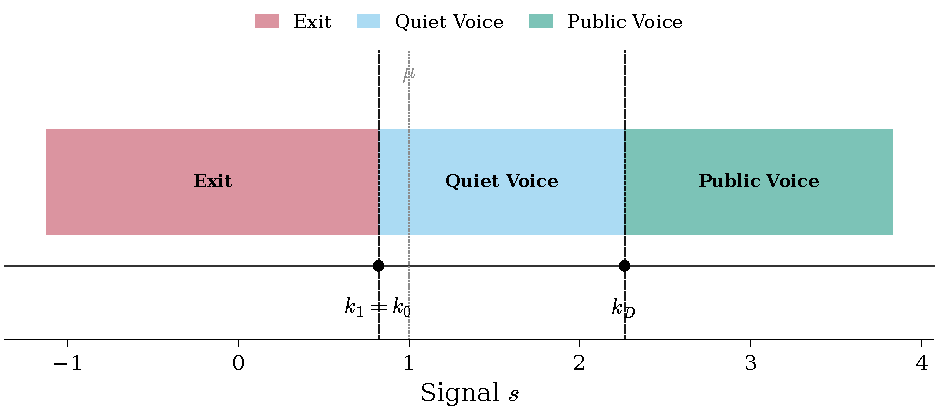
\includegraphics[width=0.9\textwidth]{numerical_output/fig_cutoff_structure.pdf}
\caption{Equilibrium cutoff structure. The blockholder follows a threshold strategy with weakly ordered cutoffs. In general, the signal space can be partitioned into up to four regions (Exit, Hold, Quiet Voice, Public Voice), with disclosure occurring only under Public Voice. In the baseline numerical example, $k_0=k_1$, so the strategy reduces to Exit, Quiet Voice, and Public Voice.}
\label{fig:cutoff-structure}
\end{figure}

\begin{figure}[H]
\centering
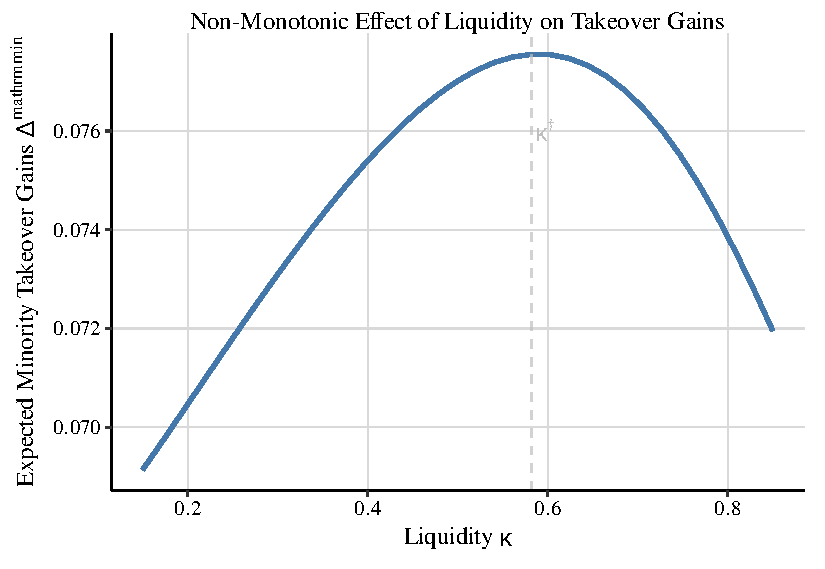
\includegraphics[width=0.85\textwidth]{numerical_output/fig_nonmonotone.pdf}
\caption{Nonmonotonic effect of liquidity on expected minority takeover gains. The vertical dashed line marks the turning point $\kappa^{\dagger}$ (the maximizer of $\Delta^{\min}$ on the plotted grid) in the baseline calibration.}
\label{fig:nonmonotone}
\end{figure}

\begin{figure}[H]
\centering
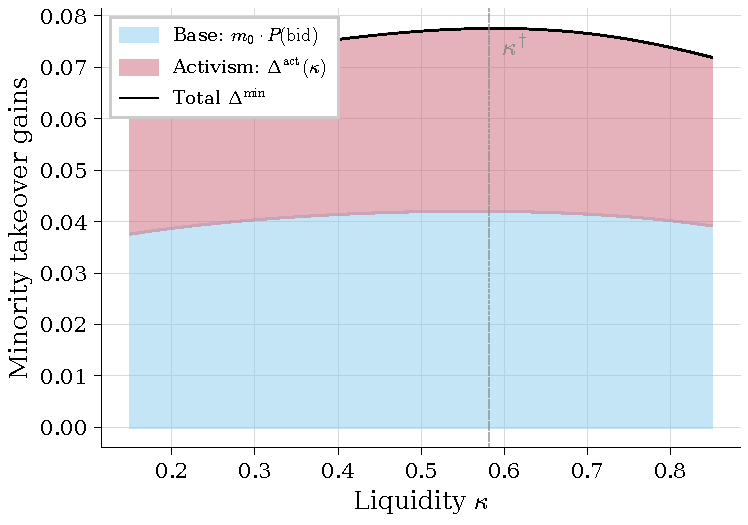
\includegraphics[width=0.85\textwidth]{numerical_output/fig_decomposition.pdf}
\caption{Decomposition of minority takeover gains. The base component $m_0 \cdot \PP(\textup{bid})$ and the activism component $\Delta^{\textup{act}}(\kappa)$ vary smoothly with liquidity in the baseline calibration; the dashed line marks $\kappa^{\dagger}$.}
\label{fig:decomposition}
\end{figure}

\begin{figure}[H]
\centering
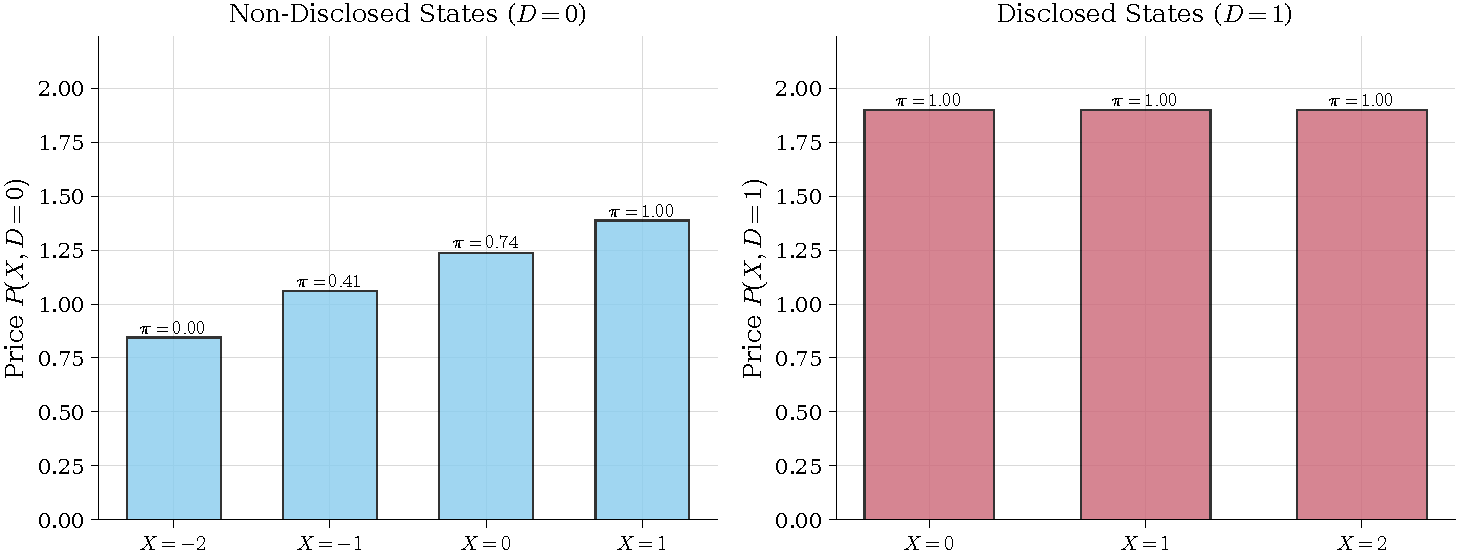
\includegraphics[width=0.95\textwidth]{numerical_output/fig_prices.pdf}
\caption{Equilibrium prices by state $(X,D)$ in the baseline numerical example. Left panel: nondisclosed states ($D=0$). Right panel: disclosed states ($D=1$). Bars are shown for on-path states under the calibrated strategy. Numbers above bars indicate the posterior engagement probability $\pi(X,D)$.}
\label{fig:prices}
\end{figure}

\begin{figure}[H]
\centering
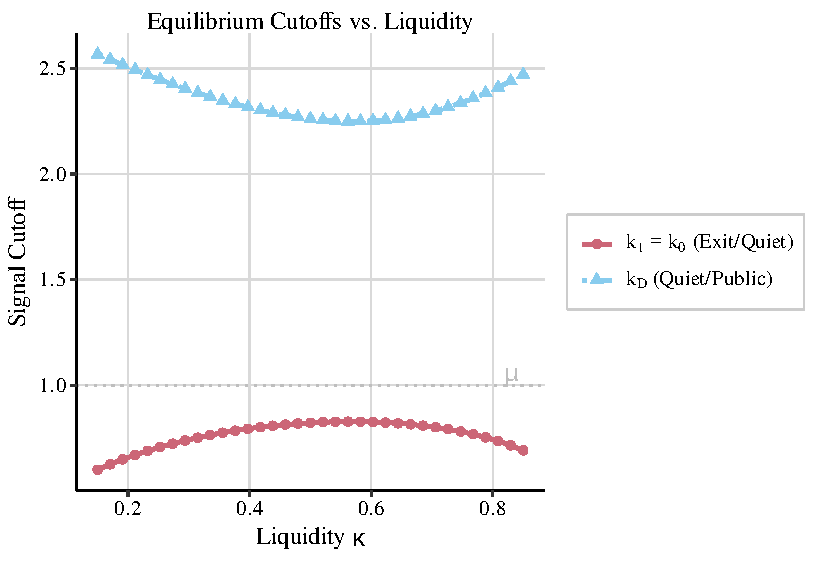
\includegraphics[width=0.85\textwidth]{numerical_output/fig_cutoffs_kappa.pdf}
\caption{Equilibrium cutoffs as functions of liquidity. The ordering $k_1 \le k_0 \le k_D$ is preserved; regions may collapse. The horizontal dashed line marks the prior mean $\mu$.}
\label{fig:cutoffs-kappa}
\end{figure}

\begin{figure}[H]
\centering
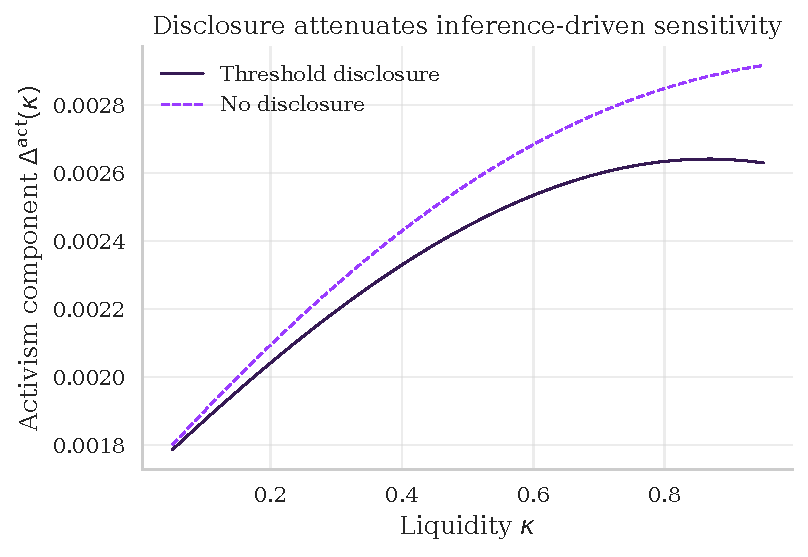
\includegraphics[width=0.85\textwidth]{numerical_output/fig_disclosure.pdf}
\caption{Disclosure attenuation through the inference channel (partial equilibrium in $\kappa$). We fix the blockholder's cutoff strategy at the baseline calibrated equilibrium ($\kappa=0.5$) and vary liquidity $\kappa$ only through the order-flow noise distribution. The blue curve plots $\Delta^{\textup{act}}(\kappa)$ under threshold disclosure with fixed cutoffs. The orange curve plots the counterfactual ``no-disclosure'' benchmark with the same fixed cutoffs, in which the market conditions only on order flow $X$.}
\label{fig:disclosure}
\end{figure}

\begin{figure}[H]
\centering
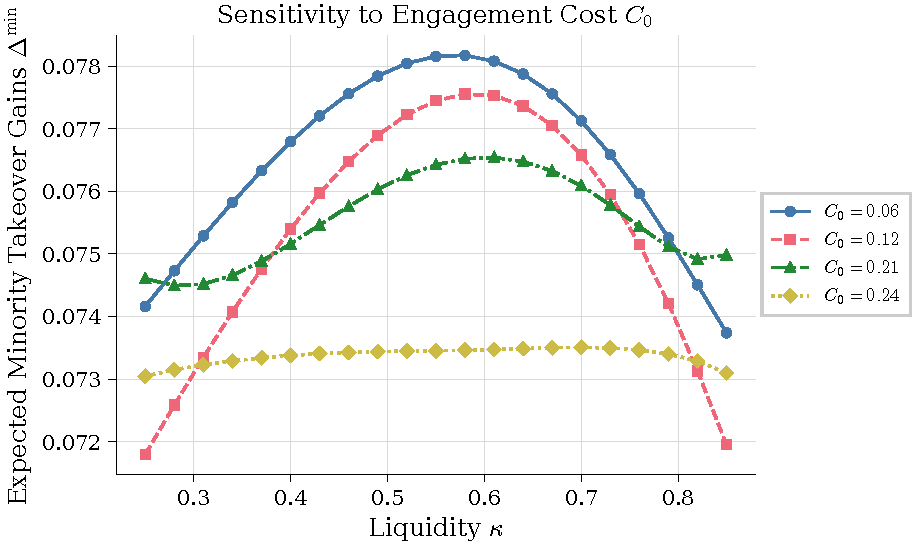
\includegraphics[width=0.85\textwidth]{numerical_output/fig_sensitivity_C0.pdf}
\caption{Sensitivity to engagement cost $C_0$. Expected minority takeover gains remain broadly nonmonotone in $\kappa$ across cost levels (computed over $\kappa \in [0.25,0.85]$), with the hump flattening at high $C_0$ as voice becomes rare. Higher costs shrink the voice regions and reduce the activism component, but can increase bid incidence; the net effect on $\Delta^{\min}$ is therefore ambiguous in general.}
\label{fig:sensitivity-C0}
\end{figure}

\begin{figure}[H]
\centering
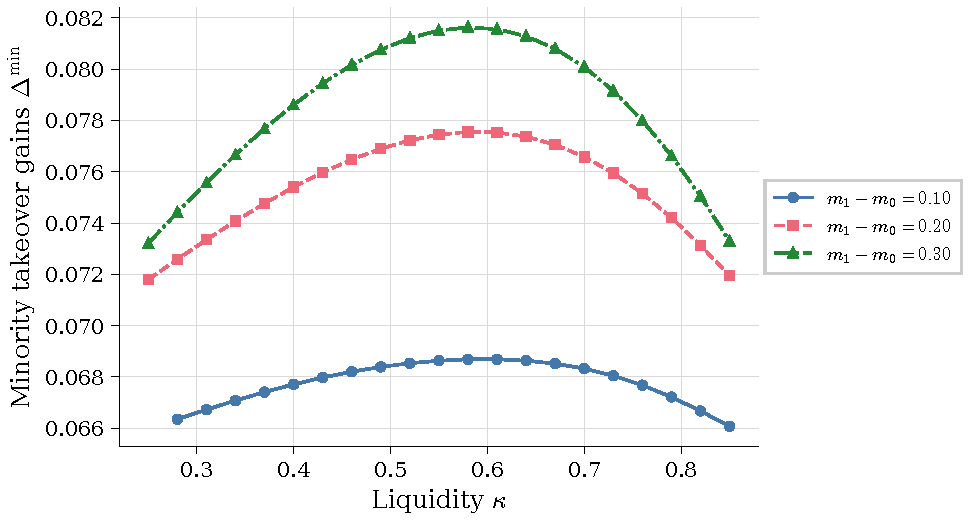
\includegraphics[width=0.85\textwidth]{numerical_output/fig_sensitivity_wedge.pdf}
\caption{Sensitivity to premium wedge $(m_1 - m_0)$. A larger wedge raises the premium conditional on bidding but can deter bids; expected minority takeover gains can therefore be nonmonotone in the wedge (computed over $\kappa \in [0.25,0.85]$).}
\label{fig:sensitivity-wedge}
\end{figure}

\begin{figure}[H]
\centering
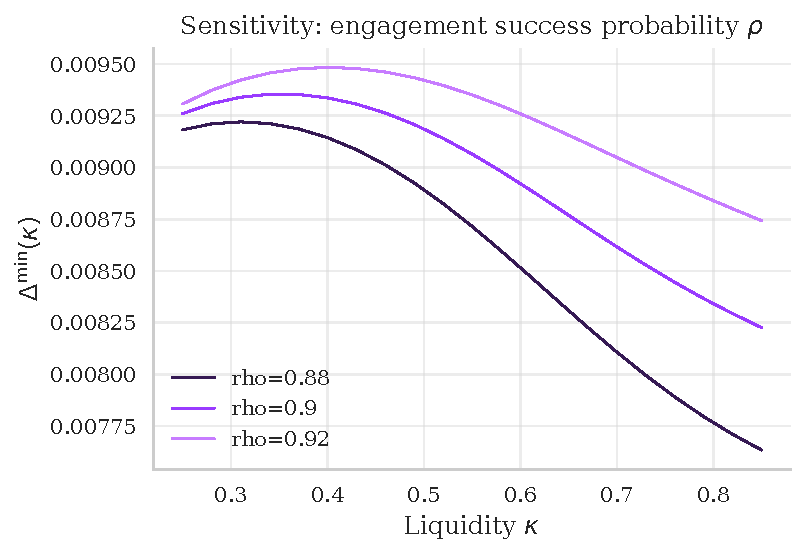
\includegraphics[width=0.85\textwidth]{numerical_output/fig_sensitivity_rho.pdf}
\caption{Sensitivity to engagement success probability $\rho$. Lowering the expected success rate naturally shrinks the magnitude of minority takeover gains, flattening the curve. However, the qualitative nonmonotonicity remains robust, driven by the structural trade-off between bid incidence and order-flow inference.}
\label{fig:sensitivity-rho}
\end{figure}

\begin{figure}[H]
\centering
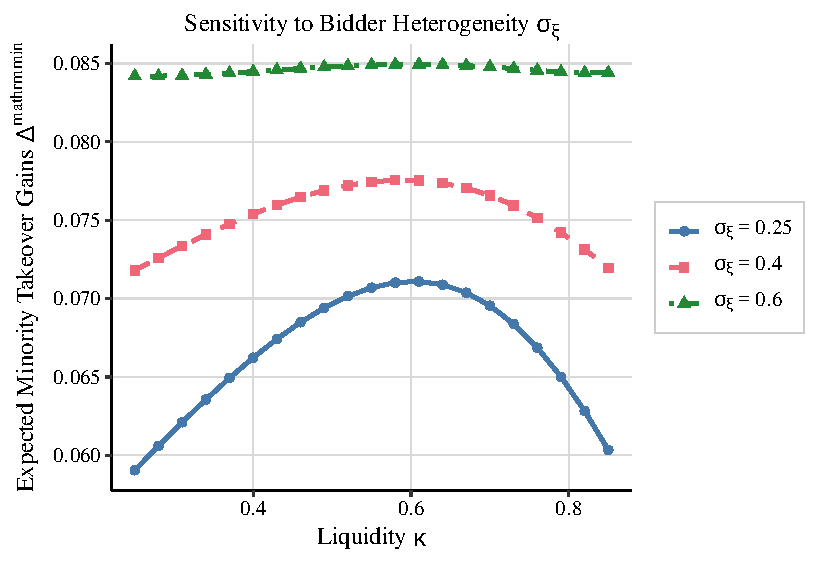
\includegraphics[width=0.85\textwidth]{numerical_output/fig_sensitivity_sigma_xi.pdf}
\caption{Sensitivity to bidder synergy volatility $\sigma_\xi$. Increasing bidder heterogeneity raises overall bid incidence, which uniformly shifts expected minority gains upward while preserving the inference-driven hump shape. Larger values of $\sigma_\xi$ also strictly relax the condition governing the price-to-entry feedback loop.}
\label{fig:sensitivity-sigma-xi}
\end{figure}

\begin{figure}[H]
\centering
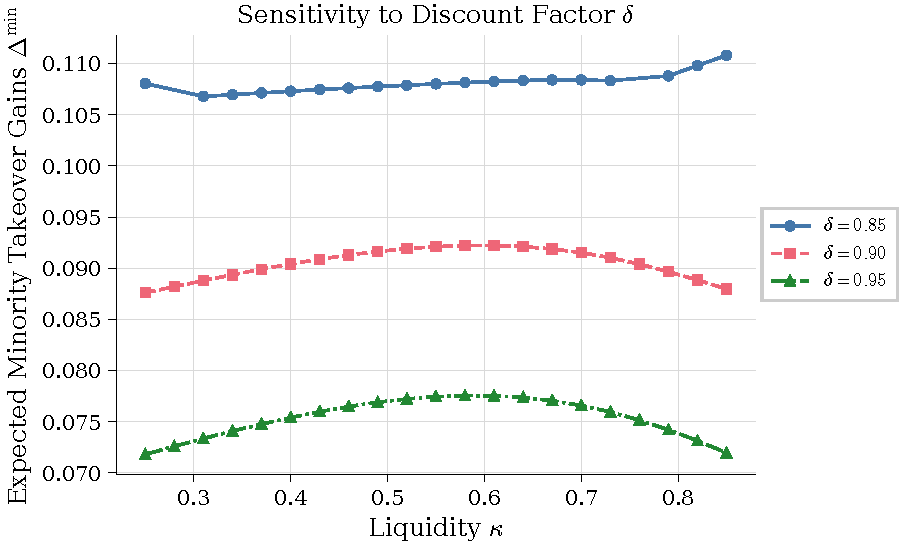
\includegraphics[width=0.85\textwidth]{numerical_output/fig_sensitivity_delta.pdf}
\caption{Sensitivity to the discount factor $\delta$. Lower discount factors mechanically reduce equilibrium prices, increasing bid incidence as the bidder faces lower acquisition costs. Although lower $\delta$ weakens engagement incentives, the bid-probability channel dominates, producing a uniform upward shift in minority gains and a progressive flattening of the hump shape.}
\label{fig:sensitivity-delta}
\end{figure}

\begin{figure}[H]
\centering
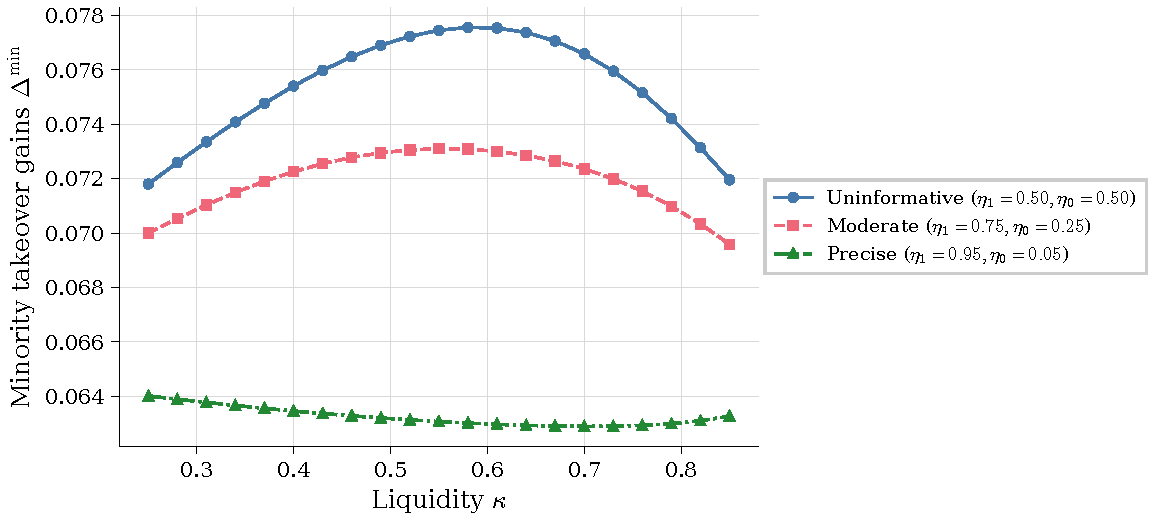
\includegraphics[width=0.85\textwidth]{numerical_output/fig_noisy_rumor_precision.pdf}
\caption{Disclosure attenuation via noisy rumors. Under the intermediate information regime, the market receives an imperfect signal of hidden engagement. As the public rumor becomes more precise ($\eta_1 - \eta_0$ increases), engagement becomes more observable in nondisclosed states, progressively flattening the sensitivity of the activism premium to market liquidity.}
\label{fig:noisy-rumor-precision}
\end{figure}

\begin{figure}[H]
\centering
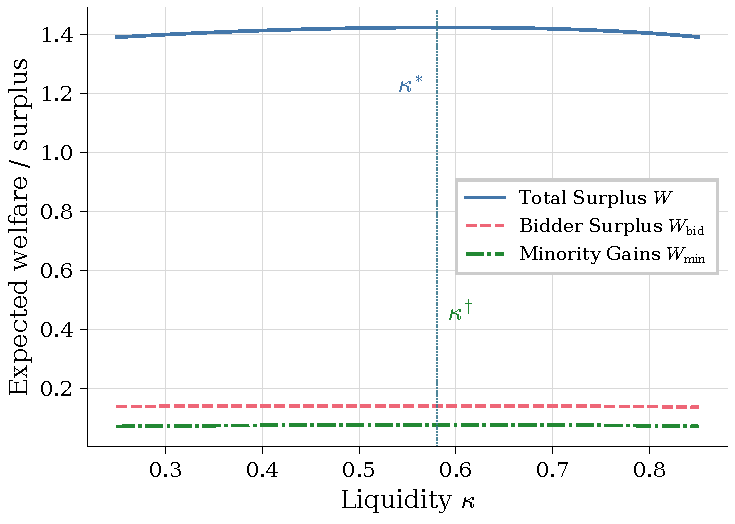
\includegraphics[width=0.85\textwidth]{numerical_output/fig_welfare.pdf}
\caption{\textbf{Welfare and the liquidity hump.} Expected total surplus $W$
and its components---blockholder payoff $W_B$, minority gains $\Delta^{\min}$,
and bidder surplus $W_{\textup{bid}}$---against noise-trading intensity
$\kappa$. By Lemma~\ref{lem:endpoints} minority value creation is
endpoint-symmetric, $\Delta^{\min}(0)=\Delta^{\min}(1)>0$: it does \emph{not}
vanish at the extremes. The interior hump is \emph{conditional}---it obtains
under condition~(W$^{\ast}$) and inverts to a trough when the condition
fails---and the total $W$ peaks at $\kappa^{\ast}$, which may differ from the
minority optimum $\kappa^{\dagger}$ (the planner's wedge of
Proposition~\ref{prop:planner-wedge}). At the baseline calibration the two
optima nearly coincide.}
\label{fig:welfare}
\end{figure}

\end{document}
